	\documentclass[12pt, a4paper]{report}
\usepackage[utf8]{inputenc}
	\usepackage[norsk, english]{babel}
\usepackage[toc,page]{appendix}
\usepackage{cite}
\usepackage{hyperref}
\usepackage{color}
\usepackage{rotating}
\usepackage{adjustbox}
\usepackage{caption}
\usepackage{xcolor}
\usepackage{afterpage}
\usepackage{multirow}
\usepackage{enumitem}
\usepackage[colorinlistoftodos]{todonotes}
%%===================================
%Write the various parts of your thesis as separate files and include them into the main file by the command \include{name of included file}. When you compile the LaTeX file, you may choose which subfiles to include by the command

%\includeonly{chapter01,chapter02}

%%===================================
\begin{document}
\listoftodos
\pagenumbering{roman}
\begin{abstract}

Agile retrospectives could help team learn from the past and identify improvement opportunities. In this thesis we investigate the characteristics of the present retrospective practice and the organizational learning it provides for teams practicing them, through a multiple case-study. 

The research is based on a depth-study of five years of retrospective practice from one team, and a breadth-study of seven interviews from other retrospective practicing teams. 

Our results shows that teams today is mostly satisfied with their retrospective practice and are able to identify improvement opportunities and implement them, which contradicts previous research\cite{Drury2012}. However we identify one barrier related to team commitment dependent on enthusiasm and previous implementation of improvement opportunities that results in a feedback-loop that could both help implement future improvements and hinder it. We investigate the learning happening through todays retrospectives and finds that the practice is approximating an Organization Learning II system \cite{Argyris1996}, with most of the governing values and behavioral consequences is present in todays practice. However we find that the primary learning type remains single-loop even though double-loop should be expected. We identify a barrier that hinders double-loop learning consisting of several factors and propose a method based on our findings that can lower this barrier. 

Finally we conclude that todays retrospective practices provide agile development teams to adapt their current work-practices and enables them to learn from past development iterations and thus provide the means for identifying improvements opportunities and improve from them.

\end{abstract}
\setcounter{page}{1}
\clearpage
\setcounter{page}{2}
\setcounter{tocdepth}{3}
\tableofcontents
\listoffigures
\listoftables
\clearpage
\setcounter{page}{0}
\pagenumbering{arabic}
\chapter{Introduction}
\todo{Write Introduction}
\section{Background}
\todo[inline]{Write background}
\section{Research Objective}
\todo[inline]{Write Research Objective}
\section{Agile Development}
\todo[inline]{Theory on Agile Development}

\section{Retrospective}
Retrospectives, sometimes also called postmortems, is a activity that aim to improve learning within an organization. We will look at different retrospective definitions, some common techniques used and some of the earlier academic work in the following subsection. 

\subsection{Retrospective Definition}
There are several different definitions of retrospectives. Dingsøyr \cite{Dingsoyr2004} defines postmortem as: 

\begin{quote}
By a postmortem, we mean a collective learning activity which
can be organised for projects either when they end a phase or
are terminated. The main motivation is to reflect on what happened
in the project in order to improve future practise—for the
individuals that have participated in the project and for the organisation
as a whole. The physical outcome of a meeting is a
postmortem report.
\end{quote}

\todo[inline]{Add a retrospective definition of diana larsen mayhaps?, if not found use tiedeman.}

We have created another definition on the retrospective as Dingsøyr's definition limit the retrospective to the end of a project or a phase of the project. 

\begin{quote}
	\textit{Retrospectives is a process that aims to facilitate shared learning within a team or an organization after a learning event, and such create a focus that aims to improve the current work practices.}
\end{quote}

We say learning event as different teams holds retrospectives after different kinds of events. We list the kinds of retrospectives known to us in \autoref{table:retrospective-types}. For this paper our main focus will be related to what we call iteration retrospectives, which is the practice commonly used in SCRUM and Kanban. 

\begin{table}[h]
	\begin{center}
		\caption{Types of retrospectives}
		\label{table:retrospective-types}
		\begin{tabular}{l l}
			\hline
			Retrospective Type & Description \\
			\hline
			Iteration Retrospective & Held after project iteration \\
			Project Retrospective & Held after a project ends \\
			Feature Retrospective & Held after the release of a feature \\
			Incidents Retrospective & Held after an incident \\
			Back-on-track retrospective & Held when work practices is failing \\
			\hline
		\end{tabular}
	\end{center}
\end{table}

\subsection{Retrospectives Techniques}
There are a lot of ways to perform retrospective. Around the table discussion, story-telling, weather-forecast and many more are examples of ways to conduct retrospectives. We will briefly describe two commonly used technique called KJ-session and timeline. Other techniques can be found by reading Derby and Larsen's book\cite{Larsen2006}: \textit{``Agile Retrospectives: Making Good Teams Great!''}, accessing the web page Retromat.org\cite{retromat2015} or reading our own literature review on the agile retrospective\cite{Dolvik2014}. 

\subsubsection{KJ-session}
KJ-sessions are a commonly used brainstorming technique where each participant write issues on post-it notes after the participants are done the post-it notes are grouped and discussed in the group. Dingsøyr, Moe and Nytrø\cite{Moe2001} provides an example of they conducted a KJ-session and the end-result of a KJ-session can be seen in \autoref{figure:kj-session}: 

\begin{quote}
We used a technique named after a Japanese ethnologist, Jiro
Kawakita - called the KJ-method. For each of these sessions,
we give the participants a set of post-it notes, and ask them to
write one issue on each. We usually hand out between three and
five notes per person, depending on the number of participants.
After some minutes, we ask one of them to attach one note to a
whiteboard and say why this issue was important. Then the next
person would present a note and so on until all the notes are on
the whiteboard. The notes are then grouped, and each group is
given a new name. 
\end{quote}

\begin{figure}[!h]
	\centering
	
\includegraphics[width=\textwidth, keepaspectratio]{figures/KJ-session.png}
	\caption{KJ-session end result, provided by Dingsøyr\cite{Dingsoyr2004}}
	\label{figure:kj-session}
\end{figure}

\subsubsection{Timeline}
Timeline is an activity that lets the participants create a timeline over the last learning event and reflect on the event during the creation. Derby and Larsen\cite{Larsen2006} suggests that the participants should be divided into multiple groups. Each member in the group should then be handed markers and post-it notes and then write their own issues from the learning event down. Derby and Larsen suggests color-coding the post-it notes relating them to feelings, events, functions or themes. When all the participants are done writing they should together create a timeline with the post-it notes. After the timeline is done the group should analyze the timeline, looking for interesting patterns and opportunities for future improvements. An example timeline is shown in \autoref{figure:timeline}.

\begin{figure}[!h]
	\centering
	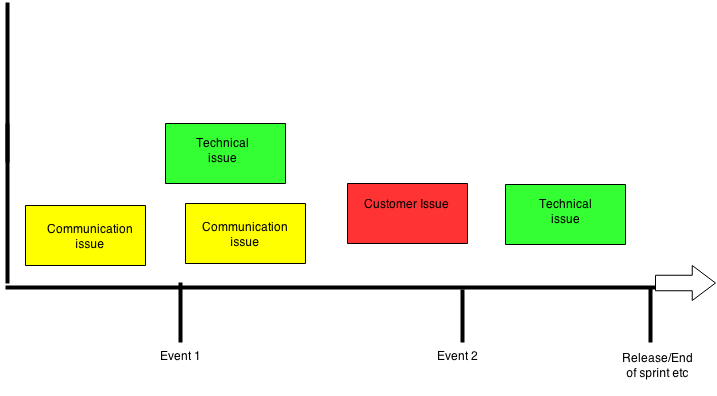
\includegraphics[width=\textwidth, keepaspectratio]{figures/Timeline-Example.png}
	\caption{Timeline illustration}
	\label{figure:timeline}
\end{figure}

There also exists a variation of timeline called; Evidence-Based Timelines, which is described by Bjarnason and Regnell\cite{Bjarnason2012}. The difference from normal timeline retropsective is that the data is collected through available systems before the retrospective. The idea is to counter bias from the participants where memory lacks and thus rather use data collected from available system during the time-period in question. A graphic example is presented by Bjarnason and Regnell and shown in \autoref{figure:e-b-timeline}. 

\begin{figure}[!h]
	\centering
	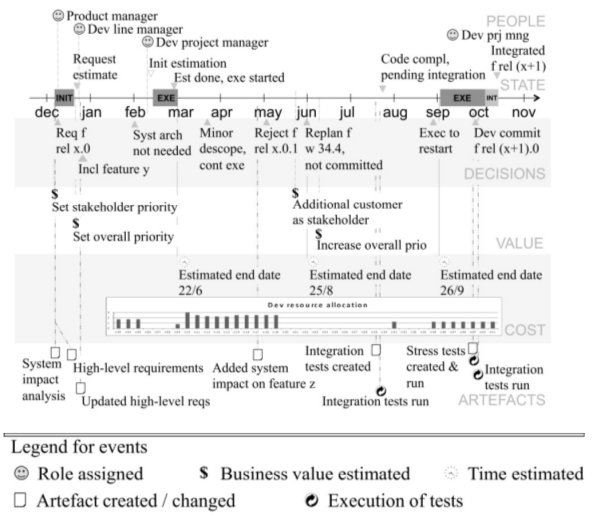
\includegraphics[width=\textwidth, keepaspectratio]{figures/eb-timeline.png}
	\caption{Evidence-based timeline illustration, presented by Bjarnason and Regnell\cite{Bjarnason2012}}
	\label{figure:e-b-timeline}
\end{figure}

\subsection{Retrospectives: Earlier Academic Work}
There have been several articles, conference papers, and experience reports on retrospectives or mentioning them as part of agile development.

Dingsøyr, Moe and Nytrø compared light-weight postmortem review against experience reports and found that the two provides different kind of experience. light-weight postmortem focuses on implmentation, administration, developers and maintence, while experience reports yield experience related to contract issues, design and technology. 

On the subject of retrospectives techniques several publications has been done. Stålhane, Dingsøyr, Hanssen and Moe\cite{Hanssen2003} compared two methods of semi-structured interviews and KJ-session and found that both may be applied to harvest knowledge. Bjarnason and Regnell\cite{Bjarnason2012} proposed the evidence-based timelines method as a way of conducting retrospectives. Bjørnson, Wang and Arisholm\cite{bjornson2009} compared the effectiveness of root-cause analysis against that of fishbone diagrams and found that root-cause analysis was more effective as the fishbone diagram limits the way issue were related to each other. Dingsøyr\cite{Dingsoyr2004} have written an article on the subject highlighting the purpose of the retrospective as well as discussing three possible approaches. Dølvik and Stålesen\cite{Dolvik2014} did a literature review on agile retrospectives and found that different techniques would fit different goals, and they found a lack of research considering follow-up on the issues identified during the retrospective. There also several experience reports on the subject, two of them Maham\cite{Maham2008}, Kinoshita\cite{Kinoshita2008}, which describes how to plan and facilitate retrospectives as well as describing different techniques. Finally Derby and Larsen\cite{Larsen2006} has as previously mentioned a book on the subject. 

Other work returns some different findings. Drury, Conboy and Power\cite{Drury2012} in a study on obstacles to decision making in agile development team that SCRUM-master prioritizes other tasks than follow-up on actions from retrospectives. They proposed that discussion on decision-making should be a part of the retrospective. And they found that some regarded the retrospective as a waste of time while others found it useful. Comparing to this Stålhane, Dingsøyr, Hanssen and Moe\cite{Hanssen2003} found that the participants of their case-study regarded the postmortem as useful. 

Zedtwitz\cite{Zedtwitz2002} identified several barriers for learning in post-project reviews in R\&D. Two psychological barriers were identified; inability to reflect and memory bias. Managerial barriers were time constraints and bureaucratic overhead. Epistemological barriers such as difficult to generalize and tacitness of process knowledge were also identified by Zedtwitz. The last barriers were team-based and identified as reluctance to blame and poor internal communication. 

There are several publications mentioning retrospectives or directly address them, however most of these studies are related to how one should conduct retrospectives or the purpose of it. However we have not seen any studies addressing the value of the retrospective, which is in part why we have focused to conduct this case study. 
\clearpage

\section{Organizational Learning}
\label{intro:organizational-learning}
Organizational learning is in simple terms how an organization is able to acquire, store and utilize knowledge existing within an organization. In a more academic setting we can use Argyris and Schön definition \cite{Argyris1996} for organizational learning: 

\begin{quote}
	``Organizational learning occurs when individuals within an organization experience a problematic situation and inquire into it on the organization's behalf. They experience a surprising mismatch between expected and actual results of action and respond to that mismatch through a process of thought and further action that leads them to modify their images of organization or their understandings of organizational phenomena and to restructure their activities so as to bring outcomes and expectation into line, thereby changing organizational theory-in-use. In order to become organizational, the learning that results from organizational inquiry must become embedded in the images of organization held in its members' minds and/or in the epistemological artifacts (the maps, memories, and programs) embedded in the organizational environment. ''
\end{quote}

Organizational learning can be applied to groups of people over different sizes. One can use it to analyze huge organizations consisting of many actors in different roles, or small groups of people working close together. For this research we are going to apply the organizational learning at an agile development team. 

Different types of frameworks exist for organizational learning. Levitt and March uses a framework that see learning in organizations as encoding inferences from history into routines that guide behavior \cite{Levitt1988}. The retrospective is a process of shared learning for an agile development team learning from the last iteration of development. Investigating learning using this framework won't yield much as the retrospective already is seen as a collective learning activity \cite{Dingsoyr2004}. 

Argyris and Schön \cite{Argyris1996} uses two different models to determine how an organization learns through individuals, Model I and Model II. As agile teams often are limited to a close group of individuals we will apply Argyris and Schön's models. To understand these models we first need to investigate two types of learning: Single-loop learning and double-loop learning. Further in this section we will explain these types of learning as well as Model I and Model II. We have borrowed \autoref{table:model-I}, \autoref{table:model-II}, \autoref{table:social-virtues} from Argyris and Schön's ``Organizational learning II: Theory, Method and Practice''\cite{Argyris1996} and they provide a quick overview of the two models as well as the social virtues that differs between them. We will also look at Triple-loop learning as it is the concept of learning about learning. 

\subsection{Single-loop}
Single-loop learning is a type of learning defined by Argyris and Schön. It consist of a single-feedback loop that finds an error and a way to fix this problem. Argyris and Schön \cite{Argyris1996} defines single-loop as: 

\begin{quote}
``By single-loop learning we mean instrumental learning that changes strategies of action or assumptions underlying strategies in ways that leave the value of a theory of action unchanged.

... In such learning episodes, a single feed-back loop, mediated by organizational inquiry, connects detected error - that is, an outcome of action mismatched to expectations and, therefore, surprising - to organizational strategies of action and their underlying assumptions. These strategies of action and their underlying assumptions. These strategies or assumptions are modified, in turn, to keep organizational performance within the range set by existing organizational value and norms. The values and norms themselves ... remain unchanged. 
''
\end{quote}

An example of single-loop learning from software development could be finding a bug, find a solution to fix it and the fix it. The single-loop learning would here be learning the solution and fixing the bug. We have provided a basic illustration of single-loop learning in \autoref{figure:single-loop}.

\begin{figure}[!h]
	\centering
	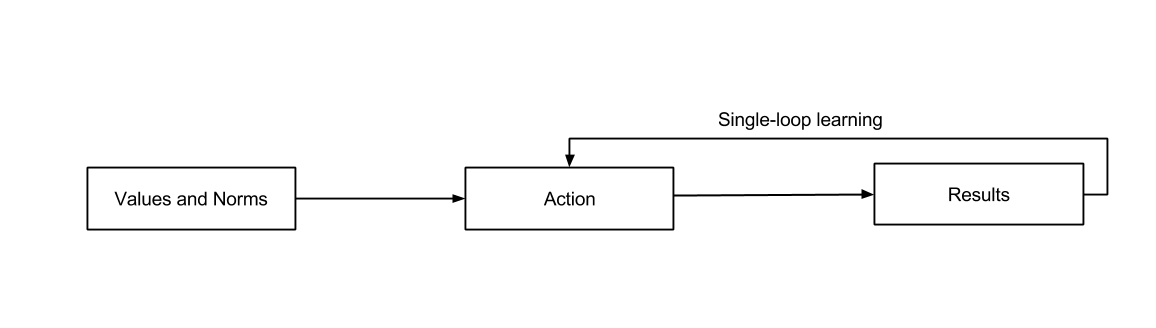
\includegraphics[width=\textwidth, keepaspectratio]{figures/Single-loop.png}
	\caption{Single-loop learning.}
	\label{figure:single-loop}
\end{figure}

\subsection{Double-loop} % (fold)
\label{sub:double_loop}
Double-loop learning is a type of learning where one ask whether the underlying factors that influence the actions and results is sufficient.
One might say that one understand the root-cause for the issue. 
Argyris and Schön defines double-loop learning as: 

\begin{quote}
``By double-loop learning, we mean learning that results in a change in the values of theory-in-use, as well as in its strategies and assumptions. The double loop refers to the two feedback loop that connect the observed effects of actions with startegies and values server by strategies. Strategies and assumptions may change concurrently with, or as a consequence of, change in values. Double-loop learning may be carried out by individuals, when their inquiry leads to change in the values of their theories-in-use or by organizations, when indivduals inquire on behalf of an organization in such a way as to lead to change in the values of organization theory-in-use. ''
\end{quote}

This type of learning can be shown in our bug example. If the developers who earlier found and fixed a bug did a root-cause analysis on the issue they could get several results indicating that underlying factors are not sufficient for the current state of development team. One underlying factor could be weak specification description requiring the team to rethink and restructure how they develop specifications. Another reason could be that the knowledge for the system are not good enough with the developers indicating a knowledge-gap in the team and considerations for the state of the team may be required. 

For this research we use the term double-loop learning when the influences for the issue is understood and change occurs as a results of this. A simple figure of double-loop learning can be seen in \autoref{figure:double-loop}

\begin{figure}[!h]
	\centering
	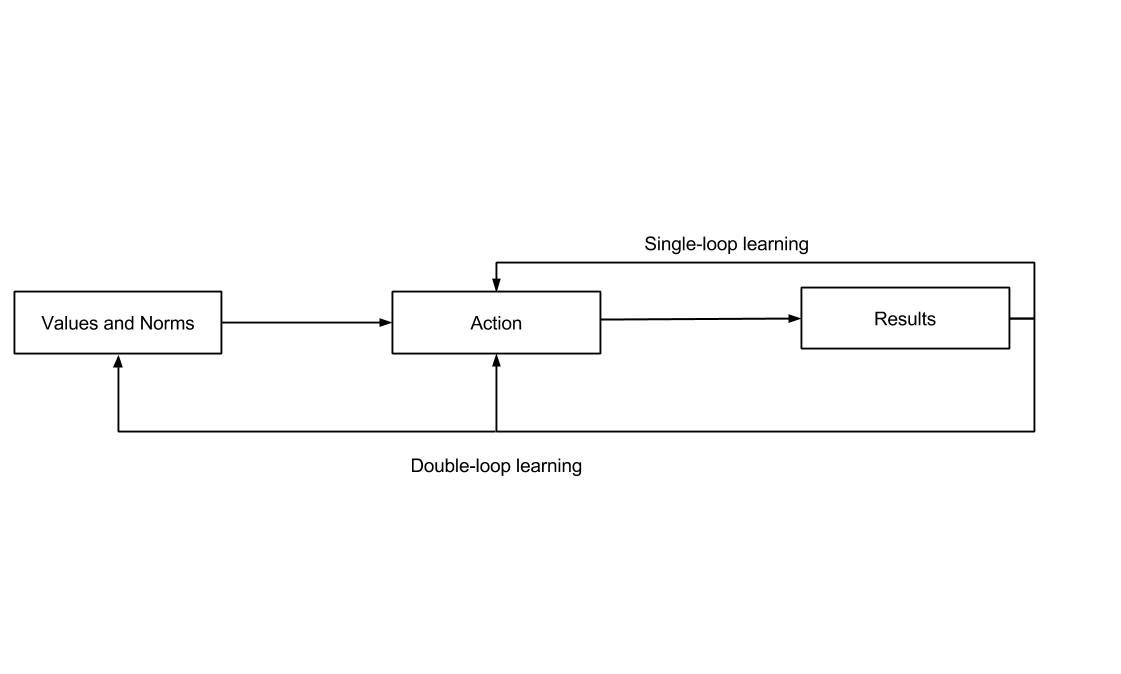
\includegraphics[width=\textwidth, keepaspectratio]{figures/double-loop.png}
	\caption{Double-loop learning.}
	\label{figure:double-loop}
\end{figure}

% subsection triple_loop (end)
\subsection{Model I} % (fold)
\label{sub:model_i}
Argyris and Schön \cite{Argyris1996} describes a learning system called Organizational learning I, which theory-in-use is described as Model I. As organizational learning I is employed learning system that can be defined by different actions and implementations we will instead go into the theory-in-use, Model I, as these systems employ them.

Argyris and Schön \cite{Argyris1996} describes Model I through its governing variables. We will go through each of them along with the actions strategies, consequences for behavioral world and consequences for learning, effectiveness that follows of the different governing variables that actors try to satisfy. 

The first governing value described is defining goals and try to achieve them. This leads to the action strategies of designing and manage the environment unilaterally. The behavioral consequences are that the actor gets seen as defensive, inconsistent, incongruent, controlling, fearful of being vulnerable, withholding feelings, overly concerned about self and others, or under-concerned about others. For the effectiveness and learning the consequences are that the actor are self-sealing and the longterm effectiveness is decreased. 

Maximize winning and minimize losing is the second governing variable that the actors in an organization try to satisfy. The actions strategies for this governing value is that the actor takes ownership and control of a task. This results in a defensive interpersonal and group relationship where the actor wants the rest of the group to see things his way and little help could be a result of this. For terms of learning this will provide single-loop learning as the output of the task his more important than the task itself. 

The third governing value for the actors in this kind of learning model is minimizing generating or expressing negative feelings. The action strategy that follows is that the actors wishes to protect themselves using defensive actions such as blaming, stereotyping and suppressing feelings. The consequences for the behavioral world is defensive norms within the organizations. Rivalry, lack of external commitment and mistrust are examples of such norms. For the learning consequences of this value little theories will be tested publicly prohibiting double-loop learning in the organization. However there will still be much testing of theories with the individuals however this knowledge will not reach the organization. 

Being rational is the fourth and final governing variable for Argyris and Schön's Model I theory-in-use for the learning organization. Being rational provides the action strategy of protecting other from being hurt resulting in actions like withholding information, creating censoring rules that can censor information and behavior. This returns the same consequences for the behavioral world, learning and effectiveness as described above. 

Through the governing values of Model I the actors within the organization prohibits double-loop learning. The organization creates a win or loose situation between the actors leading to withholding of information, mistrust between the actors and little testing of current norms of values. This again provides competition instead of collaboration and thus have a negative impact on the learning and effectiveness of the organization. Model I is further described by Argyris and Schön as the different elements of the model interact in complex ways. This can be read about in ``Organizational learning II: Theory, Method and Practice'' \cite{Argyris1996}.

\begin{sidewaystable}[!h]
	\begin{center}
	\caption{Theory-in-use of Organizational learning I borrowed from ``Organizational learning II: Theory, Met hod and Practice'' by Argyris and Schön \cite{Argyris1996}}
	\label{table:model-I}
	\makebox[\textwidth]{%
		\begin{tabular}{ p{0.25\textwidth} p{0.25\textwidth} p{0.25\textwidth} p{0.25\textwidth} }
		\multicolumn{4}{l}{\textit{Model I Theory-in-Use}} \\
		\hline
		\textbf{Governing Variables} & \textbf{Action Strategies} & \textbf{Consequences for Behavioral World} & Consequences for Learning, Effectiveness \\
		Define goals and try to achieve them. & Design and manage the environment unilaterally (be persuasive, appeal to larger goals, etc.) & Actor seen as defensive, inconsistent, incongruent, controlling, fearful of being vulnerable, withholding of feelings, overly concerned about self and others, or under-concerned about others. & Self-sealing. 

		Decreased Long-term effectiveness. \\
		Maximize winning and minimize loosing. & Own and control the task (claim ownership of the task, be guardian of the definition and execution of the task). & Defensive interpersonal and group relationship (depending on actor, little help to others). & Single-loop learning. \\
		Minimize generating or expressing negative feelings. & Unilaterally protect yourself (speak in inferred categories accompanied by little or no directly observable data, be blind to impact on others and to incongruity; use defensive actions such as blaming, stereotyping, suppressing feelings, intellectualizing). & Defensive norms (mistrust, lack of risk taking, conformity, external commitment, emphasis on diplomacy, power-centered competition and rivalry). & Little testing of theories publicly. 

		Much testing of theories privately. \\
		Be rational. & Unilaterally protect others from being hurt (withhold information, create rules to censor information and behavior, hold private meetings). & & \\
		\hline
		\end{tabular}
	}
	\end{center}
\end{sidewaystable}

% subsection model_i (end)
\subsection{Model II} % (fold)
\label{sub:organizational_learning_ii}
The second model described by Argyris and Schön is the theory-in-use for organizational learning II systems called Model II. While Model I is creating a win-loose relationship between the actors resulting in actors trying to control the environment, Model II instead invites the actors to confronts each others views and emotions. This is creating an environment for double-loop learning where the actors strive to get the most complete understanding of their environment and adapt this. 

There are three governing values for Model II according to Argyris and Schön: Valid information, Free and informed choice and Internal commitment to the choice and constant monitoring of its implementation. 

The three governing values gives primarily four behavioral strategies. ``Designing situations where participants can be origins of action and experience high personal causation'' is one the strategies according Argyris and Schön. Another of these strategies is that the group of actors jointly control the tasks. This provides an environment where face-saving for the individual should not be needed and thus facilitates open and clear communication between the different actors. This again is connected to the third action strategy that is ``Protection of self is a joint enterprise and oriented towards growth''. The three governing values also provides an environment of bilateral protection towards others. 

There are several consequences for the behavioral world following the governing values and behavioral strategies for Model II. The first one is that actors within the organization acts less defensively than in Model I system and is experienced as minimally defensive. The second consequence is the same as the first one except that it relates to the relationship between the different individuals in the organization. The group dynamics and interpersonal relationships will be minimally defensive. As an organization approaches the practices that supports the three governing values learning-oriented norms will start appearing the in organization as a consequence. The final consequence Argyris and Schön describes is high freedom of choice, internal commitment and risk taking within the organization. 

As for the consequences on learning Model II will support double-loop learning. Disconfirmable processes and frequent public testing of theories will both support double-loop learning. As the defensive stance of the actors and relationships are minimized Model II practices will advocate and allow the organization to test their current theories on how their organization is performing, allowing for double-loop learning. 

As described by Argyris and Schön the Model II will in the long term increase effectiveness within an organization. Through facilitating collaboration rather than competition, allowing testing of the currently perceived world and norms and allowing experimentation the Model II allows double-loop learning. Being able to adapt the organization through double-loop learning will in the long term increase the effectiveness. 

Finally the Modell II theory-in-use is not a goal one can achieve as described by Argyris and Schön. Instead it is a focus one can work against, as the nature of the Modell II and double-loop learning is always to challenge the current world for better one can never achieve the ideal world as this world will always be able to change and improve. 

\begin{sidewaystable}[!h]
	\begin{center}
	\caption{Theory-in-use of Organizational learning II borrowed from ``Organizational learning II: Theory, Method and Practice'' by Argyris and Schön \cite{Argyris1996}}
	\label{table:model-II}
	\makebox[\textwidth]{%
		\begin{tabular}{p{0.2\textwidth} p{0.2\textwidth} p{0.2\textwidth} p{0.2\textwidth} p{0.2\textwidth}}
		\multicolumn{5}{l}{\textit{Model II Theory-In-Use}}\\
		\hline
		\textbf{Governing Variables for Action} & \textbf{Action Strategies} & \textbf{Consequences of Behavioral World} & \textbf{Consequences on Learning} & \textbf{Consequences on effectiveness} \\
		\hline
		\begin{itemize}[leftmargin=*]
			\item[] Valid information
			\item[] Free and informed choice 
			\item[] Internal commitment to the choice and constant monitoring of its implementation
		\end{itemize}
		&
		\begin{itemize}[leftmargin=*]
			\item[] Design situations where participants can be origins of action and experience high personal causation
			\item[] Task is jointly controlled
			\item[] Protection of self is a joint enterprise and oriented toward growth
			\item[] Bilateral protection of others
		\end{itemize}
		&
		\begin{itemize}[leftmargin=*]
			\item[] Actor experienced as minimally defensive
			\item[] Minimally defensive interpersonal relations and group dynamics
			\item[] Learning-oriented norms
			\item[] High freedom of choice, internal commitment, and risk taking 
		\end{itemize}
		& 
		\begin{itemize}[leftmargin=*]
			\item[] Disconfirmable processes
			\item[] Double-loop learning
			\item[] Frequent public testing of theories
		\end{itemize}
		& Increased long-term effectiveness \\
		\hline
		\end{tabular}
	}
	\end{center}
\end{sidewaystable}

\begin{table}[!h]
	\begin{center}
	\caption{Social Virtues of Model I and Model II borrowed from ``Organizational learning II: Theory, Method and Practice'' by Argyris and Schön \cite{Argyris1996}}
	\label{table:social-virtues}
	\makebox[\textwidth]{%
		\begin{tabular}{ p{0.5\textwidth}  p{0.5\textwidth} }
		\textit{Model I Social Virtues} & \textit{Model II Social Virtues} \\
		\hline
		\textbf{Help and Support} & \\
		Give approval and praise to others. Tell others what you believe will make them feel good about themselves. Reduce their feelings of hurt by telling them how much you care and, if possible, agree with them that the others acted improperly. & Increase the other's capacity to confront their own ideas, to create a window into their own mind, and to face the unsurfaced assumptions, biases, and fears that have informed their actions toward other people. \\ 
		\\
		\textbf{Respect for Others} & \\
		Defer to other people; do not confront their reasoning or actions. & Attribute to other people of high capacity for self-reflection and self-examination without becoming so upset that they lose their effectiveness and their sens of self-responsibility and choice. Keep testing this attribution. \\
		\\
		\textbf{Strength} & \\
		Advocate your position in order to win. Hold your own position in the face of advocacy. Feeling vulnerable is a sign of weakness. & Advocate your position and combine it with inquiry and self-reflection. Feeling vulnerable while encouraging inquiry is a sign of strength. \\
		\\
		\textbf{Honesty} & \\
		Tell other people no lies, or tell others all you think and feel. & Encourage yourself and other people to make public tests of their ability to say what they know yet fear to say. Minimize what would otherwise be subject to distortion and cover-up of the distortion. \\
		\\
		\textbf{Integrity} & \\
		Stick to your principles, values, and beliefs. & Advocate your principles, values, and beliefs in a way that invites inquiry into them and encourages other people to do the same. \\
		\hline
		\end{tabular}
	}
	\end{center}
\end{table}

% subsection organizational_learning_ii (end)
% subsection double_loop (end)
\subsection{Triple-loop} % (fold)
\label{sub:triplloop}
The term tripleloop learning has been used in different ways as highlighted by Tosey, Visser and Saunders \cite{Tosey2011}. Triple-loop learning can be referred to both triple-loop learning and deutoro-learning. For this work we are going to stick with triple-loop learning. Tosey, Visser and Saunders performed a critical review of the triple-loop learning concept and finds that three concepts have been widely used in academic literature. 

The first concept they investigate is a form for learning above double-loop learning that addresses some learning in a level above the governing variable of double-loop learning. Tosey et. al. finds that this concept seem to be poorly defined, imprecise and unfounded in the way it is used. 

The second concept describes triple-loop learning as a form for meta-learning, a form of learning not above single-loop and double-loop, but rather beside. Learning about learning is a simple description. Tosey et. al. Finds that this concept is a renaming of deutoro-learning and raises the question if this renaming is needed. 

The final concept connects triple-loop learning to Bateson's Learning III, which can be read about in ``Gregory Bateson on deutero-learning and double bind: A brief conceptual history'' by Visser \cite{Visser2003}. This concept relates to a type of learning that is non-instrumental and exists beyond language. Tosey et. al. finds that the literature that uses this concept have not been conducting a comprehensive working-through of Bateson's Theory. 

For our research we are going to use the second concept, where triple-loop learning is regarded as a kind of meta-learning. We define triple-loop learning as the learning about learning, where one organization are able to understand the learning processes occurring within the company and learn from these. A simple figure is provided in \autoref{figure:triple-loop}.

As an example of triple-loop learning we again turn to the bug example used earlier. After understanding both how to solve the bug and the influences which made the bug occur, the development team can investigate their learning process, by for an example retracing their steps from noticing the issue until they have understood the influences which made the bug occur. Along the way they may be able to learn how to investigate future problems or change the way they already learn through their given processes. 

\begin{figure}[!h]
	\centering
	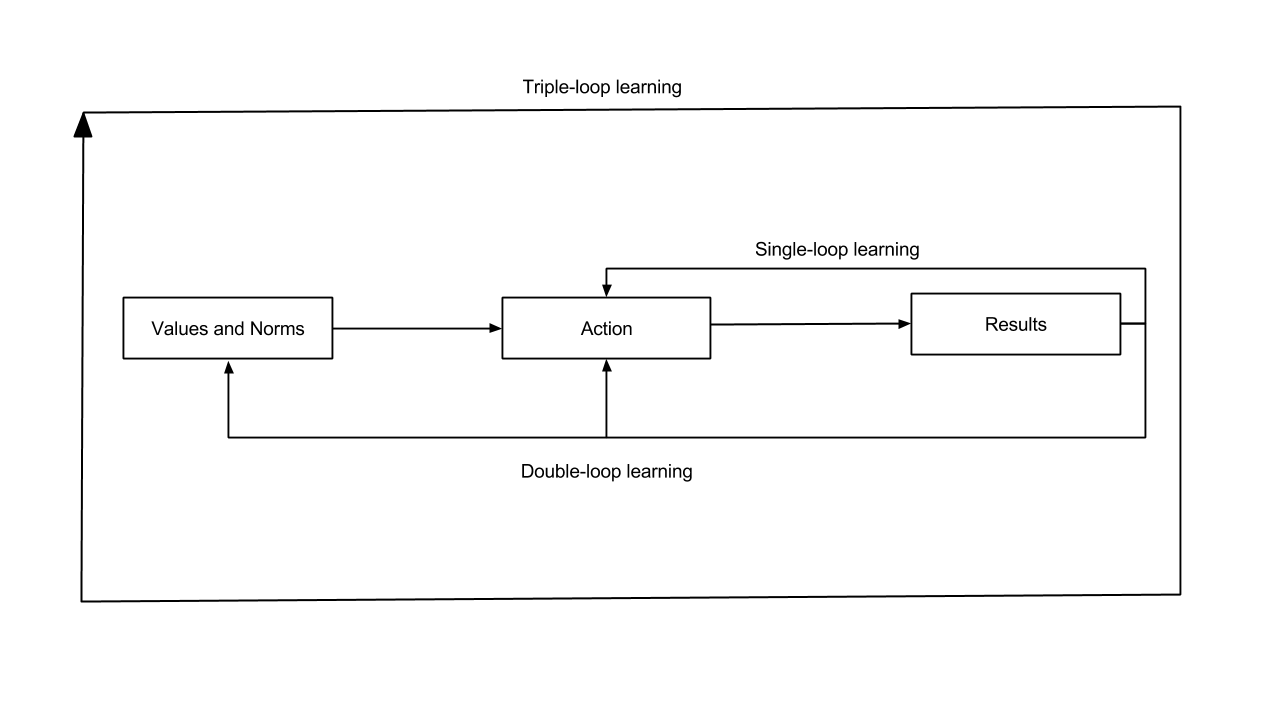
\includegraphics[width=\textwidth, keepaspectratio]{figures/triple-loop.png}
	\caption{Triple-loop learning.}
	\label{figure:triple-loop}
\end{figure}

\clearpage

\section{Shared Mental Models}

The theory of shared mental models is from cognitive psychology, and can be used as a lens to evaluate agile development and methodology as described by Petter et al\cite{Petter2013}. The concept is that a team has a shared mental model that is central to the mutual understanding between team members, and thus essential to project success. Without a good shared mental model a team is left with a poor understanding of the task at hand, as well as barriers for cooperation. Two metrics used to measure a team's shared mental model are ``similarity'' and ``accuracy''. Where ``similarity'' is the degree which the shared mental model is similar between team members, and ``accuracy'' is the degree which the shared mental model matches objective measures. 

\subsection{The stages of Shared Mental Model generating}

	
Four different stages of building shared mental models are identified \cite{Petter2013}. These are knowing, learning, understanding and executing. An overview of these stages is seen in  \autoref{table:stages-mental-model}. Knowing is the stage where a team gets exposed to information relating to their project and project goals, at this stage team members are encouraged to share information between each other. The second stage is the learning stage, this stage consists processing the information gained in the knowing stage. The understanding stage is defined by reaching consensus and understanding the team member's individual views. Executing is the last stage, with a developed shared understanding the team is able to reach goal, at this stage a team responds to a situation based on the work done in the previous stages.

\begin{table}[!h]
	\begin{centering}
	\caption{Four stages of mental model building}
	\label{table:stages-mental-model}
	\begin{tabular}{l | p{0.7\textwidth}}

	\hline
	Stage & Description \\
	\hline
	Knowing &  Information exposure and sharing\\
	Learning & Information processing \\
	Understanding & Consensus and common ground \\
	Executing & Shared understanding and  \\
	\hline
	
\end{tabular}
\end{centering}
\end{table}

	
\subsection{Shared Mental Models and retrospectives}

Petter et. al. \cite{Petter2013} describe multiple agile development practices, but do not focus a lot on the agile retrospective. In the appendix of the article they give the following link between retrospectives and shared mental models.

\begin{quote}
Enhances the development of learning and understanding stages by facilitating the information sharing and integration. This practice also improves the teams’ executing capability in the next sprint
\end{quote}

The shared mental model practices that are involved in the retrospective are identified as self corrective, training and reflectivity. We discuss this phenomenon more in \todo[inline]{Link til discussion del om SMM og Retro} 


\todo[inline]{skriv om retro og SMM (står i slutten av arikkelen)}


\clearpage


\chapter{Method}

In this chapter we will describe the environment and motivation for our research. We will also explain the process for this study.

\section{Research Goal}
After over a decade of agile development where retrospectives have been recommended as a practice that should introduce improvements in development practices, the outcome of the retrospective is still undetermined. We will investigate this, focusing on the organizational learning that happens through retrospectives and the characteristics of the retrospective. When we say characteristics of the retrospective we will investigate the output of conducting retrospectives, the processes used and the impediments that faces the retrospective. We will investigate these characteristics in the context of existing academic work. \textit{Our goal for this study is to investigate the outcome returned from the retrospective in terms of organizational learning and retrospective characteristics.} Elaborating on this goal we get two sub-goals: 

\begin{enumerate}
	\item What are the main characteristics in current retrospective practices, in terms of outcome, processes and impediments? 
	\item How is learning achieved through current retrospective practices, in light of organizational learning theory? 
\end{enumerate}

The first sub-goal relates to the characteristics of the retrospective. We will throughout this study investigate and describe which characteristics are current in todays retrospective. We will focus on the output, the processes used and the impediments. When we say output we will investigate what improvement opportunities are created, which improvements are actually implemented and how the enthusiasm evolves as a result of the retrospective. We will also investigate the processes used by practitioners of the retrospective and the impediments that hinder them from returning value. 

The second sub-goal will investigate the learning achieved through the retrospective practice. We will employ the learning theory described by Argyris and Schön \cite{Argyris1996} and compare the governing values of Model I and Model II against the results we see from our case studies. We will also investigate which types of learning, single-, double-, or triple-loop, occur through the retrospective practice. 

\section{Research Design}
For this study we will conduct a multiple-case study to investigate our research goal. It will consist of one depth study and one breadth study. We describe each of these in short in this section and following in the chapter we will elaborate on these. A short summary of the research design can be seen in \autoref{table:research-design}. 

Our first case study is a depth study investigating the long-term practice of one retrospective practicing agile development team. This will be done through analyzing a set of retrospective reports using tabulations and then reflect on the results together with the team. 

The second case study is a breadth study investigating the retrospective practices of other teams. This will be done interviewing representatives from different retrospective practicing teams.

Our analysis method consists of two parts. The first part is a descriptive discussion on the results found during the two case studies that focuses on the characteristics of the retrospective practice. The second analysis method is comparing our results against the organizational learning framework created by Argyris and Schön \cite{Argyris1996} specifically the governing values of Model I and Model II. 

\begin{table}[!h]
	\begin{center}
	\caption{Research design for this multiple-case study.}
	\label{table:research-design}
	\makebox[\textwidth]{%
		\begin{tabular}{l p{0.7\textwidth}}
		\hline
		\textit{Step} & \textit{Description} \\
		\hline
		\textbf{Case 1} & Depth Study \\
		Content Analysis & Tabulation Analysis of Retrospective Reports \\
		Feedback Sessions & Reflection with team about the results of the content analysis. \\[12pt]
		\textbf{Case 2} & Breadth Study \\
		Interview Sessions & Interview different teams \\[12pt]
		\textbf{Analysis Method} & \\
		Characteristics & Descriptive Discussion on Results \\
		Organizational learning & Compare results against Argyris and Schön's \cite{Argyris1996} governing values. \\
		\hline
		\end{tabular}
	}
\end{center}
\end{table}

\section{Depth Study}
Our depth study consisted of two steps. The first step was to perform a content analysis on earlier retrospective reports. The second step was to hold several feedback sessions with the team reflecting on the results of the content analysis. We will describe each of these steps further in the following subsections.

\subsection{Content Analysis}

\subsubsection{Data Material - Retrospective Reports}
Through our supervisor we were put in contact with an experienced team in Norway. The team, which we will refer to as team Zulu is described more closely in \autoref{section:team-zulu-description}, graciously allowed us access to their retrospective logs, for us to analyze.

The retrospectives consisted of five different sections being: Where and What, Actions, Comments, Signatures and Case Proceedings, as can be seen in \autoref{table:retrospective-format}. 
The ``Where and What'' section contained general data about the retrospective such as the date, iteration dates, iteration number, contact person and other general information. ``Actions'' described the improvement actions that had resulted from the retrospective. It contained a description for each action, who is responsible for that action, deadline, status and comments from the participants. The ``Comments'' section contained comments, if any, from the participants of the retrospective if they had any specific input for the retrospective in general. ``Signatures'' contained the signature for each participant in the retrospective. The last section,``Case Proceedings'' contained information about the changes in the document and circulation of it.

\begin{table}[!h]
	\begin{center}
	\caption{The section of the retrospectives}
	\label{table:retrospective-format}
	\makebox[\textwidth]{%
		\begin{tabular}{l | p{0.7\textwidth}}
		\hline
		Part & Description \\
		\hline
		Where and What & Containing general data about the retrospective such as date, iteration location, etc. \\
		Actions & Describes the actions resulting from the retrospective it also includes data on responsible person, deadline etc. \\
		Comments & General comments from the participants for the retrospectives. \\
		Signatures & The signatures from each participant participating in the retrospective. \\
		Case Proceedings & The changelog and circulation of the retrospective. \\
		\hline
		\end{tabular}
	}
\end{center}
\end{table}

While getting familiar with the retrospectives we found that the only section containing any value in the terms of organizational learning was the actions described in the ``Action'' section. In most of the retrospective reports multiple actions were described relating to different issues observed during the iteration. The format of the actions can be seen in \autoref{table:action-format}. 

\begin{table}[!h]
	\begin{center}
	\caption{An generic example of an action provided in the retrospectives.}
	\label{table:action-format}
	\makebox[\textwidth]{%
		\begin{tabular}{| l  p{0.5\textwidth} |}
		\hline
		Action x &  \\
		Deadline & 01.01.2015 \\
		Action description & Always add a week to the iterations during holidays. \\
		Comments & Resources are not reliable during holidays. \\
		Responsible unit & Team X \\
		User responsible for action & John Smith \\
		Status & Completed or In Process \\
		Completed & 31.01.2014 \\
		Type & Preventive or Corrective \\
		\hline
		\end{tabular}
	}
\end{center}
\end{table}

\subsubsection{Analysis Method}
\label{analysis-method}
To retrieve any research-worthy knowledge from the actions given by the retrospective reports we needed means compare them. We settled on tabulations as our analysis method for the actions. Tabulations provide easy means of rendering data comprehensible. Krippendorff ~\cite{Krippendorff2004} describes tabulations as: 

\begin{quote}
Tabulation refers to collecting same or similar recording units in categories and presenting counts of how many instances are found in each. Tabulations produce tables of absolute frequencies, such as the number of words in each category occurring in a body of text, or of relative frequencies, such as percentages expressed relative to the sample size, proportions of a total, or probabilities.
\end{quote}

For our case we are going to use absolute frequencies to count the occurrences of different categories. Using relative frequencies would not suffice in our case where determining whether an action is twenty percent technical and eighty percent procedural or thirty percent technical and seventy percent procedural would be immensely difficult and not to mention impractical. Rather an action could be neither technical or procedural, be one of them, or be both. Thus resulting in us using absolute frequencies when we are counting occurrences of the different categories. 

To determine what the categories should be we conducted a pilot analysis that can be read about in Appendix \autoref{pilot-analysis}. The final result of categories were agreed upon by the team and are shown in \autoref{table:content-analysis-categories}. It consisted of six main themes: Nature, Context, Decision Making, Organizational Learning, Development and Collaboration. Nature, Context, Decision Making, Development and Collaboration can be related to the characteristics and output of retrospective practices. The organizational learning theme relates directly to the learning output and the team organizational learning of the practice. Each of the six themes had several categories which an action would be put in. These categories are shown in \autoref{table:content-analysis-categories} and are further described and defined in Appendix \autoref{appendix:categories}. 

\begin{table}[h]
	\begin{center}
		\caption{The final set of themes and categories that the content analysis is based upon.}
		\label{table:content-analysis-categories}
		\begin{adjustbox}{width=\textwidth, totalheight=0.9\textheight, keepaspectratio}
			\begin{tabular}{| l | l | p{0.5\textwidth} |}
			\hline
			Theme & Category & Short Description  \\
			\hline
			Nature & Positive & If an action is a result of a continuation of a process \\ \cline{2-3}
			& Negative & Action is a result of a arisen problem \\ \cline{2-3}
			& Undefined & The nature of the action is unclear or undefined \\ \hline
			Context & Technical & If the action is related to some technical context. \\ \cline{2-3}
			& Process & Action is related to a process context \\ \cline{2-3}
			& Undefined & The action could not be related to either technical or process \\ 
			\hline
			Decision Making & Strategic & Action is suggesting long-term change \\ \cline{2-3}
			& Tactical & The action is related to identification and use of resources. \\ \cline{2-3}
			& Operational & If the action is ensuring effectiveness and day-to-day operations \\ \cline{2-3}
			& Undefined & If the action is unclear and doesn't fit any of the other decision making categories. \\ 
			\hline 
			Organizational learning & Single-loop & If the action do a change that only influence the effects \\ \cline{2-3}
			& Double-loop & If one understand the factors that influence effects, and the nature of this influence. \\ \cline{2-3}
			& Undefined & If the action unclear in terms of organizational learning \\ \hline
			Development Phase & Development & Action is related to the development phase \\ \cline{2-3}
			& Testing & The action is related to testing \\ \cline{2-3}
			& Documentation & Action is related to Documentation \\ \cline{2-3}
			& Builds & The action is related to building of software systems \\ \cline{2-3}
			& Release & The action is related to releasing of software \\ \cline{2-3}
			& Business & The action is related to business development \\ \cline{2-3}
			& Undefined & The action is not related to any of the development phases described above \\ 
			\hline
			Collaboration & Communication & Related to communication within a team \\ \cline{2-3}
			& Leadership & Action is related to leadership \\ \cline{2-3}
			& Competence & Action is a result of lacking knowledge or experience \\ \cline{2-3}
			& External relations & The action is related to customer relations or other external stakeholders \\ \cline{2-3}
			& Planning & The action is a result of bad or good planning \\ \cline{2-3}
			& Undefined & Action is not related to any of the collaboration issues \\
			\hline
			\end{tabular}
		\end{adjustbox}
	\end{center}
\end{table}

In addition using tabulations for analyzing the actions, we investigated recurring issues. A retrospective is intended to highlight issues and potential actions that can be taken to correct or improve the issues. However it is not necessarily the case that every action is implemented as intended, or in the time frame originally intended. As such issues might come up again and again. Being able to identify these long term issues and address them before they become reoccurring is a clear potential improvement for a team or an organization. Therefore it is of great interest to identify these issues in our analysis. We will be looking through the available information and noting if an issue arises multiple times over time. Also of interest are unresolved issues, which are issues that are raised and a corrective action is agreed upon, but the action is either not implemented or implemented fully.

\paragraph{Processing Steps}
To perform our content analysis we first defined a set of processing steps that both authors were to follow. All the processing steps can be seen in \autoref{table:content-analysis-steps}.

\begin{table}
	\begin{centering}
		\caption{Description of the content analysis steps.}
		\label{table:content-analysis-steps}
		\begin{tabular}{l p{0.8\textwidth}}
			Step & Description \\ 
			\hline
			1 & Specify and document all the tabulation categories. \\
			2 & Send analysis documentation to the case participants to get feedback on the analysis measurements. \\
			3 & Create a spreadsheet for each author containing data on all the categories and all the actions. \\
			4 & Each author read through all the retrospectives separately, setting marks for each category that an action fits in. \\
			5 & When both authors were finished reading through all the retrospective they compared the results and put everything into a combined spreadsheet. If the authors disagreed on their markings a short discussion would commence and one would try to find an agreement. If an agreement could not be found the authors would turn to other external researchers to help identify the correct solution. \\
			6 & The content analysis was finished when all the actions were in the combined spreadsheet. \\
		\end{tabular}
	\end{centering}
\end{table}

The first step was to specify all the tabulation categories that were going to be included in the content analysis. Once all the categories were found and specified we documented them to ensure both authors had the same understanding of what each category meant. 

When the categories had been documented we sent them to the case participants to get feedback on the analysis measurements and verify that it was not anything that we had overlooked that the participants would like answers to. 

Once the feedback was incorporated into the content analysis we created a spreadsheet containing all the actions along the top row and all the categories along the first column. We created one spreadsheet for each author and one extra that would later be used for comparison. 

When the spreadsheets were done the next step was analyzing all the actions. Each author, separately, read through all the retrospectives and for each action marked which categories it belonged to. Each action could belong to several categories for an example an action could belong to both Testing and Documentation. For each of the six themes at least one mark had to be put down, and the maximum marks would be the number of categories in that theme. 

After all the retrospectives were read through and every action was tabulated the authors compared their results. For each action the authors would compare all the marks set for that action and if they both agreed upon all the marks the action would be copied to a new spreadsheet. If the authors disagreed they would go back to the action read it once more and try to find a classification that both could agree to. If this turned impossible we would seek advice from external researchers to gain a suitable solution. 

Once all the actions were compared and all the actions were in the new spreadsheet the content analysis was finished and data could then later be extracted from the spreadsheets. 
\afterpage{\clearpage}
\subsubsection{Content Analysis Limitations}
In this subsection we will describe the challenges and limitations of our content analysis from the 77 retrospectives. Mainly there were two challenges that occurred during our content analysis, missing contexts and borderline actions. Each is described in detail below. 
\paragraph{Missing Contexts}
As the retrospectives we were given mostly contained actions that resulted from the retrospective meetings, context of how the actions were brought to light could sometimes be missing. In those cases the actions either could have come from a problem happening during the iteration, a new idea that was put forth during the iteration or something similar. As some of the actions lacked context we included the undefined category to each theme so that in the cases were we could not tell whether an action was in a concrete development phase, or another theme, we could put it in undefined. 
\paragraph{Borderline Actions}
Borderline actions were the second challenge while performing our content analysis. An example is the action: 
\begin{quote}
To improve the understanding of the processes, the workflow diagrams and the other relevant documentation should be copied to the WIKI.
\end{quote}
This action could either be understood as ``The workflow diagrams and other relevant documentation is so good that we should put it on the WIKI'' or ``People do not have enough understanding of the processes and we should give them more documentation''. The first option could be classified as a positive action as the working documentation is good and should be used more, while the second option would be classified as a negative action as it is a problem that the understanding of the processes is not good enough. This action would be classified as undefined in our analysis as it both requires more context and as it lacks the context can be a borderline action between positive and negative. 

To deal with the borderline actions we added the steps of each author doing a separate analysis before comparing with the other author to identify the borderlines and find a adequate classification for them.

\subsection{Feedback Sessions}
As the final part of the first case-study several feedback sessions were held, to gather valuable input from the team and their reflections on the analysis. Each of these feedback session will be described in the following subsections. 

\subsubsection{Feedback Session: Team Discussion}
For the first feedback session we visited the team in person and held a presentation followed by a group discussion. The presentation was held in a meeting room in front of the team. The concept of the analysis was first explained and discussed with the team members, in order to ensure that there existed a common understanding of the work being presented. The presentation was also simultaneously a dialog between the presenters and the team. This was facilitated by constantly asking questions and encouraging discussion. One of the ways of encouraging discussion was to ask the team ``What expectations do you have for this category?'' before showing the results of the analysis. This ensured that we got their speculation as well as their reaction to the analysis. 

\subsubsection{Feedback Session: SCRUM Master Interview}
The second feedback session we had was an interview with the SCRUM master of the team. We spent a short while preparing and reviewing the questions we had prepared. The interview would be held in a semi-structured manner with the goal of having an open discussion of the results of the team discussion as well as gaining insight on the themes of the analysis. During the interview notes were taken, as well as recorded, and the SCRUM master was encouraged to speak his mind on relevant subjects. 

\subsubsection{Feedback Session: Team Leader}
The third feedback session was an interview where we presented additional findings, based on the results from the former feedback sessions and discussed the impact on the team. The interview was conducted with voice chat with the leader of the team. The session also served as a brainstorming session for the team leader in order to prepare a retrospective evaluation session he would lead the following week. This evaluation session would be a discussion between all members of the team where they discussed the current state of the retrospective after the feedback session and analysis.

\subsubsection{Feedback Session: Internal Team Evaluation}
The last session was conducted by the team internally without the authors present. The team had a ``Meta-Retrospective'' where they discussed the current state of the retrospective sessions, as well as their thoughts on the first feedback session. The team held the session as a normal retrospective, but with a semi-structured agenda that the team leader had developed in cooperation with the authors. The team leader then sent the meeting log to us, and had a short interview explaining the content.

\section{Breadth Study}
Our second case-study aimed to get a broader picture of the practices used for retrospectives today. We decided on a semi-structured interview, in order to be free to improvise as well as being prepared to ask stimulating questions to the interview subject.

\subsection{Semi-structured interviews}
We decided to use a semi-structured interview as our model for the interviews. An unstructured, or semi-structured does not have a complete script, and leaves room for improvisation, unlike a structured interview where there is a complete script. \cite{Myers2007} This approach was chosen to leave the interview subject free the elaborate on subjects they found interesting. 

A list of questions was prepared in order to serve as a guideline for the interview. This interview guide was divided into four sections, relevant for our research, being: ``General overview'', ``Team dynamics'', ``Organizational learning'' and ``Anything else''. A short description of each of these are shown in \autoref{table:interview-guide-overview}. The complete interview guide including all the questions can be found in appendix \autoref{section:interview-guide}. These four sections were chosen due to experiences working with team Zulu, as well as through a discussion with our supervisor. 

\begin{table}
	\begin{centering}
	\caption{Interview guide overview}
	\label{table:interview-guide-overview}
	\begin{tabular}{l p{0.8\textwidth}}
	 	Step & Description \\ 
		\hline
		General overview & Questions relating to the holding of the retrospective and learning\\
		Team dynamics & Questions on how team dynamics are handled and how they are experienced in the team \\
		Organization learning & Questions on how the team approach learning \\
		Anything else & Summary questions intended to cover potentially missed topics \\
	\end{tabular}
	\end{centering}
\end{table}

In order to conduct a successful semi-structured interview Myers and and Newman mentions several factors that need to be acknowledged \cite{Myers2007}. Among these are the lack of trust, elite bias and ambiguity of language. In order to avoid these potential pitfalls we spent time ensuring a mutual understanding and respect with the interview subject, for example by explaining our intentions and maintaining a friendly tone during the interview. 

The interviews were if possible held in person or over voice chat. This was done to lower the barrier for dialog as much as possible and let the interviewee speak as easily as possible. However at one point one interviewee had to resort to mail due to time constraints, we decided to keep the interview and the answers are included in the appendix. 

\subsection{Interview Subjects}
\label{subsec:Interview-Subjects}
In order to select interview subjects within the industry we contacted potential practitioners through e-mail or phone. As well as consulting our advisors. We wanted subjects with experience both holding and participating in retrospectives in order to gain multiple views of the retrospective experience. The base criteria was that participants had to be a part of a team that conducts retrospectives on a regular basis. We wanted a varied spread for the interview subjects and selected subjects based on their project and team compositions. Consultants, distributed teams, product development teams, small teams and big teams were some of the considerations for teams we wanted for this study.

\section{Analysis Method}
Our analysis method consisted of several steps. After gathering all the data from content analysis, feedback sessions and interviews each researcher went through the material separately. For the feedback sessions and interviews we listened through the recordings taking notes ensuring nothing was missed during the sessions. After all the material was worked through we compared the different data against each other and against earlier academic work. The academic fields used is: Retrospective literature and organizational learning. The fields was chosen as retrospectives is a shared learning activity and thus organizational learning is useful to see how the team as a whole learns and retrospective literature  as it can be used to compare the characteristics for retrospective practices.

\begin{figure}[!h]
	\centering
	\includegraphics[height=0.5\textheight, keepaspectratio]{figures/analysis.png}
	\caption{A picture of our whiteboard during analysis}
	\label{fig:Analysis-trends}
\end{figure}

\clearpage

\section{Participants}
Our research bases itself on the primary data gathering methods: Retrospective depth analysis of one team and interview input from other teams. In this section we will present the participants using the phonetic alphabet as identifiers. Many of the participants were recruited from existing research projects being ``Agile 2.0'' and ``SMIGLO''.

\subsection{Depth Analysis Participant - Team Zulu}
\label{section:team-zulu-description}
Team Zulu is situated in Norway and develop a human resource system. The team has been working with agile principles for over 10 years. An overview of the team can be seen in \autoref{list:team-zulu}

 \begin{enumerate}
 \label{list:team-zulu}
	\item 1 HoD – Product Owner 
	\item 1 SCRUM Master
	\item 1 Architect
	\item 4 Developers
	\item 1 Content Responsible
	\item 2 Testers
	\item 1 Build and DB responsible
	\item 1 Third line support engineer
\end{enumerate} 

\subsection{Breadth Study Participants}
In this section it is a short description of each interview subject. All participants in the interview research were familiar with retrospectives, and agile development practices. The selection process is described in \autoref{subsec:Interview-Subjects} and an overview of the team and representatives can be found in \autoref{table:participants}

\subsubsection{Team Alfa}
Team Alfa consisted of 22 members and we spoke to two of them. The project leader and one developer. The team consisted of designers, testers, front-end developers and back-end developers who all worked with media solutions for a customer. 

\subsubsection{Team Bravo}
Team Bravo consisted of 6 members, 2 in Norway, 3 developers in Poland and 1 tester in Shanghai. The project leader and Scrum master were in Norway. 

\subsubsection{Team Charlie}
From team Charlie we spoke to one representative. The participant was project coordinator, project leader and SCRUM master for a development team consisting of four persons. The participant also had responsibility for agile practices in his company which develops HR solutions. 

\subsubsection{Team Delta}
The representative for Team Delta was a developer and the teams SCRUM master. The team developed HR solutions. 

\subsubsection{Team Echo}
The participant from team Echo was a consultant acting as a developer and semi-project leader for a multi-platform development project. The team consisted of 10 members and developed four different products for one customer.

\subsubsection{Team Foxtrot}
Team Foxtrot consisted of about 20 members in the roles of design, ux, front-end, back-end and project leaders. The representative from team Foxtrot was a system developer and he chose to responded to our interview through email. We acknowledge that this might have a resulted in input getting lost. However the input that has been gathered will still be able to give us some data which can be used for this study. 

\subsubsection{Team Golf}
Team Golf consisted of 2 members working in Norway, with the rest of the team situated in Shanghai. The representative from Team Golf was the SCRUM master for the team. 

\begin{table}[!h]
	\begin{center}
	\caption{Table overview over interview participants}
	\label{table:participants}
	\begin{tabular}{l p{0.5\textwidth} l}
	\hline
	Team & Description & eRpresentatives\\
	\hline
	Alfa & Project leader & 2 \\
	& Developer & \\
	Bravo & SCRUM Master & 1  \\
	Charlie & SCRUM master, project leader and coordinator & 1 \\
	Delta & Developer and SCRUM master & 1 \\
	Echo & Developer and project leader & 1 \\
	Foxtrot & System Developer & 1 \\
	Golf & SCRUM Master & 1 \\
	\hline
	\end{tabular}
	\end{center}
\end{table}

\clearpage
\chapter{Results}
\todo[inline]{Some intro to the chapter}

\clearpage
\section{Content Analysis Results}
From the retrospective reports we obtained several interesting results. We will go through each of them below starting with some key numbers and then move on to the results of the content analysis. Then we identify some trends observed while performing the content analysis. 

\subsection{Key Numbers}
In this section we will present some key numbers of the retrospective results and these numbers can also be seen in \autoref{table:key-numbers}.The retrospective reports spanned over a period of five years from August 2009 to November 2014. This amounts to 278 weeks and we are going to refer to week numbers from the first retrospective for the remainder of this report. 
\begin{table}[!h]
	\begin{center}
	\caption{Some key numbers from the retrospectives}
	\label{table:key-numbers}
	\makebox[\textwidth]{%
		\begin{tabular}{ l | p{0.5\textwidth}}
		\hline
		Key-value & Value  \\
		\hline
		Retrospective report period & 278 Weeks \\
		Number of total actions & 343 \\
		Number of unresolved actions & 65 \\
		Average actions per week & 1.23 \\
		Average unresolved action per week & 0.23 \\
		\hline
		\end{tabular}
	}
\end{center}
\end{table}
During the 278 weeks 77 retrospectives were held and and within these 343 actions was created, where 65 of these actions were still unresolved. This yields an average of 4.45 actions per retrospective and 0.84 unresolved per retrospective. This is equal to 1.23 actions per week, where one have 0.23 unresolved actions per week. 

In \autoref{figure:key-numbers} we can see the development of numbers of actions. We can see that the team has had a pretty steady amount of actions with no abnormal spikes or changes until week 180. The total amount of actions follows the average expected actions quite close and reveals the steady number of actions.
At week 180 a slight increase in the number of actions begins. This lasts until until 237 when the amount of actions per retrospective starts to even out. 
The amount of active (or unresolved) actions has a steady amount of total actions increasing at about the same rate as the total number of actions. 


\begin{figure}[!h]
	\centering
	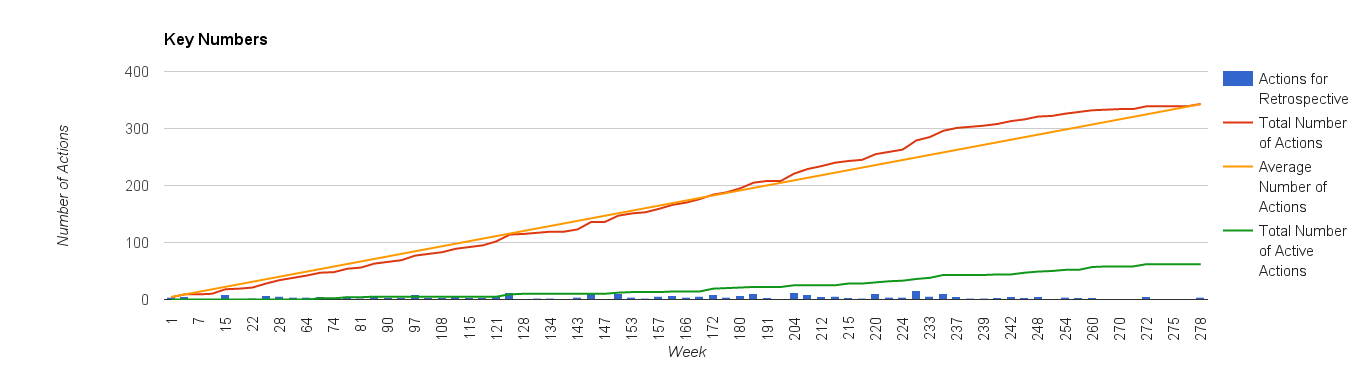
\includegraphics[width=\textwidth, keepaspectratio]{figures/key-numbers.png}
	\caption{A visual representation of some of the key numbers.}
	\label{figure:key-numbers}
\end{figure}
\clearpage	

\subsection{Analysis Results}
In this section we will present the results from our content analysis. We will present the results for each theme defined in \autoref{method:categories}. 

\subsubsection{Nature}
The content analysis revealed that most actions are created as a result of negative problems that has occurred during the development. 89.3\% of the actions were negative, while 5.5\% of the actions were positive and acknowledged good working practices that would be continued. 5.2\% of the actions we lacked the context to determine whether they were positive or negative. As for the distribution of the actions over each retrospective there was no abnormalities except week 97 where there was an unusual amount of positive actions. However while looking into this week we found nothing in particular that could be identified as cause for this spike. As can be seen in \autoref{figure:nature-pa} and \autoref{table:nature-results} the classification of the active actions pretty much mirrored the results from the total actions. 

\begin{table}[!h]
	\begin{center}
	\caption{Analysis results from the content analysis for the nature of the action.}
	\label{table:nature-results}
	\makebox[\textwidth]{%
		\begin{tabular}{| l | l | l | l | l |}
		\hline
		Category & \multicolumn{2}{|c|}{All Actions} & \multicolumn{2}{|c|}{Active Actions}  \\
		\cline{2-5}
		& Number & Percentage & Number & Percentage \\	
		\hline
		Positive & 19 & 5.5\% & 1 & 1.6\% \\
		Negative & 310 & 89.3\% & 57 & 90.5\% \\
		Undefined & 18 & 5.2\% & 5 & 7.9\% \\
		\hline
		\end{tabular}
	}
	\end{center}
\end{table}

\begin{figure}[!h]
	\centering
	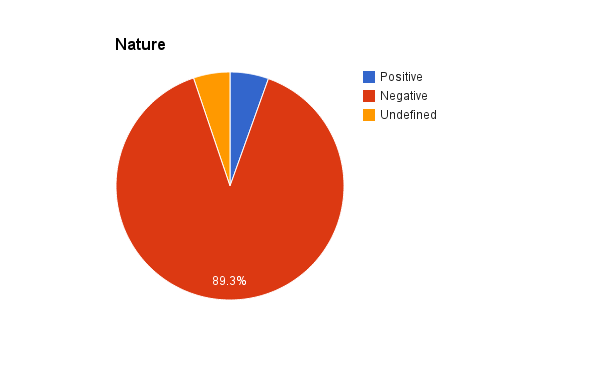
\includegraphics[width=\textwidth, keepaspectratio]{figures/nature-p.png}
	\caption{The negative, positive and undefined distribution of all the actions.}
	\label{figure:nature-p}
\end{figure}

\begin{figure}[!h]
	\centering
	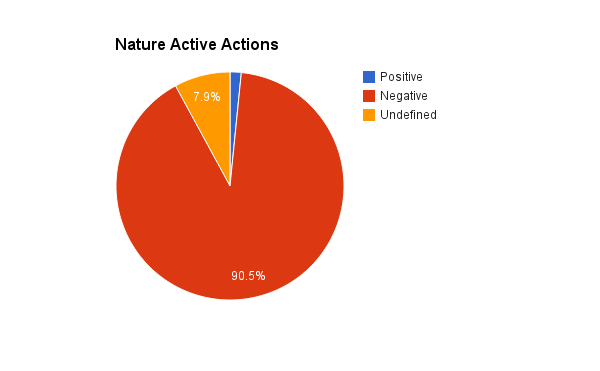
\includegraphics[width=\textwidth, keepaspectratio]{figures/nature-pa.png}
	\caption{The negative, positive and undefined distribution of the active actions.}
	\label{figure:nature-pa}
\end{figure}

\begin{sidewaysfigure}[!h]
	\centering
	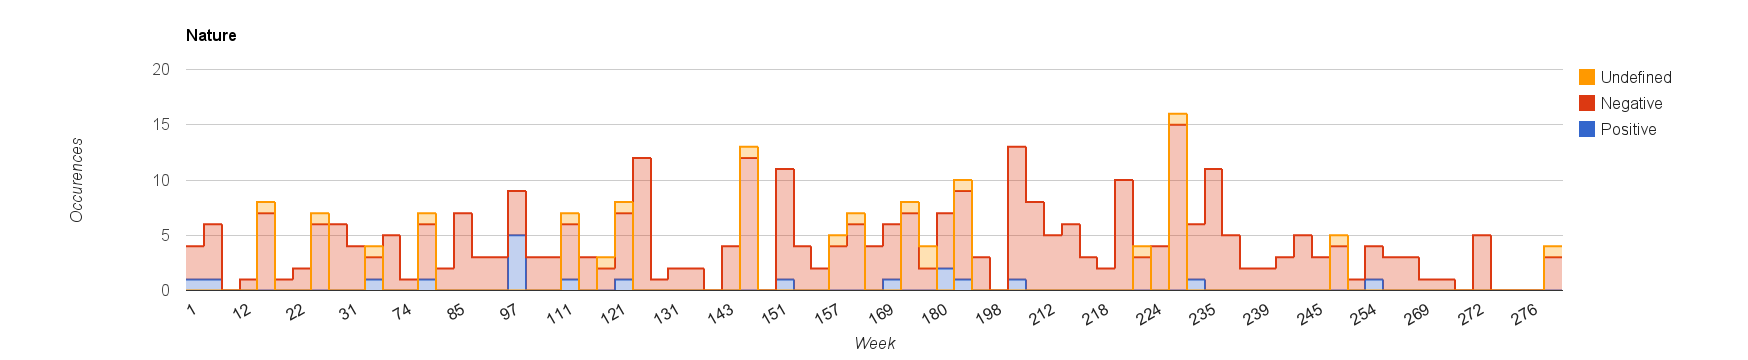
\includegraphics[width=\textwidth, keepaspectratio]{figures/nature-l.png}
	\caption{The distribution of negative, positive and undefined actions across the timespan}
	\label{figure:nature-l}
\end{sidewaysfigure}

\clearpage

\subsubsection{Context}
For the context of the actions analyzed mostly where process related ones. The process actions numbered in 228, which is equal to 58.6\% of all the actions. The Technical ones numbered as 157 which is 40.4\%, while only 4 actions were undefined which results in 1\% of the total actions. As for the distribution over the timespand analyzed there where no abnormalities as can be seen in \autoref{figure:context-l}. For the active actions the results become more equal as seen in \autoref{figure:context-pa}. However it is worth mentioning that the active actions are a sub-group of the total and thus this result is probably a skewed grouping. 

\begin{table}[!h]
	\begin{center}
	\caption{Analysis results from the content analysis for the context of the action.}
	\label{table:context-results}
	\makebox[\textwidth]{%
		\begin{tabular}{| l | l | l | l | l |}
		\hline
		Category & \multicolumn{2}{|c|}{All Actions} & \multicolumn{2}{|c|}{Active Actions}  \\
		\cline{2-5}
		& Number & Percentage & Number & Percentage \\	
		\hline
		Technical & 157 & 40.4\% & 37 & 52.1\% \\
		Process & 228 & 58.6\% & 34 & 47.9\% \\
		Undefined & 4 & 1\% & 0 & 0\% \\
		\hline
		\end{tabular}
	}
	\end{center}
\end{table}

\begin{figure}[!h]
	\centering
	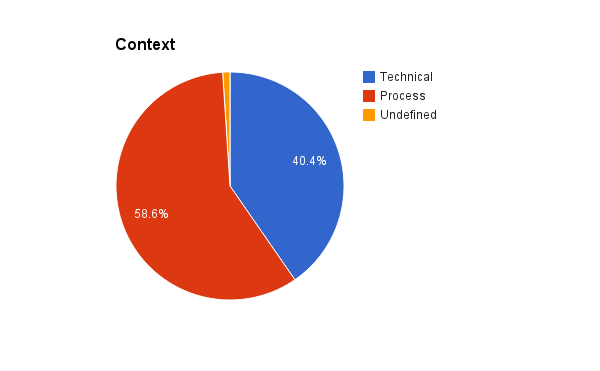
\includegraphics[width=\textwidth, keepaspectratio]{figures/context-p.png}
	\caption{The distribution of technical, process and undefined related actions.}
	\label{figure:context-p}
\end{figure}

\begin{figure}[!h]
	\centering
	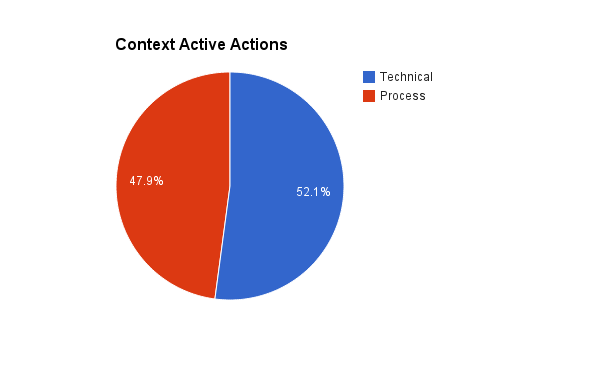
\includegraphics[width=\textwidth, keepaspectratio]{figures/context-pa.png}
	\caption{The distribution of technical, process and undefined related actions over.}
	\label{figure:context-pa}
\end{figure}

\begin{sidewaysfigure}[!h]
	\centering
	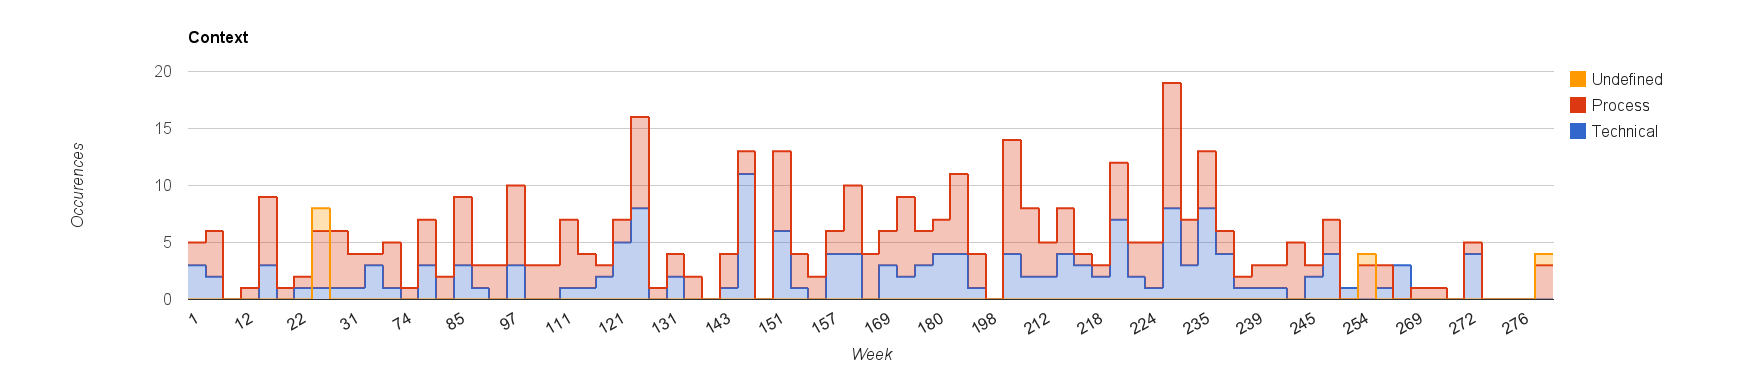
\includegraphics[width=\textwidth, keepaspectratio]{figures/context-l.png}
	\caption{The distribution of technical, process and undefined related actions across the timespan.}
	\label{figure:context-l}
\end{sidewaysfigure}

\clearpage

\subsubsection{Decision Making}
The decision making results showed that the operational decision occurred most in the actions as can be seen in \autoref{table:decision-making-results} and \autoref{figure:decision-p}. Operational decisions occurred in 53.2\% of the actions, while tactical was at 25.9\% and strategic was at 16.1\% of the actions. There only was four cases where we were not able to determine which kinds of decision making type it was. For the distribution over time, as shown in \autoref{figure:decision-l}, there was no emerging patterns and all the decision making types was evenly distributed. The active actions mirrored the total actions almost equal as can be seen in \autoref{figure:decision-p} and \autoref{figure:decision-pa}.

\begin{table}[!h]
	\begin{center}
	\caption{Analysis results from the content analysis for the decision making perspective of the action.}
	\label{table:decision-making-results}
	\makebox[\textwidth]{%
		\begin{tabular}{| l | l | l | l | l |}
		\hline
		Category & \multicolumn{2}{|c|}{All Actions} & \multicolumn{2}{|c|}{Active Actions}  \\
		\cline{2-5}
		& Number & Percentage & Number & Percentage \\	
		\hline
		Strategic & 55 & 16\% & 10 & 16.1\% \\
		Tactical & 89 & 25.9\% & 18 & 29\% \\
		Operational & 195 & 56.9\% & 33 & 53.2\% \\
		Undefined & 4 & 1.2\% & 1 & 1.6\% \\
		\hline
		\end{tabular}
	}
	\end{center}
\end{table}

\begin{figure}[!h]
	\centering
	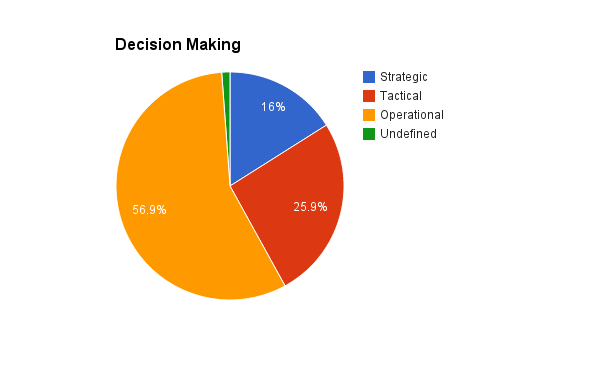
\includegraphics[width=\textwidth, keepaspectratio]{figures/decision-p.png}
	\caption{The distribution of different decision making decisions as they occurred over all the actions.}
	\label{figure:decision-p}
\end{figure}

\begin{figure}[!h]
	\centering
	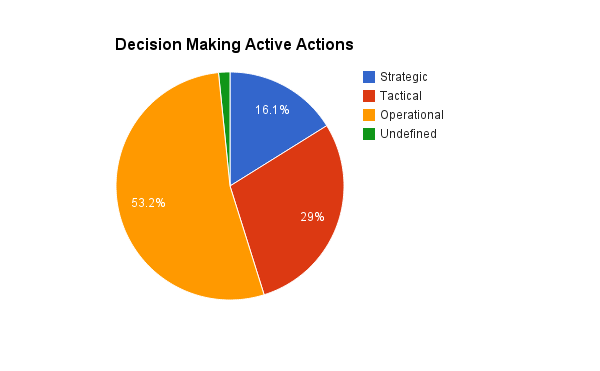
\includegraphics[width=\textwidth, keepaspectratio]{figures/decision-pa.png}
	\caption{The distribution of different decision making decisions as they occurred over the active actions.}
	\label{figure:decision-pa}
\end{figure}

\begin{sidewaysfigure}[!h]
	\centering
	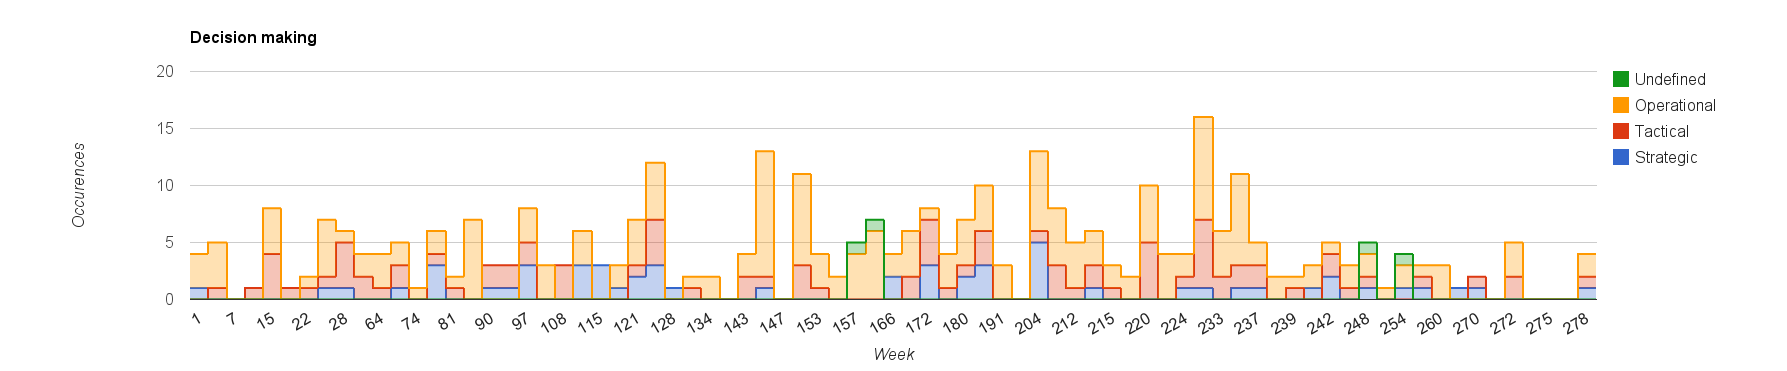
\includegraphics[width=\textwidth, keepaspectratio]{figures/decision-l.png}
	\caption{A timeline showing the distribution of the different decision making decisions for all the actions.}
	\label{figure:decision-l}
\end{sidewaysfigure}
\clearpage

\subsubsection{Organizational Learning}
In terms of organizational learning each action could be defined as single-loop, double-loop or undefined. The results yielded from the content analysis showed that single-loop was the most occurring type of organizational learning with 66.4\% of the actions. Double-loop had 27.2\% of actions, and the rest was undefined at 6.4\%. The distribution over the timespan, \autoref{figure:learning-l} of the analysis showed that the three categories was evenly distributed. The active actions was very similar to the total amount of actions and only had some small negligible variances as can be seen in \autoref{figure:learning-p} and \autoref{figure:learning-pa}.

\begin{table}[!h]
	\begin{center}
	\caption{Results from the content analysis regarding the organizational learning nature of the action.}
	\label{table:organizational-learning-results}
	\makebox[\textwidth]{%
		\begin{tabular}{| l | l | l | l | l |}
		\hline
		Category & \multicolumn{2}{|c|}{All Actions} & \multicolumn{2}{|c|}{Active Actions}  \\
		\cline{2-5}
		& Number & Percentage & Number & Percentage \\	
		\hline
		Single-loop & 227 & 66.4\% & 41 & 66.1\% \\
		Double-loop & 93 & 27.2\% & 16 & 25.8\% \\
		Undefined & 22 & 6.4\% & 5 & 8.1\% \\
		\hline
		\end{tabular}
	}
	\end{center}
\end{table}

\begin{figure}[!h]
	\centering
	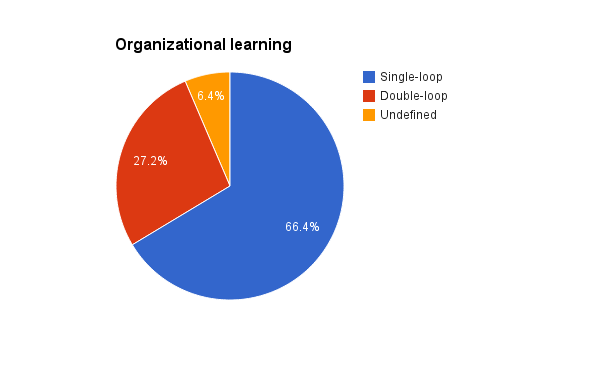
\includegraphics[width=\textwidth, keepaspectratio]{figures/learning-p.png}
	\caption{The distribution of single-loop, double-loop and undefined for all the actions.}
	\label{figure:learning-p}
\end{figure}

\begin{figure}[!h]
	\centering
	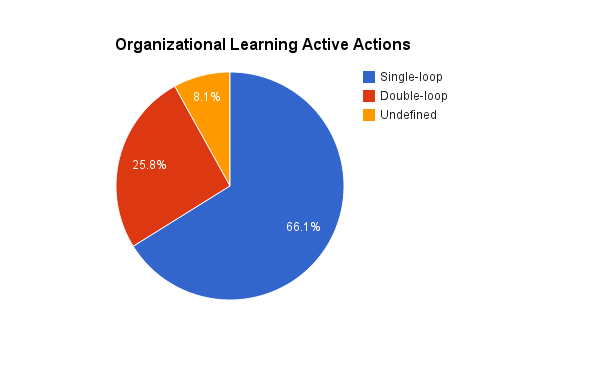
\includegraphics[width=\textwidth, keepaspectratio]{figures/learning-pa.png}
	\caption{The distribution of single-loop, double-loop and undefined for the active actions.}
	\label{figure:learning-pa}
\end{figure}

\begin{sidewaysfigure}[!h]
	\centering
	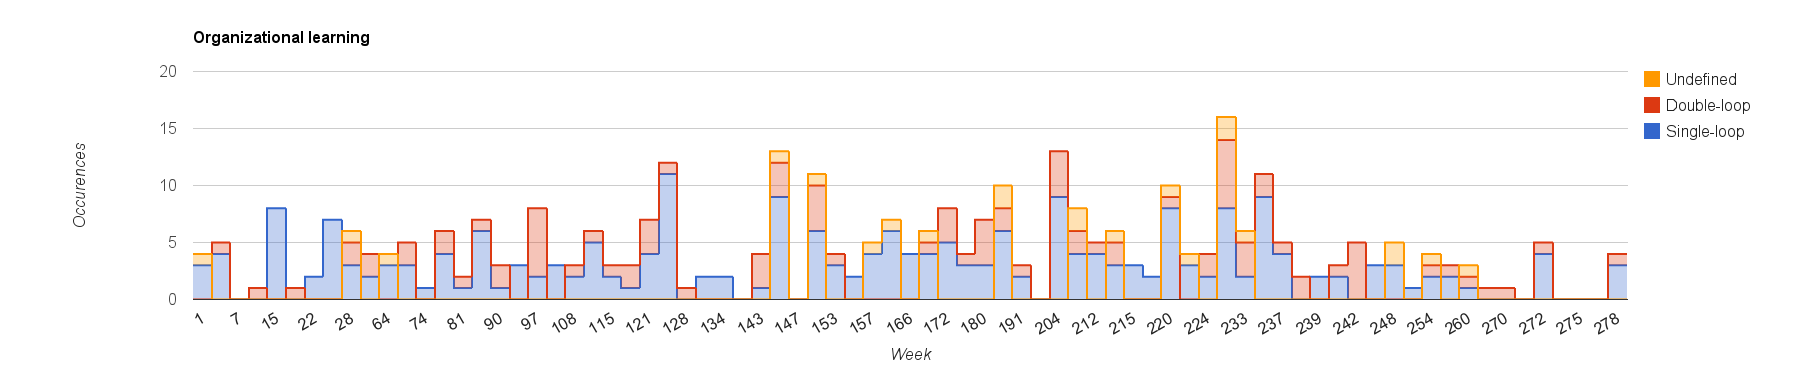
\includegraphics[width=\textwidth, keepaspectratio]{figures/learning-l.png}
	\caption{Timeline showing the distribution of learning loops for the total actions.}
	\label{figure:learning-l}
\end{sidewaysfigure}
\afterpage{\clearpage}

\subsubsection{Development Phase}
Planning, testing, development, and documentation were the four dominant phases in which an action were related according to our content analysis, as can be seen from \autoref{table:development-results} and \autoref{figure:development-p}. Planning being the biggest has a distribution value at 24.6\%. Second is the testing which 21.1\% of all the actions are related to. Development is related to 18.4\% and documentation is 13.2\%. Finally we have the remaining five categories Release, Build, Business Development, Bugfix and undefined which varies between 3.7-6.4 percent as can be seen in \autoref{table:development-results}. 
For the distribution of the different categories over time all of the categories are evenly distributed, in other words; No category is clustered to a specific period in time, but rather occurs evenly through the whole timespan. This can be seen in \autoref{figure:development-l}.
As have been the cases with the other themes the sub-group of the active actions mirrors the total actions with only minor variances as can be seen in \autoref{figure:development-pa} and \autoref{figure:development-p}.

\begin{table}[!h]
	\begin{center}
	\caption{Results from the content analysis in which development phase the action regards.}
	\label{table:development-results}
	\makebox[\textwidth]{%
		\begin{tabular}{| l | l | l | l | l |}
		\hline
		Category & \multicolumn{2}{|c|}{All Actions} & \multicolumn{2}{|c|}{Active Actions}  \\
		\cline{2-5}
		& Number & Percentage & Number & Percentage \\	
		\hline
		Development & 89 & 18.4\% & 11 & 13.1\% \\
		Testing & 102 & 21.1\% & 18 & 21.4\% \\
		Documentation & 64 & 13.2\% & 16 & 19\% \\
		Release & 18 & 3.7\% & 4 & 4.8\% \\
		Build & 23 & 4.8\% & 6 & 7.1\% \\
		Business Development & 18 & 3.7\% & 5 & 6\% \\
		Planning & 119 & 24.6\% & 19 & 22.6\% \\
		Bugfix & 20 & 4.1\% & 2 & 2.4\% \\
		Undefined & 31 & 6.4\% & 3 & 3.6\% \\
		\hline
		\end{tabular}
	}
	\end{center}
\end{table}

\begin{figure}[!h]
	\centering
	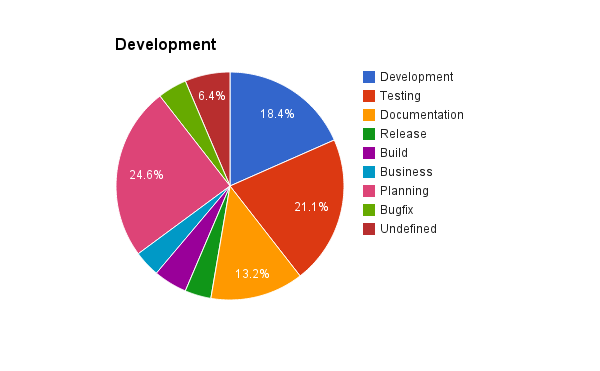
\includegraphics[width=\textwidth, keepaspectratio]{figures/development-p.png}
	\caption{The distribution of the different development phases for all the actions.}
	\label{figure:development-p}
\end{figure}

\begin{figure}[!h]
	\centering
	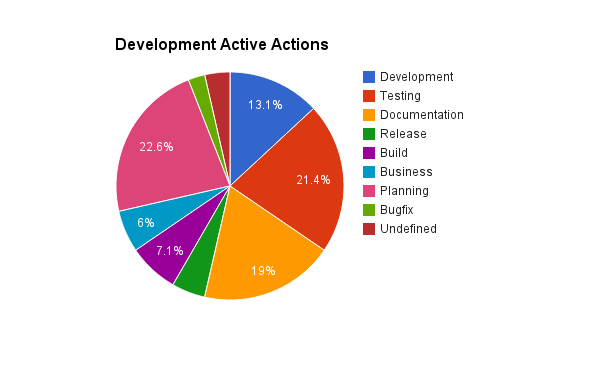
\includegraphics[width=\textwidth, keepaspectratio]{figures/development-pa.png}
	\caption{The distribution of the different development phases for the active actions.}
	\label{figure:development-pa}
\end{figure}

\begin{sidewaysfigure}[!h]
	\centering
	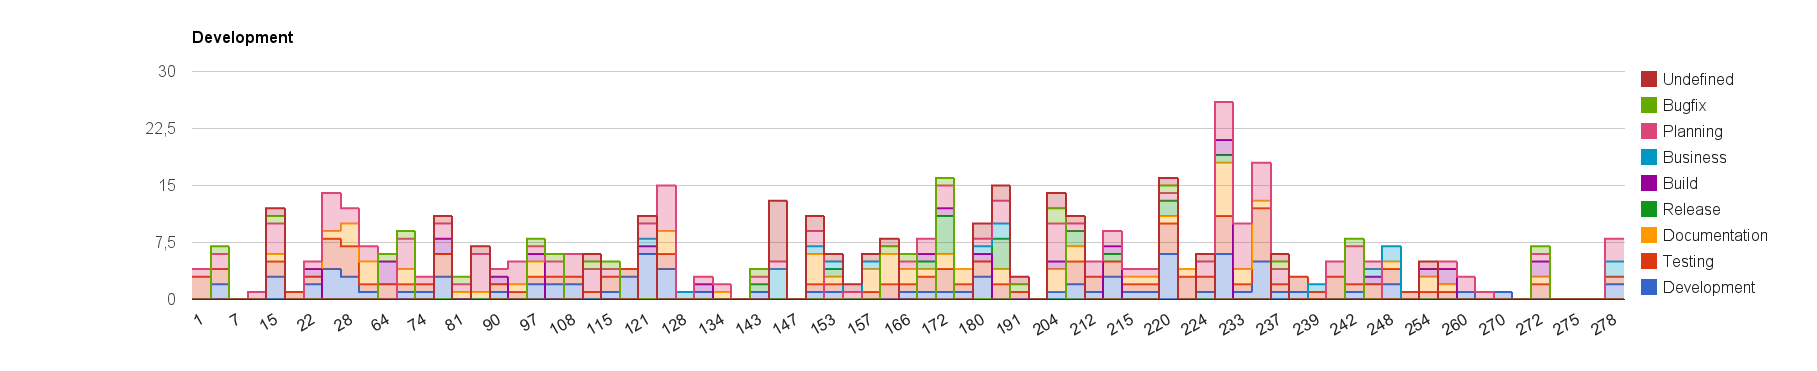
\includegraphics[width=\textwidth, keepaspectratio]{figures/development-l.png}
	\caption{Timeline showing the distribution of the different development phases over time.}
	\label{figure:development-l}
\end{sidewaysfigure}
\clearpage

\subsubsection{Collaboration}
Our results from the content analysis in terms of collaboration showed that 45.3\% of the actions were undefinable in terms of the analysis categorizations we had created. From the actions that were definable Communication was the biggest with 35.2\%. The second was external relations at 11.5\% and third competence at 6.9\%. Finally leadership was the smallest at 1.1\% of the total actions. The statistics can be seen in \autoref{table:collaboration-results} and \autoref{figure:management-p}. 
For the distribution of the different categories over time, \autoref{figure-management-l}, most of the categories was evenly spread across the whole timespan. the only exception to this is week 146 where there is a clear spike of external relations. This spike was a result of the team attending a network meeting in which they did a retrospective to better prepare them for the next network meeting. This anomaly will be disregarded further in the report. 
The active actions, \autoref{figure:management-pa}, shows that the three categories communication, competence and external relations evens out while leadership and undefined remains nearly the same only some small variances. However it is worth mentioning that the active actions are a sub-group of the total and thus this result is probably a skewed grouping. 

\begin{table}[!h]
	\begin{center}
	\caption{Results from the content analysis regarding the collaboration influences of an action.}
	\label{table:collaboration-results}
	\makebox[\textwidth]{%
		\begin{tabular}{| l | l | l | l | l |}
		\hline
		Category & \multicolumn{2}{|c|}{All Actions} & \multicolumn{2}{|c|}{Active Actions}  \\
		\cline{2-5}
		& Number & Percentage & Number & Percentage \\	
		\hline
		Communication & 128 & 35.2\% & 14 & 20.9\% \\
		Leadership & 4 & 1.1\% & 1 & 1.5\% \\
		Competence & 25 & 6.9\% & 1 & 11.9\% \\
		External relations & 42 & 11.5\% & 11 & 16.4\% \\
		Undefined & 185 & 45.3\% & 33 & 48.3\% \\
		\hline
		\end{tabular}
	}
	\end{center}
\end{table}

\begin{figure}[!h]
	\centering
	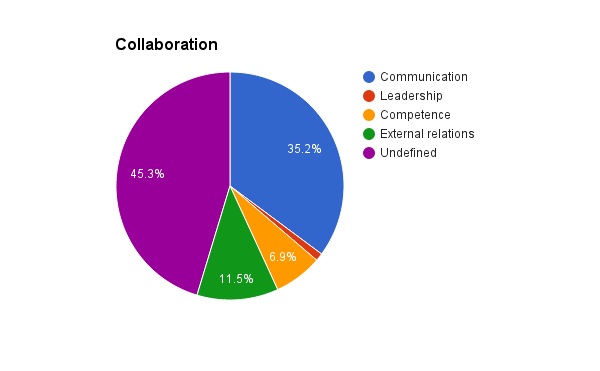
\includegraphics[width=\textwidth, keepaspectratio]{figures/management-p.png}
	\caption{The distribution of different collaboration categories for all the actions.}
	\label{figure:learning-p}
\end{figure}

\begin{figure}[!h]
	\centering
	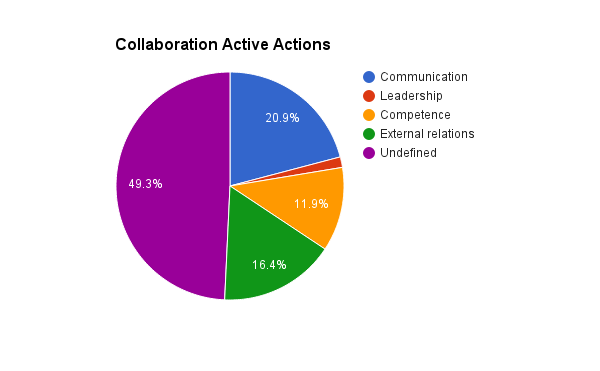
\includegraphics[width=\textwidth, keepaspectratio]{figures/management-pa.png}
	\caption{The distribution of different collaboration categories for the active actions.}
	\label{figure:learning-pa}
\end{figure}

\begin{sidewaysfigure}[!h]
	\centering
	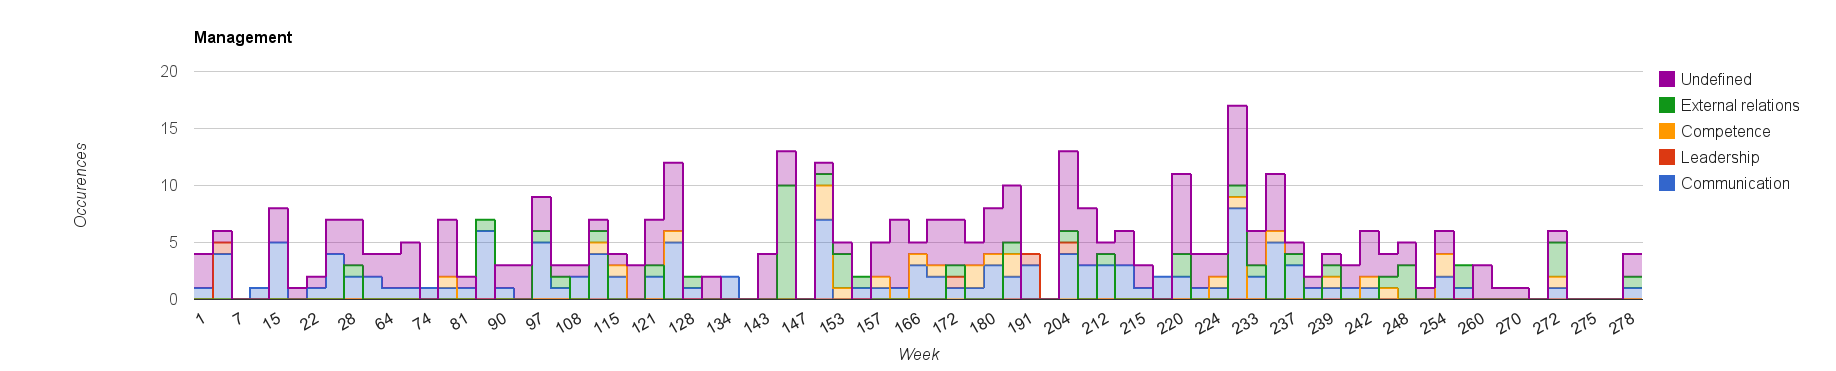
\includegraphics[width=\textwidth, keepaspectratio]{figures/management-l.png}
	\caption{Timeline showing the distribution of the different collaboration categories over time.}
	\label{figure:learning-l}
\end{sidewaysfigure}
\afterpage{\clearpage}

\subsection{Trends}
While conducting our content analysis of all the retrospective actions we uncovered some trends. By trend we mean actions that are related to the same issue/theme. We identified three trends being; Bugfix, Scenario Template and Developer-Tester Communication. We'll go through each of these in the following sub-sections. \todo{Write about comparing to active actions}

\subsubsection{Bugfix}
The first trend we recognized performing our content analysis was bugfixing. Developing computer systems is sure to create bugs and fixing them then becomes a natural part of developing software. In total we found 20 actions that was related to bugfixing. Of these two were purely technical actions, five were technical and process related and the remaining 13 action were purely process related. Of the 20 actions nine were related to communication between team members. In \autoref{figure:bugfix} one can see that the total amount of bugfixing actions has increased steadily throughout the timespan. 

\begin{figure}[!h]
	\centering
	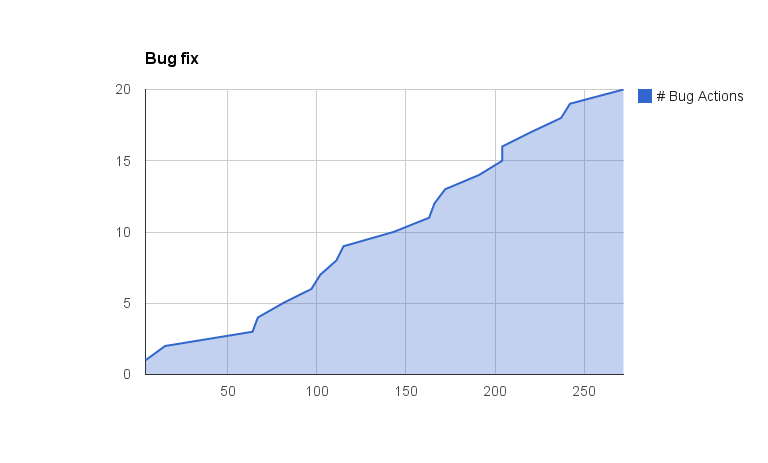
\includegraphics[width=\textwidth, keepaspectratio]{figures/bugfix.png}
	\caption{The total amount of bugfix actions over time.}
	\label{figure:bugfix}
\end{figure}

\subsubsection{Scenario Template}
For the second trend we discovered was in relation to a worktool called scenario template that team used to help specify requirements, create user stories and etc. In total we found 25 actions that were related to the scenario template. Of these 25 actions four of the actions were technical and process related, six were purely technical adjustments of the tool and 16 of the actions were process oriented on how the scenario template should be used. 18 of the actions were single-loop, only changing the effects which the scenario template provided. There were also six double-loop actions acknowledging root-cause issues with using the scenario-template and changes to reflect them. 
In \autoref{figure:scenario-template} the total amount of scenario template actions are shown over the 272 week long timespan. One can see that until week 163 the team has a slow increase in the number of scenario template actions. After week 163 however. a huge increase in number of scenario template actions occur. This continues until week 235, with a little slow period between week 180 and 205. At week 235 the team planned a meeting to go through the complete scenario template and after week 235 there are no more actions related to the scenario template. 

\begin{figure}[!h]
	\centering
	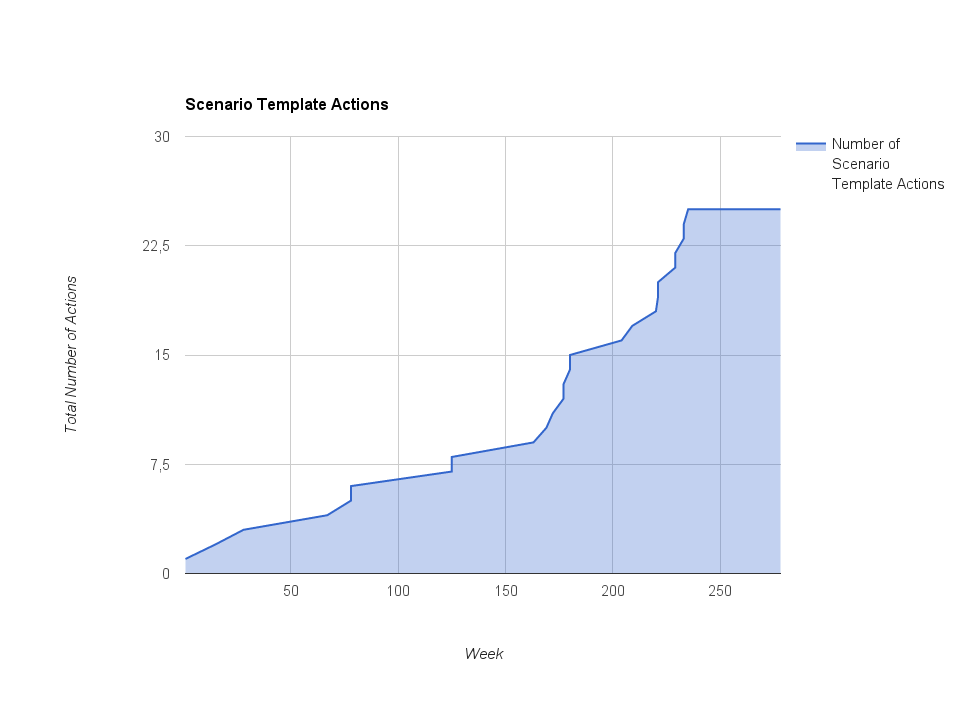
\includegraphics[width=\textwidth, keepaspectratio]{figures/Scenario-tpl.png}
	\caption{The total amount of scenario template actions over time.}
	\label{figure:scenario-template}
\end{figure}

\subsubsection{Developer-Tester Communication}
The final trend we observed during our content analysis was the communication between developers and testers. In total 25 actions were related to this. Of these 24 were process oriented and all the actions occurred from issues with a negative nature. 
\autoref{figure:dev-test-com} shows the distribution of the 25 actions over the 272 week long timespan. It can be seen that for the first 209 weeks that the amount of actions increase slowly with only two to seven actions every 50th week. After week 209 however we see a dramatic increase in the amount of actions, before it completely stops in week 238. We were not able to find any possible reasons for this sudden stop from reading through the reports. However as can be seen from \autoref{figure:dev-test-com} there has been periods between actions as long as 45 weeks so it is possible that this stop can be such a break.  

\begin{figure}[!h]
	\centering
	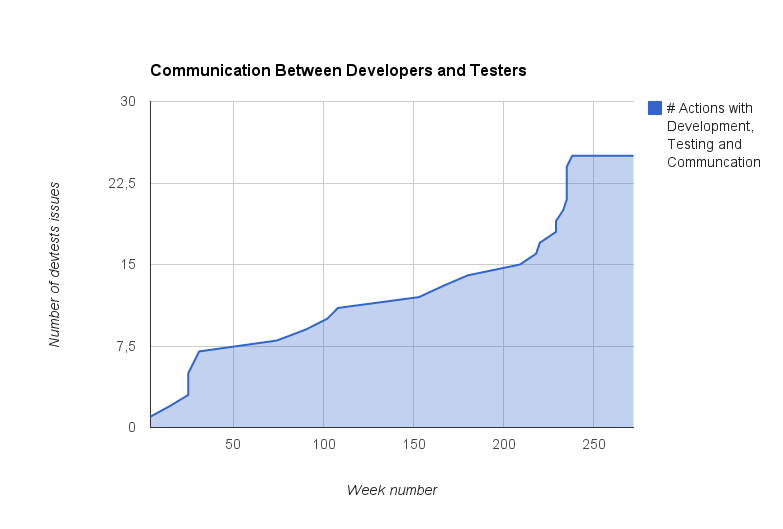
\includegraphics[width=\textwidth, keepaspectratio]{figures/devtestcom.png}
	\caption{The total amount of developer-tester communication related actions shown over time.}
	\label{figure:dev-test-com}
\end{figure}

\clearpage

\section{Feedback Session}
After performing our content analysis, we visited the team to present our analysis results as well as receive feedback from the team. In this section and its following sub-sections we'll present the results from this session. We will start with going through the feedback on the key numbers, before we continue on the categories and trends and finally take anything else that came up during the session. 

\subsection{Feedback: Key-Numbers}
When presenting the key-numbers the team mostly found our results agreeable with their own thoughts. The only surprise to the team was the amount of active actions. Their surprise came as they believed the number of active actions to be higher. The reason for this belief was that they thought they were worse at closing actions as the list of active actions seemed so long, but compared to the amount of total actions it seemed more reasonable. However it was pointed out that existing actions hinder new actions for the same problem to be created and thus the amount of active actions might not be accurate with how the team works with the problems as a actions might not be documented, but worked on never the less. 

When raised the question why the decrease of actions after week 237 the team gave their thoughts. During the period the decrease in number of actions they had acquired a new foreign developer within the team. Unfortunately the new developer had not lived up to the task creating what the team called an ``Elephant in the room''. The situation absorbed the other problems within the team as no one would be rude and tell that the new developer that he were the problem. As one of the team members described during the feedback session: 
\begin{quote}
``We actually discussed it once at the coffee after lunch, the retrospectives at the moment were just a waste of time''. 
\end{quote}
When asked what was the reason for the developer not living up to his expectations the team told us that face-saving and cultural differences made it difficult to communicate properly and that tasks that were assigned to him weren't satisfiable. 

The developer quit the team after a period of 34 weeks in week 263. This still means that the low action period of 15 weeks between and week 263 and 278 remained unexplained. When inquired about this the team had several possible reasons. One were that there were already to many active actions on the plate resulting in fewer getting made. Another were that the communication within the team improved after team had lost the developer creating the problems. A final possible reason was that the secretary for the retrospectives changed a lot within that period of time. 

After discussing the decrease in actions period the team mentioned that it would be interesting to see if there were any correlations between retrospective actions and team changes other than the one already explained. We have in the time after the visit to the team created such charts as can be seen in \autoref{figure:team-changes} and \autoref{figure:secretary-changes}. 

In \autoref{figure:team-changes} we can see that the period of low actions starting at week 237 and lasting out week 278. In that period the foreign developer, T7, joins and leaves the team. In the same period the SCRUM master of the team takes a leave of absence for a period of 20 weeks which also might have influenced the period. 

For the secretary changes, shown in \autoref{figure:secretary-changes} we can see that the changes in who writes the reports doesn't seem to influence the number of actions that comes out of the actions. The only exception to this could be the period after week 263 where there are a lot of changes, as the team described. However we believe this to be unlikely as between week 270 and 275 the secretary stays the same and the amount of actions follows the trend of low number of actions and as changes earlier in the timespan haven't revealed any effects. 

\begin{sidewaysfigure}[!h]
	\centering
	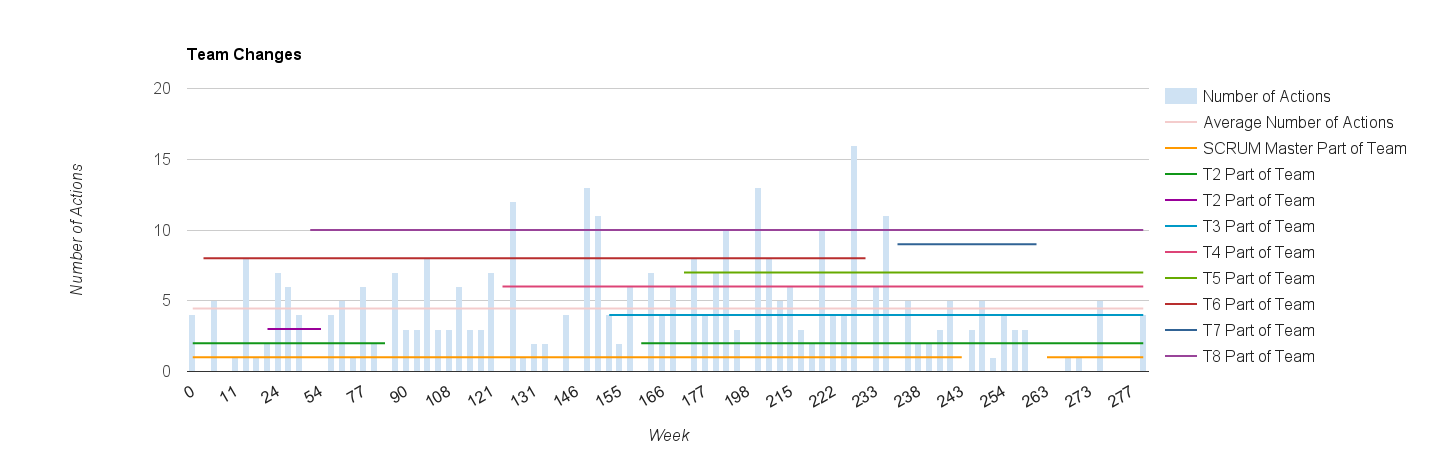
\includegraphics[width=\textwidth, keepaspectratio]{figures/team-changes.png}
	\caption{Team changes and the amount of actions for the retrospectives across the 278 Weeks.}
	\label{figure:team-changes}
\end{sidewaysfigure}

\begin{sidewaysfigure}[!h]
	\centering
	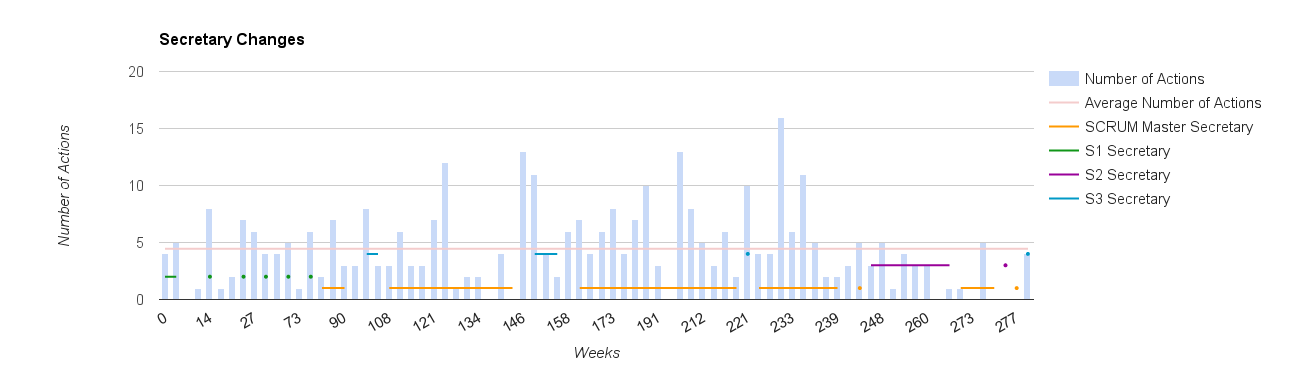
\includegraphics[width=\textwidth, keepaspectratio]{figures/secretary-changes.png}
	\caption{Secretary changes and the amount of actions for the retrospectives across the 278 Weeks.}
	\label{figure:secretary-changes}
\end{sidewaysfigure}
\afterpage{\clearpage}

\subsection{Feedback: Categories and Trends}
In this section we will present the thoughts of the team as well as their reactions on the results of the content analysis. We will start with the nature of the actions and then continue on context, decision making, organizational learning and development phase and finally we will go through the collaboration categories and trends. 

\subsubsection{Nature}
The results from the nature context did not surprise the team at all. We asked if they would like the guess what the ratio between positive negative would be and they said one-to-nine, which is quite close. Our results revealed five percent undefined and five percent positive with the remaining 90 percent negative. The team described themselves as problem-oriented and reasoned that this is the cause for the high amount of negative actions. They also said that they do during the retrospectives talk about good things that has happened, but as they are problem oriented it rarely gets documented. 

\subsubsection{Context}
Our results from the content analysis revealed that 58 percent came from a process context, while 40 percent came from a technical context. When this was presented to the team they thought it would be more technical than process actions. The reason for this wasn't elaborated during the session. It was however elaborated on the results of the active actions which the analysis revealed had a little more technical actions than process ones. The team said this was not so surprising as some of the technical actions could require a lot of time to complete. 

\subsubsection{Decision Making}
The team thought that it was a good sign that the team were able to do strategic decision making. When we presented the results for the decision making analysis, the team was pleased to see that they had all of the three categories represented. They were especially pleased to see that the there was a substantial portion of strategic actions. We asked what could be the reason for this and the team responded that they felt autonomous. As they described the company allowed the different development teams to have a fairly large independence allowing room to do strategic choices within the team. 

\subsubsection{Organizational learning}
When we presented the team to our results in terms of organizational learning the assumptions they had was as expected. They use the term of direct causes as single-loop and root causes as double-loop, but we will continue using the terms of single-loop and double-loop. They expected that single-loop would have the most occurrences, even though they maintained a double-loop focus during the retrospectives. This expectation is reflects our results quite well as 66 percent were single-loop and 25 percent double-loop. The reason they expected it to be more single-loop rather than double-loop was that it was easier to do single-loop and as one team member said: ``...sometimes things just need to be fixed''. 

\subsubsection{Development Phase}
The results from the content analysis were quite different from the team expectation in the context of which development phase the actions were related. The team expected that build and documentation would be the two biggest actions. The content analysis revealed that planning was the biggest followed by testing, development and documentation. The team thought this made sense as most of the planning is directed towards process improvement and they do focus on process during the retrospective. The team speculated if the releases might have a correlations with planning actions coming right after. \todo{Correlation release planning and release actions}. It was also again mentioned that actions might not be created even though they were discussed as actions already existed and that they had not been completed. 

The team expected build to be the phase that occurred most. It was a surprise that it was not better represented within the actions as it felt that it was discussed often on retrospectives. One of the members said that the lack of actions specific for builds might be the reason while it was discussed during retrospectives and that they might focus on creating more actions related to the builds. 

We asked the team if there were any categories they missed from the development phase analysis and two were mentioned. The first one was hotfix which the team often mentioned during the feedback session. The second one was flow as to how the development of the product progressed. For future similar analyses this should be taken into considerations. 

\subsubsection{Collaboration}
For the collaboration the team expected communication to be the category with the most actions. If you disregard the undefined actions which was the biggest in terms of collaboration the teams expectation was correct. We asked if they could explain what kind of communication that were discussed most during the retrospectives. They said that communication between the different stages of the development and more oral communication rather than written was the kinds of communications that were discussed the most. As for the other categories the team had no special feedback. 
\chapter{Discussion}
Our goal for conducting these studies were the following: \textit{Our goal for this study is to investigate the outcome returned from the retrospective in terms of organizational learning and retrospective characteristics.} Throughout this chapter we will first provide a descriptive discussion on the retrospective characteristics we have observed and then discuss the results in terms of organizational learning. Finally we will provide some reflections on the retrospective practice, the current state, a method proposal and some guidelines for conducting retrospectives. 

\section{Retrospective Characteristics}
One of our research objectives were: \textit{What are the main characteristics in current retrospective practices, in
terms of outcome, processes and impediments?} Throughout this section we will provide a descriptive discussion on the characteristics we have identified throughout our studies. The section is split into three parts: Output, Process Characteristics and Impediments. An overview of all the characteristics can be seen in \autoref{table:retrospective-properties}

\begin{table}[h]
	\begin{center}
		\caption{Retrospective characteristics}
		\label{table:retrospective-properties}
		\begin{tabular}{p{0.9\textwidth}}
			\hline
			\textit{Retrospective Characteristics}\\
			\hline
			\textbf{Output} \\
			Reflection on work processes, technical issues, work environment \\
			Creates improvement opportunities \\
			Improvement Implementation \\
			Provides organizational learning \\
			Improves shared mental model\\
			Can improve team enthusiasm \\
			Can decrease team enthusiasm \\ 
			Can improve efficiency  \\
			Facilitates empowerment \\
			\hline 
			\textbf{Process Characteristics}\\
			Little Considerations Taken \\
			Wish to Improve \\
			Varying techniques\\
			Occurs regularly\\
			Collects opinions from participants\\
			Arena for open discussion \\
			Allows for experiments in work environment\\
			Shared Learning Event\\
			\hline
			\textbf{Impediments}\\
			Team commitment\\
			Enforcing of process improvement actions\\
			\hline
		\end{tabular}
	\end{center}
\end{table}

\subsection{Output}
In this section we discuss the observations regarding the output of a retrospective process. The section is divided into ``Work areas'', ``improvements'' and ``Enthusiasm''. Some of these sections are divided into subsections, where we discuss relevant observations.

\subsubsection{Work areas}

Several work areas are covered by the retrospective. Mainly we have seen three areas that are covered by the retrospective. These areas are work processes, technical issues and issues related to the work environments. As we saw in team Zulu about 40\% of the actions created were related to technical issues and 59\% to process issues. Some of these issues might have been work environment related, however our content analysis did not include this. For future work this should be considered. From the interview with team Echo we learned that the team mostly discussed work environment issues as the team consisted of several sub-teams that worked differently from each other. 

We have seen very little of personnel issues brought up during the retrospective. Only case was with team Delta where one of the members never got help from the others. In team Zulu we saw that not being able to take up personnel issues hindered the retrospective. When asked several of the study participants voiced an opinion that personnel issues were something that should be taken outside of the retrospective to hinder blaming and a negative mood during the meeting. We have not seen any earlier literature discussing the topic. We do believe however that the consideration of including personnel issues is something that could be appended to Dingsøyr's \cite{Dingsoyr2004} set of considerations which should occur before the retrospective.

\subsubsection{Improvements}
Here we discuss the improvement outputs from a retrospective process. The outputs discussed are ``Creates Improvement Opportunities'', ``Improvement Implementation`'', ``Improves Shared Mental Model'' and ``Shared mental models practice`''. 

\paragraph{Creates Improvement Opportunities}
Through our studies we have seen that teams are able to improve based on decisions created during the retrospective. From the depth study of Team Zulu's we saw that through 77 retrospectives the team had created 343 actions which reflects improvement opportunities. Also all the teams in our breadth study created actions to improve some aspect of their work-life. It is clearly evidence that improvement opportunities are created through the retrospective. This seems to fit well with previous \cite{Larsen2006, Dingsoyr2004, Drury2012} that the retrospective help identify improvement opportunities. 

\paragraph{Improvement Implementation}
The question if the improvement opportunities are actually implemented can also be seen through our studies. The results of our studies revealed that most of the teams were satisfied with their implementation rate. From team Zulu we learned that only 65 of the 343 actions were not yet implemented. It was also revealed that implementation could be a challenge, as was the case with Team Charlie. We identified two methods that seemed to help overcome this challenge. The first was assigning responsible team members to each action. The second was SCRUM master follow-up of the actions. We have seen that retrospective practicing agile development teams are able to implement improvement opportunities confirming Derby and Larsen's \cite{Larsen2006} statement of retrospective helping team adapt and contradicting the research of Drury et. al. \cite{Drury2012} which finds that no real changes occur as a result of the retrospective. 

\paragraph{Improves Shared Mental Model}
The knowing stage is not included in the domain of the sprint retrospective described by Petter et al. \cite{Petter2013}, in our work we found that the facet of team members sharing their individual knowledge, thereby updating the shared information. One example of this was found in team Echo, where the different sub teams would use the retrospective to share their discoveries and knowledge development, thus updating the meta-knowledge of the team as a whole. 

The learning phase of the shared mental model and is impacted by the agile retrospective by using techniques that facilitate the integration of the knowledge from the knowing stage. One example could be the use of evidence based time lines as described by Bjarnasson et al. \cite{Bjarnason2012}, where the time line would work as an outline of the information received by the team. Another example is seen in the weekly retrospectives held by team Alfa, where team members would continually update their colleagues on their work day, allowing for reflexivity. Another example would be the use of the ``five times why'' as used by team Charlie and Echo, where both the possibility for reflexivity and self correction exists.

The understanding phase described by Petter et al. \cite{Petter2013} is far reaching and includes many facets of team cooperation and some of them are described in \autoref{section:mental-models-stages}. One part of the understanding phase we did not expect to see explicitly in our study was conflict resolution on a personnel level, and can be considered part of the conflict reconciliation and consensus building that is part of the understanding phase. Also part of the understanding phase is the practice of refining team communication and team processes which is a central component of the retrospective purpose, and we observed every team discussing these topic during our interviews and analysis. Lastly, not included in the work of Petter et al. is the use of the retrospective as a tool for planing, and 24.6 percent of the actions analyzed in our work with team Zulu were deemed to have a planning component, as described in \autoref{section:development-phase}. This planning component could be said to be increasing the similarity of the information between team members.

The execution is perhaps the phase most impacted by the retrospective, as the explicit actions decided during a retrospective almost always is intended to improve or refine the processes that in one way or another help the reach their goals. For example the information similarity generated in the understanding phase can lead to a quicker response time to new tasks. One typical example is the refining of the communication processes as seen in team Zulu, or the introduction of the bug-fix days described in \autoref{section:bugfix}. 

\paragraph{Shared mental models practice}
In this section we discuss observations on the relationship between retrospectives and shared mental model practices.

Reflectivity is a central part of the learning process in the team. We have observed that many teams use the retrospective as a review tool of the last work period. We have observer very different practices when it comes to frequency as seen in \autoref{table:frequency-duration}, and thus the definition of a work period is different from the sprint retrospective definition from Peter et al. One observation done by us is that very few teams practice reflectivity on the retrospective itself, or if they do they do not formally do it on the team level, as seen in team Charlie. In team Charlie the scrum master would discuss and reflect on the retrospective with other scrum masters and team leaders within the company, but it would not be brought back to the team. In some ways the analysis done with team Zulu together with the feedback sessions with them could potentially be considered an example of this kind of reflectivity. The interviews done with team Zulu's leader and scrum master suggests that both the team's mental model similarity and accuracy was improved through the analysis and reflection done, this is described in \autoref{section:feedback-session 4}

The sprint retrospective defined by Petter et al. Does not include planning, but our work with team Zulu indicates that planning is an integral part of retrospective actions in some teams. This is discussed in \autoref{section:development-phase}, this high degree of presence of planning was unexpected and more thought on the potential of mental model improvement through planning in retrospective seems interesting. For example the use consensus based approach used by team Golf in planning could potentially increase the similarity of the team's mental model.

\paragraph{Can Improve Efficiency}
The retrospective practice can, as we have seen in multiple examples, improve the efficiency of teams conducting them. Team Echo's practice changes from SCRUM to KANBAN and then to modified SCRUM and Team Zulu's ``Bug-crunch day'' is just two of the examples we have seen that the teams have been able to improve their efficiency through the retrospective practice. This again confirms the previous literature \cite{Dingsoyr2004, Larsen2006, Kinoshita2008} that retrospective are able to improve practices and contradicts the finding of Drury et. al. \cite{Drury2012} that retrospectives provides no real changes.

\subsubsection{Enthusiasm}
\label{section:positive-loop-enthusiasm}
Team enthusiasm is both affected the retrospective practice and inflicted by it. It can be increased through a positive feedback loop or decreased by a negative feedback loop. As a result of the retrospective practice individual empowerment is facilitated and this also increases the enthusiasm. We will describe and discuss each of these statements below through examples from our studies and earlier literature. 

\paragraph{Can Improve Team Enthusiasm}
We seen that the enthusiasm of the participants of retrospective practice can be both affected by the retrospective. We uncovered a positive loop that helps increase the enthusiasm of the team conducting retrospectives. If changes occurred as a result of the retrospective the participants would become enthusiastic and thus the chance of more changes would occur. Ownership towards the development process was one factor that could help increase the enthusiasm and feed the positive loop. The positive loop confirms what Derby and Larsen \cite{Larsen2006} states that teams are invested in the success of improving their work as the improvements are chosen by the teams themselves and not from upper management. 

\paragraph{Can Decrease Team Enthusiasm}
The retrospective practice has also the ability to decrease the enthusiasm of the practicing team. As the opposite of the positive loop a negative are able to decrease the enthusiasm. If no changes occur enthusiasm will decrease and as the enthusiasm decreases the chance of new changes occurring decreases. Some even might see the retrospective as a waste of time as described by team Charlie's SCRUM master which had happened with some of the teams in his department. This confirms our previous literature review \cite{Dolvik2014} that recurring issues kills the joy and Drury et. al. \cite{Drury2012} that some may see the retrospective as a waste of time. 

\paragraph{Facilitates Empowerment}
Ownership towards the development process was seen as crucial towards getting improvement out of the retrospective by the interviewed teams. Each team member has the possibility to participate in shaping their working process through the retrospective. As seen in team Alfa and Echo even the shy are required to participate in returning feedback and contribute solutions for current work processes. Tessem \cite{Tessem2014} identifies participation in process improvements as an empowering practice. This directly relates to the retrospective practice, which is also a parallel drawn by Tessem and we now confirm. Enthusiasm is increased as members are empowered\cite{Tessem2014} and thus the retrospective increase enthusiasm through empowerment. 

\subsection{Processes Characteristics}
In this subsection we will discuss the process characteristics observations we made in relation to our results and established theory. The subsection will be divided into before, during and after.

\subsubsection{Before}
As seen in \autoref{section:Dingsoyr-Approach-Introduction} we will compare our observation results of the work done before a retrospective primarily to the theory from Dingsøyr's ~\cite{Dingsoyr2004} work. This section is divided into ``Little Considerations Taken'', ``Wish to Improve'' and ``Facilitator''.

\paragraph{Little Considerations Taken}
When we consider our results we see that few of the teams interviewed do a thorough consideration of their practices in relation to the approaches seen in \autoref{table:postmortem-approach}. Most teams did not do a informed decision on several Dingsøyr's considerations. For example on who to invite or sharing tacit and explicit knowledge. For example team Alpha's interviewee said that it could go long periods of time where a developer was not invited to a retrospective. When it comes to sharing the knowledge generated none of the teams made a concerted to share the knowledge that came as a results of learning through the retrospective.

\paragraph{Wish to Improve}
Many teams had a great wish to improve. As seen throughout our results the need to build a culture that allows for learning is absolutely essential for a productive environment, this is in accord with  Dingsøyr's work. Especially trust between the team members emerged as critical for reaching the maximum potential of a retrospective session. An example of the possible improvements is the team dynamic improvements experienced by team Delta when one of their team members brought up the problem that he was not getting help from other team members, as described in \autoref{question-21}. Also after our depth analysis with team Zulu their eagerness to improve let them turn the results from our analysis into a basis for multiple actions intended to improve the team's learning capabilities. 

\paragraph{Facilitator}
\label{section:facilitator}
Deciding on the facilitator can be considered both part of before the retrospective, and during. As work needs to be done in advance and Few teams used an external facilitator as recommended and the experiences we observed were uniformly positive. This is in accord with Dingsøyr's work. However only two teams used external facilitators consistently, as described in \autoref{question-12}. Team Zulu had only one experience with using an external facilitator but it was described as a very productive and positive experience. Perhaps this indicates that many teams would benefit from making a more concerted effort to utilize external facilitators. 


\subsubsection{During}
In this section we will discuss our observations relating to what happens during the retrospective process. This is divided into ``Occurs Regularly'', ``Collects Opinions from Participants'' and ``Open Arena for Discussion''.

\paragraph{Occurs Regularly}
Retrospectives happens at a regular basis varying from team to team from every week to every six months. Usually it occurs after an ending of a development stage either a project iteration or a released feature.

\paragraph{Collects Opinions from Participants}
During the retrospective data is gathered from the participants. We have seen that feelings and opinions are two primary data types gathered. None of the teams in this study have used other sources of data for their retrospective, with one exception of lead times which were used by one of the teams. The participants in the retrospective consists of team members contributing to a project iteration or feature that the retrospective focuses on. These consists of developers, testers, designers, architects,consultants, SCRUM masters and in some cases project leaders as seen in Team Zulu. 

\paragraph{Open Arena for Discussion}
The retrospective provides an open arena for discussion. Each participant are allowed to bring their own issues and the issues are then analyzed through discussion or root-cause analysis. An facilitator, either internal from team or external, facilitates the discussion. From the facilitators we have spoken to some censor the discussion on some subjects. In team Alfa personnel cases where not allowed and would have to be discussed outside the retrospective. In team Delta the SCRUM master tried to hinder technical discussions as their focus is on work processes. Other than this most topics are allowed during the retrospective as we have seen in Team Zulu. Through our depth study we saw that.

\subsubsection{After}
In this section is our discussion on factors that take place after the retrospective process. This is divided into ``Allows for Experiments in the Work Place'' and ``Shared Learning Event''. 

\paragraph{Allows for Experiments in the Work Place}
\label{section:experiments-in-work-place}
As seen in \autoref{section:Derby-Larsen-Structure} a retrospective can be an area that facilitates experimentation in a team. We have observed this, for example as described with team Echo in section \autoref{question-11}. Here team Echo tried to move to KANBAN from SCRUM, the experiment was not an immediate success, but allowed them to return to a SCRUM methodology that they could tailor after their experiences from the experiment. This resulted in their work methodology fitting their team better. Our work with team Zulu also led to experimentation, for example their decision to create a dashboard to log their retrospective actions. Another experiment by team Zulu was the inclusion of a ``bug-crunch'' day seen in \autoref{question-11}. This experiment was a success and led to a noticeable decrease in bugs.

\paragraph{Shared Learning Event}
The theory of the retrospective as a shared learning event was described in \autoref{intro:retro-outcome}.  An example of a shared learning event from the same section was performed by team Delta, as they changed their time estimation practices to great success after discussing the process in a retrospective. However none of the teams interviewed made an organized effort to make the result of the retrospective a learning event for personnel outside the team, as mentioned by Dingsøyr ~\cite{Dingsoyr2004}.



\subsection{Impediments}
In this section we discuss our observations on impediments in context of the retrospective process. The sections is divided into ``Personalities'', ``Team Commitment'', ``Enforcing of Process Improvement Actions'' and ``Availability''.

\paragraph{Personalities}
Some personalities could provide obstacles for the retrospective. We saw three examples of this. The first one was in Team Zulu where cultural differences provided miscommunication and difficulty providing an open discussion in the retrospective. The second was in the department to team Charlie where some SCRUM masters had low enthusiasm for the retrospective practice and this could influence the rest of the teams as well. The third example were two senior developers with strong personalities, in team Charlie, that could hinder the other developers from voicing their opinions. These were the only three cases we saw in our studies, but further personalities may be investigated. Derby and Larsen \cite{Larsen2006} talks about personalities that take a lot of time and hinder others from taking part in the retrospective and this is reflected pretty well in the last example. They suggest that talking to them privately and directly asking them to hold back a little could help the situation. Team Alfa recommended using KJ-sessions to help everyone participate.

\paragraph{Team Commitment}
Even though most of the teams in our study was satisfied with the commitment from their teams, implementation of actions still could provide a challenge. As mentioned by several of the interviewees if the actions were not assigned to a specific person the action would not be implemented. This indicates that the team as a whole don't have the commitment to implementation of retrospective actions. Drury et. al. \cite{Drury2012} described several obstacles that it fits with these results. Team members unwilling to commit and relying on SCRUM master, not implementing decisions or relying on others for decisions, and not taking ownership of decisions are all obstacles that could be identified through our research. However as mentioned this was only the case when the group as whole was assigned to a decision, when individuals of the group were assigned the teams were satisfied with the implementation rate. This still indicates however a lack of team commitment even though the consequences are dealt with. 

\paragraph{Enforcing of Process Improvement Actions}
Enforcing the implementation of process improvement actions were seen as a challenge. The SCRUM master of team Zulu described how enforcing and monitoring process improvement actions was a challenge. Some process changes required the whole team to implement the action and both enforcing the implementation and monitor it could be hard. Conflicting priorities and not taking ownership for decisions are two of Drury's et. al. \cite{Drury2012} obstacles to effective decision making, and these results reflects the two obstacles. 

\paragraph{Availability}
The last impediment we have seen for conducting retrospective is availability. In team Golf we saw how having a distributed team could make it harder to conduct the retrospective. In team Alfa and Foxtrot we learned how the unavailability of retrospective due to long timespan or participants not being able to participate could inhibit the retrospective. Zedtwitz's \cite{Zedtwitz2002} barrier of memory bias and Drury et. al. \cite{Drury2012} obstacle of unavailable staff is reflected in this. 

\clearpage

\section{Organizational Learning} % (fold)
One of our research objectives were: \textit{How is learning achieved through current retrospective practices, in light of organizational learning theory?} Throughout this section we will first discuss the results of our case-studies in terms of the governing values of Argyris and Schön's \cite{Argyris1996} organizational learning Model I and Model II. Secondly we will discuss our results in terms of learning types. Finally we will discuss the impediments for learning that we have seen throughout our studies. 

\label{sec:organizational_learning}
\subsection{Governing Values}
Argyris and Schön\cite{Argyris1996} described several governing values for learning organizations as we described in \autoref{intro:organizational-learning}. Throughout this section we will reflect on our results using these governing values investigating how retrospectives is performing as a learning practice. 

\subsubsection{Model I}
In Model I, described in \autoref{sub:model_i}, four governing values set the focus for the learning organization. Into our investigation of the retrospective practice we have seen very little to any of these values. We will discuss this below for each governing value and then the consequences before we summaries the findings related to Model I.  

\paragraph{Setting and  Achieving Goals}
One could argue that the team setting goals and achieving them could be compared to creating actions and fulfilling them, however we do not support this as the fulfillment of actions is part of a collective efficiency improvement and learning practice. The retrospective and its participants are instead of trying to design and manage the environment unilaterally, investigating all the different angles and perspective the team can present and finding solutions to the problems existing within that environment. The joint team discussion and retrospective practices are evidence of this. 

\paragraph{Maximize Winning and Minimize Losing}
Maximizing winning and minimizing loosing is not visual in the current retrospective practice. The teams are not afraid to use the retrospective as an arena for creating experiments on new practices where some might work and some might not. Team Delta and Echo, gave examples where the teams had tried to implement new practices and instead of going down with ship when the practice had not worked, leave ship and try something else. In Team Delta things that did not work for the members of the team simply did not get done and it was a joint understanding that actions that did not get any attention were bad practices. In Team Echo the team was not satisfied with current work practices and changed them drastically. After some months time they found that these new practices only made thing worse and instead of claiming ownership for the task and try to force it through the team decided to try something new. 

\paragraph{Minimize Generating or Expressing Negative Feelings}
Through retrospectives we have seen that the participants are allowed to express their feelings regardless of their good or bad. This effectively counter the third governing value which is minimizing generating or expressing negative feelings. Team Echo and Delta both described events that showed participants raising negative issues and feelings towards the team. From the retrospective analysis for Team Zulu we saw that 89.3\% of the actions created came from negative issues. Even though allowing negative feelings are good thing some of the interview subjects said it could become a little bit to much negative sometimes, and that the retrospective is not a arena to vent. As was the case with Team Zulu the third and fourth feedback session revealed that the team had become more aware of raising also good feelings and issues during the retrospective and such they felt the retrospective had improved. This indicates that allowing negative feelings is important as one can learn and improve from them. However one should also ensure that good feelings are raised as they also provides the same opportunities and creates a more enthusiastic feeling about the retrospective.

\paragraph{Be Rational}
As feelings are encouraged to share during the retrospective, to some moderation, the fourth governing value being rational also seemed to not be the apparent in the retrospective. Being rational implies censoring feelings and as we described above retrospectives encourages sharing of feelings towards the group. 

\paragraph{Consequences}
The consequences resulting from Model I governing values also seems to be rarely encountered in retrospectives in terms of the behavior. We have witnessed one case where an actor acted defensibly and such created an atmosphere that suppressed the other participants feelings. Creating what was described in an elephant in the room. It was also confirmed by the interviews that personnel issues were not addressed during the retrospective and such events could decrease the value gained from the retrospective. Other than this we have neither seen or heard about teams having defensive norms, or having defensive interpersonal relationships. 

Most of the learning consequences seems to be opposite of what is expected by Model I except single-loop learning and possibly decreased long-term effectiveness. It might not be that surprising that as the governing values are rarely encountered that the consequences of them is not either. Neither self-sealing, lack of public testing of theory or too much testing of theory in private seems to be appearing in teams conducting retrospectives. What is more surprising is that single-loop is quite occurring. We will dwell deeper into this in \autoref{discussion:learning-types}. In terms of decreased effectiveness we have no way compare these to any of our results as we lack a control group applying most of the governing values from Model I. 

\paragraph{Model I Summary}
The governing values from Argyris and Schön's Model I seems to not occur or be the system employed by agile development teams performing retrospective systems today. We have only seen two cases where the governing values of Model I has had any implications on the team. The first one was that of face-saving from one of the team members resulting in an atmosphere suppressing the other members feelings. This member later left the team. The other implications of Model I governing values is that of single-loop learning which most teams experience and will be discussed further in \autoref{discussion:learning-types}

\begin{table}[h]
	\begin{center}
		\caption{Governing values and consequences encountered in relation to retrospectives.}
		\label{table:model-i-occurences}
		\begin{tabular}{l l}
			\hline
			\textit{Model I} & \textit{Encountered} \\
			\hline
			\textbf{Governing Values} & \\
			Defined goals and try to achieve them. & No \\
			Maximize winning and minimize loosing. & No \\
			Minimize generating or expressing negative feelings & No \\
			Be rational & No \\
			\hline
			\textbf{Behavioral World Consequences} & \\
			Defensive Actors & Once observed \\
			Defensive Interpersonal and group relationship & No \\
			Defensive Norms & No \\
			\hline
			\textbf{Learning Consequences} & \\
			Self-sealing & No \\
			Decreased long-term effectiveness & Not observed \\
			Single-loop learning & Yes \\
			Little testing of theories publicly & No \\
			Much testing of theories privately & No \\
			\hline
		\end{tabular}
	\end{center}
\end{table}

\subsubsection{Model II}
The governing values of Argyris and Schön's Model II are more apparent in the teams that practice retrospectives. We will discuss our findings related to each of the governing values and the consequences observed below. A summary of this discussion is at the end of the subsection. 

\paragraph{Valid Information}
Valid information is the first of the governing values of Model II and the retrospective practice require information gathering from the team members. We have seen several ways that retrospective teams gathered information. Nominal brainstorming through KJ-session, around the table discussion and others techniques have all been used to gather information and finding issues with the development process. Zedtwitz\cite{Zedtwitz2002} found memory bias as one of the barriers to learning and Bjarnason and Regnell\cite{Bjarnason2012} proposed evidence based timelines as a technique to counter this. None of the teams we investigated used this technique and none of them mentioned memory bias being a problem for the retrospective. Neither did we see this through our content analysis of Team Zulu. However during the feedback sessions with team Zulu looking back at specific events happening a year past the team was uncertain. This gives us reason to believe that in terms of iteration retrospective which happen regularly with a timespan of weeks don't suffer from memory bias. However feature driven retrospectives and project retrospectives could suffer from this. 

To identify the issues we have seen that the practitioners of retrospectives uses only information gathered from the participants with one exception of a team using lead times as a measurement tool. However we have not seen many examples on using other information tools to evaluate solutions for issues than the participants of the meeting. We have seen team Zulu and team Foxtrot postponing issues until they can investigate it further. This have not come up in our discussions with other teams, but it can seem that the teams during retrospectives acquire knowledge when their own is lacking.

\paragraph{Free and Informed Choice}
The second governing value of Model II is free and informed choice and through our study we have seen that teams are mostly free to make their own improvements through the retrospective. Many firms have adopted agile methodologies and an important part of it is having short feedback loops and thus the retrospective can be a valuable practice. None of the teams spoke of problems with management having too little time or being allowed to conduct retrospective. This effectively eliminates Zedtwitz\cite{Zedtwitz2002} barrier of managerial time-constraints. The second managerial barrier of bureaucratic overhead is also for most cases absent from the retrospective practice. Teams are free to conduct the retrospectives in any matter they themselves chooses. The only cases where the barrier provide any impediments is cases where implementing an action has a high resource cost which we learned form Team Alfa. Also issues that required change with external parties could hinder implementation as we learned form Team Zulu. Other than that we seen that all the teams are free to conduct and manage their own retrospective practice, providing an environment of free and informed choice for the team. 

\paragraph{Internal Commitment to the Choice and Constant Monitoring of its Implementation}
The third and final governing value of Argyris and Schön's Model II for organizational learning is internal commitment to the choice and constant monitoring of its implementation. This value is one of the challenges facing retrospectives today. All the teams in the study emphasized that getting things done and actually see the actions followed through was crucial to having a valuable retrospective. If the team could not see any choices become implemented this would create a negative feedback loop where participants enthusiasm would lower and the chance of new actions being implemented would decrease even further. However as we have seen in our content analysis only 19\% of the actions created was still left unresolved. Most of the other teams we interviewed seemed pleased with the action implementation. That most teams acknowledged the risk of not implementing actions reveals that teams have a focus towards maintaining the issue. 

Enforcing process improvements was admitted as a challenge by some of the teams and thus reveals that implementation of actions could prove difficult. Considering all the input we got on the subject push-tactics, assigning responsible individual, worked better than pull-tactic where it was expected that some would handle the implementation. This reveals a lack of commitment and aligns well with Drury et. al. \cite{Drury2012} findings that daily operational tasks triumphs that of strategic/tactical tasks found during the retrospective. The interviews revealed that enabling the team-members to acquire an ownership towards the work process improved the commitment to the retrospective and implementation of tasks. Some teams also added retrospective actions as a part of backlog to increase the implementation rate. 

\paragraph{Consequences}
The consequences of the three governing values for Model II are both apparent and absent in the teams participating in the study.

According to Model II, organizations that focuses toward an organizational learning II system will have actors that are experienced as minimally defensive. As earlier mentioned we seen only one case were an actor has behaved defensively, and where the actor later left. The retrospective practice would suffer during such actors as seen in case of Team Zulu, censoring the rest of the team as they would not openly give blame to the actor. Reluctance to blame is one of the team base barriers identified by Zedtwitz\cite{Zedtwitz2002} and the team suffered for this. However as this was a single case it indicates that such types of actors are not welcomed into teams approaching such organizational learning II systems. Thus we can say that actors are minimally defensive during participation in retrospective. Zedtwitz barrier of blaming will also seem to be removed. However we have not seen any blaming during our studies and as earlier mentioned, \autoref{sub:model_i}, this is an action strategy occurring in organizational learning system applying Model I which one would seek to avoid. Instead replacing it with confrontation current views. 

Another consequences of the behavioral world, described by Argyris and Schön, is: ``Minimally defensive interpersonal relations and group dynamics''. In general our study has seen little of actors, that are participating in retrospectives, acting defensively towards the other participants in the group. We have only seen two examples that actors act defensively The first one in team Alfa where it was acknowledged that friction between some sensitive participants and some very outspoken could be a challenging at times. And in team Zulu where a foreign developer acted very defensively. In these cases the problems have been solved. Team Alfa said that experienced facilitators could lessen the friction and team Zulu removed the developer from the team. Team Delta provided an excellent example on one of the actors acting minimally defensive. The actor had acknowledged for the rest of the group that he wasn't able to get help from anyone. The SCRUM master said that trust had made it possible to bring up the issue. One can deduce that acting minimally defensive towards others is closely related to trusting one another. Team Alfa and Echo also said that trust was important for the retrospective. 

The retrospective in itself is a learning-oriented norm, which is the third consequence described by Model II. The participants of a retrospective performs it to learn from the last phase of a development process, and find new opportunities to improve. 

The fourth consequence of the behavioral world is related to freedom of choice, internal commitment and risk taking, which the retrospective all provide an opportunity for. As mentioned above the freedom of choice and risk taking are granted by the retrospective as long as it is not to costly in terms of resources or requires change from an external party to the retrospective team. Internal commitment can be, as described above, a challenge to agile teams performing retrospective, and creating ownership towards the development process as well as implementing actions is important to overcome this barrier.  

The consequences of learning and effectiveness for approaching a Model II learning system is frequent public testing of theories, double-loop learning and disconfirmable processes. 

Frequent public testing and disconrfirmable processes are both seen throughout our studies. Conducting retrospectives enforces participants inquiry into their current work processes and adapt, discard or improve them. An example of this is team Echo who changed practices from SCRUM to Kanban to improve, but found that this was less effective and instead went back to an adapted version of SCRUM that suited the team better. 

Double-loop learning on the other hand is not as apparent as the rest of the consequences and we will dwell more into this in \autoref{discussion:learning-types}. 

For the increased effectiveness the retrospective seems to yield better work practices. Most teams in our studies revealed that the retrospective helped increasing effectiveness for the work practices. 

\paragraph{Model II Summary}
The governing values and it's consequences for Argyris and Schön's Model II of organizational learning systems are both apparent and absent from agile teams and retrospective. Valid information and free and informed choice are both seen in retrospectives. Internal commitment and implementation is also seen, but regarded as a challenge by the teams conducting retrospective. The behavioral consequences this yields is relationships between actors and the actors themselves are less defensive, learning oriented norms and high freedom of choice and risk taking. The learning consequences from retrospectives is frequent public testing of theories and disconfirmable processes. Double-loop learning is seen in some teams, but not in others. In general the retrospective practice and teams that are conducting them are approaching an Organizational learning II system with some impediments still apparent in the practice.

\begin{table}[h]
	\begin{center}
		\caption{Governing values and consequences from Argyris and Schön's Model II encountered in relation to retrospectives.}
		\label{table:model-ii-occurences}
		\begin{tabular}{p{0.7\textwidth} p{0.3\textwidth}}
			\hline
			\textit{Model II} & \textit{Encountered} \\
			\hline
			\textbf{Governing Values} & \\
			Valid information & Yes \\
			Free and informed choice & Yes \\
			Internal commitment & Challenge for some teams \\
			Monitoring of choice implementation & Challenge \\
			\hline
			\textbf{Behavioral World Consequences} & \\
			Actors minimally defensive & Yes \\
			Minimally defensive relations and group dynamics & Yes \\
			Learning-oriented norms & Yes \\
			High freedom of choice, internal commitment, and risk taking & Yes, but internal commitment is a challenge for some teams \\
			\hline
			\textbf{Learning Consequences} & \\
			Frequent public testing of theories & Yes \\
			Disconfirmable processes & Yes \\
			Double-loop learning & Appearing in some teams, absent from others \\
			\hline
		\end{tabular}
	\end{center}
\end{table}

\subsection{Learning Types}
\label{discussion:learning-types}
Of the three learning loops described in \autoref{intro:organizational-learning} some were more occurring than others in our studies. From Team Zulu we learned that 66.4\% of the actions were a single-feedback loop result. 27.2\% found the influences of the issues and fixed them resulting in double-feedback-loop. In total only four of the teams studied had any focus on root-cause and double-loop learning. Only two of the teams had some reflection on how they learned from the retrospective, which is third loop of learning.

We find these learning results surprising as Model II is supposed to facilitate double-loop learning. As most of the governing values are in use during the retrospective one could assume that double-loop learning would occur more. Especially as most of the teams had a wish to do so. Of all the teams only Alfa seemed to perform double-loop learning on the issues they discussed, however they only discussed the most pressing issues. Team Zulu performed double-loop on about a third of the issues and team Delta found the root-causes on issues they found important. Drury et. al. \cite{Drury2012} found that operational daily tasks are prioritized above tactical and strategic ones and this can seem to be one possible reason for not doing double-loop learning. Teams may simply find solutions to current problems and not investigating if this problems can occur again and some extra measures should be created to avoid it. 

Ideally every issue should result in some double-loop learning. However in a realistic world, where time is a valuable resource, taking the time to investigate every issue to its root-cause and implementing a solution can be difficult. Especially if external pressure to perform is present. This can askew the focus of the retrospective and result in only single-loop learning being the result from it. It would be interesting to see which types of issues is most important and should be given the time to conduct double-loop learning. In team Alfa and Bravo they voted on which issues they found most important and this could be a good indicator on which issues to dig deep into. However we have not been able to get data on this, but could make an interesting topic for future studies.

We have seen that triple-loop learning were not apparent in any of the teams except Alfa and to some degree Charlie. Team Alfa was in general very satisfied we their practice of retrospective and also indicated that they perform learning so that issues will not recur, thus double-loop learning. We believe that this provides an example of triple-loop learning and reflection on the retrospective helps teams focus the retrospective and improve the learning value from it. Through our feedback-sessions with Team Zulu we have reflected together with the team and provided an arena for triple-loop learning reflecting on how they conduct their retrospective. The final feedback-session revealed that the team had decided to keep a better focus on doing double-loop learning and include more positive issues, strengthening our assumption that triple-loop learning helps focus the retrospective. That our interview subjects also responded that it was a good idea and should be done, strengthens this as well.

The three learning types single-, double-, and triple-loop learning can all be a part of the retrospective practice. In our study we have seen that most issues discussed during the retrospective results in single-loop learning, even though they are approaching a Model II learning system. Some teams are able to do double-loop learning on issues they find important. like Alfa, Delta, Echo and Zulu. Triple-loop are not seen much during the retrospective. In team Zulu it helped focus the retrospective, and as team Alfa was doing reflection and managed to do double-loop learning we assume that this triple-loop learning helps facilitate double-loop learning and focus the retrospective. 

\subsection{Impediments for Learning}
\label{discussion:learning-impediments}
Through our studies we identified several impediments for learning. 

\subsubsection{Focus on Double-Loop Learning}
The first impediment is the lack of focus for double-loop learning. Even though the teams practicing retrospectives has the properties that should facilitate double-loop learning, very few teams are able to do it. We believe this is a lack of focus where teams rather finds solutions to problems instead of solving the influence that made the problem occur in the first place.

\subsubsection{Reflection on Learning}
We see the lack of reflection on learning as the second impediment for learning for retrospective performing teams. We performed feedback sessions together with team Zulu, reflecting upon learning, and it resulted in the team to regain a focus on double-loop learning as well as focus on positive issues as well as bad ones. Performing this kind of reflection clearly gave some increased value and changes for team Zulu's retrospective and we believe this can be the case for other teams as well. 

\subsubsection{Generalizing Knowledge}
The third impediment is the difficulty of generalizing knowledge from specific events. This was originally found by Zedtwitz \cite{Zedtwitz2002} in 2002, and we believe still is an impediment today. Zedtwitz described the impediment as: 

\begin{quote}
``The human mind is not made to abstract experiences to a general level so that they can be applied to a wide range of future projects. Furthermore, project results (no matter if they are positive or negative) are often naively extrapolated in a simple linear fashion. The reality, however, is much more complex, so that the outcome of a project depends on a whole variety of interlinked variables which again are very difficult to generalize.''
\end{quote}

We believe that this challenge is closely connected with single-, and double-loop learning where the teams only find solutions for the specific event instead of finding the general cause of such events occurring.

\subsubsection{Internal Commitment}
Internal commitment is as previously mentioned a challenge for some retrospective conducting teams and is the fourth impediment for retrospectives. When the commitment of participants is low valuable feedback, from either opinions or implementation of actions, may be lost. This can inhibit the team from learning from those opinions or action implementations and result in the team not improving work practices. 

\subsubsection{Low Enthusiasm}
Low enthusiasm is the fifth impediment and is closely related to the internal commitment. Low enthusiasm feeds a negative loop where changes and improvements don't occur and this lowers enthusiasm and such creates even lower enthusiasm. This results in lower internal commitment. 

\subsubsection{Little Action Implementation}
Little action implementation is the sixth impediment. Almost all of the teams we talked with confirmed that if actions were not done it would result in lower enthusiasm for the team. This feeds into the negative feedback loop described above.

\subsubsection{Tacitness of Process Knowledge}
Tacitness of process knowledge is another impediment originally described by Zedtwitz \cite{Zedtwitz2002}. Team Echo employed an external facilitator and listed one of the reasons for doing so as the facilitator forcing the team to create their process explicit so the facilitator could understand what was tacit in the team. By acknowledging that it could be a problem without an external facilitator the impediment could still be a problem among other teams. 

\subsubsection{Bureaucratic Overhead}
The final impediment is bureaucratic overhead. For the cases where investigating an issue or implement a solution for it is resource costly the upper management might reject the teams attempt to do what is needed to resolve the issue. However this seems to be pretty rare according to team Alfa and our analysis of team Zulu. 

\subsubsection{Impediments Reflection}
From our studies we found several impediments to learning. These impediments results in low quality feedback from either participants or implementation of actions. If these impediments were overcome the feedback would be better and the team could be able to learn even more from it. A quick overview of the impediments are shown in \autoref{table:learning-impediments}.

\begin{table}[h]
	\begin{center}
		\caption{Learning impediments}
		\label{table:learning-impediments}
		\begin{tabular}{p{0.3\textwidth} p{0.7\textwidth}}
			\hline
			\textit{Impediment} & \textit{Description} \\
			\hline
			Lack on focus for double-loop learning & Tries to find a solution to issue, rather than prevent it to occur again. \\
			Difficult to generalize & Create general rules for specific events. \\
			No reflection on learning & The lack of triple-loop learning in teams inhibits the team from improving their learning practices. \\
			Internal commitment & Participants that don't contribute or help implement actions prohibit learning as the team will miss feedback. \\ 
			Low enthusiasm & Learning decreases if the participants are not motivated to do retrospective. Provides negative feedback loop. Low enthusiasm gives no changes which gives lower enthusiasm. Creates low internal commitment. \\
			Little action implementation & Creates lower enthusiasm. \\
			Tacitness of process knowledge & Makes it to get an objective view on current state of working practice. \\
			Bureaucratic overhead & Issues that require a lot of resources to investigate or implement solutions for, could be stopped by management. \\
			External Factors & Issues that relate to some external factors like other teams on same project, support or the like can be a challenge to implement solutions for an thus miss feedback from implementation.\\
			\hline
		\end{tabular}
	\end{center}
\end{table}

\clearpage

\section{Reflections on Retrospective Practice}
\todo[inline]{Pynt opp etter innhold}
In this section we will reflect about the retrospective practice and it's characteristics, value and challenges. We will also present a proposal for a new method supplementing the retrospective and a set of guidelines that could help the practitioners facilitating valuable retrospectives. 

\subsection{Current State of the Retrospective Practice}
Throughout this study we observed several characteristics and seen the organizational learning through the retrospective practice. We will now summarize all we have learned through our own framework, where we divided the retrospective into three parts, before, during and after. The framework is described in \autoref{subsubsec:own-framework}. A visualization of this is provided in \autoref{figure:retro-current-state}. 

\begin{sidewaysfigure}[!h]
	\centering
	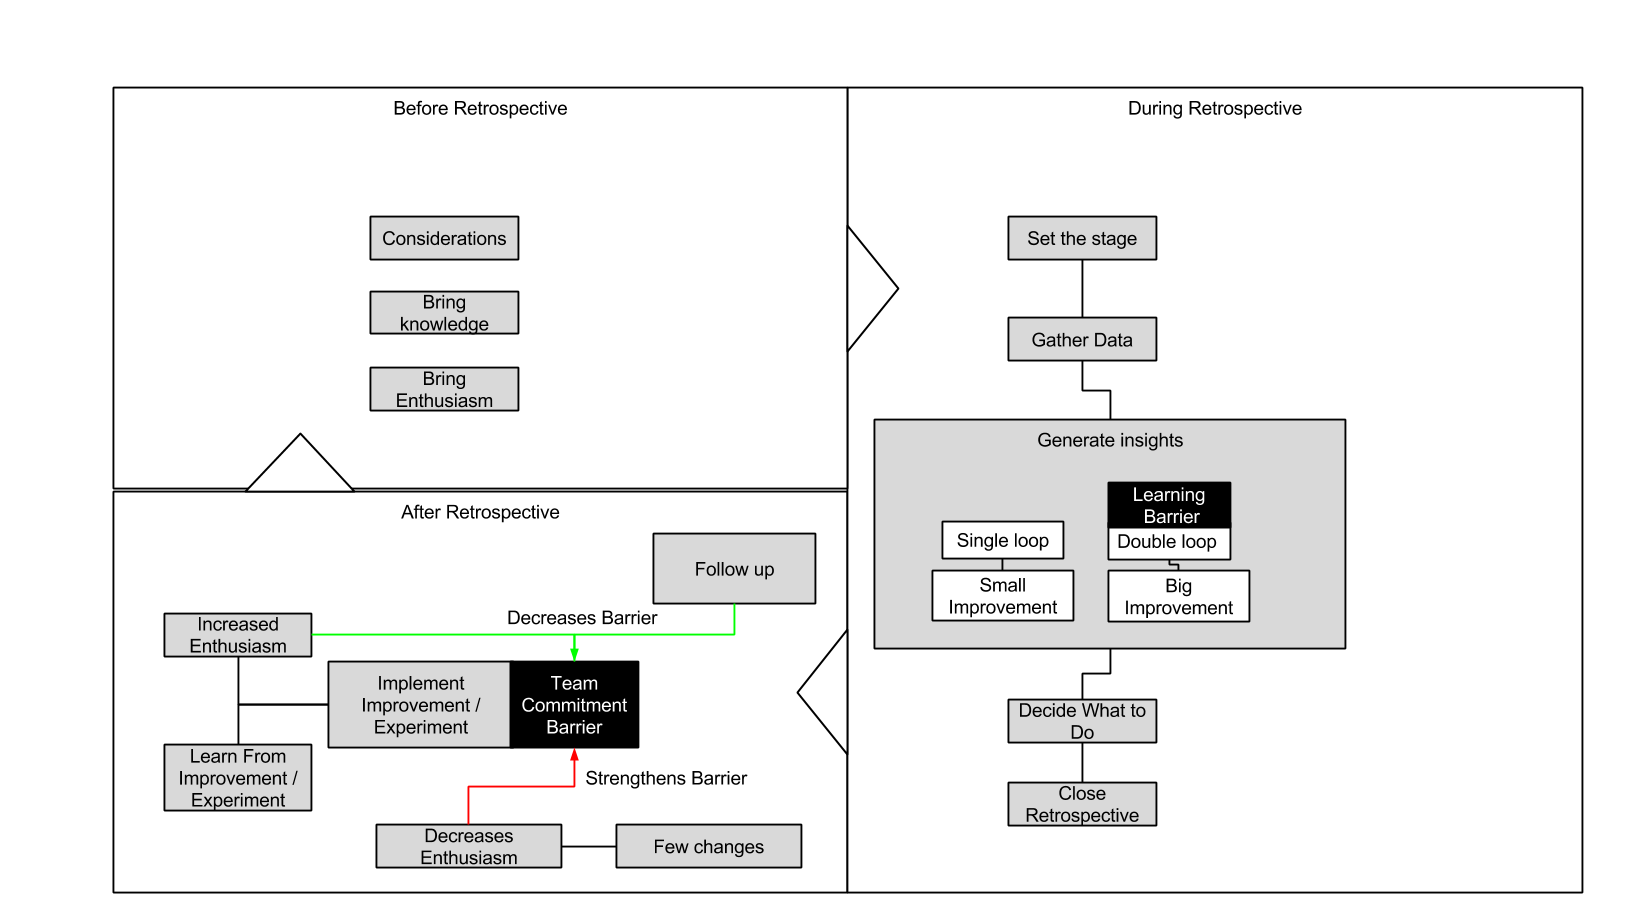
\includegraphics[width=\textwidth, keepaspectratio]{figures/retro-outcome.png}
	\caption{Our perceived state of the retrospective.}
	\label{figure:retro-current-state}
\end{sidewaysfigure}

\afterpage{\clearpage}

\subsubsection{Before Retrospective}
The first part of the retrospective practice consists of three elements that we have been able to see through this study: Considerations, bring knowledge and bring enthusiasm. 

Before the retrospective the facilitator or team is required to bring consider some considerations. Dingsøyr \cite{Dingsoyr2004} proposes several things, however we have seen few of this employed in practice. The considerations we have observed employed by teams today are external facilitator and open or structured discussion. Two of the teams, Echo and Alfa had made the decision to employ an external facilitator. Several of the teams had chosen KJ-Sessions as discussion form, while others just held an open discussion. We have not seen any evidence that any of the teams has made any informed decision on Dingsøyr's considerations. 

Bringing knowledge and enthusiasm is required by the participants before the retrospective. If no one of the 

\subsubsection{During Retrospective}

\subsubsection{After Retrospective}



\subsection{Method Proposal: Meta-retrospective}
\label{section:Method-propsal}
\todo[inline]{Skriv og knytt til egne funn}

\begin{sidewaysfigure}[!h]
	\centering
	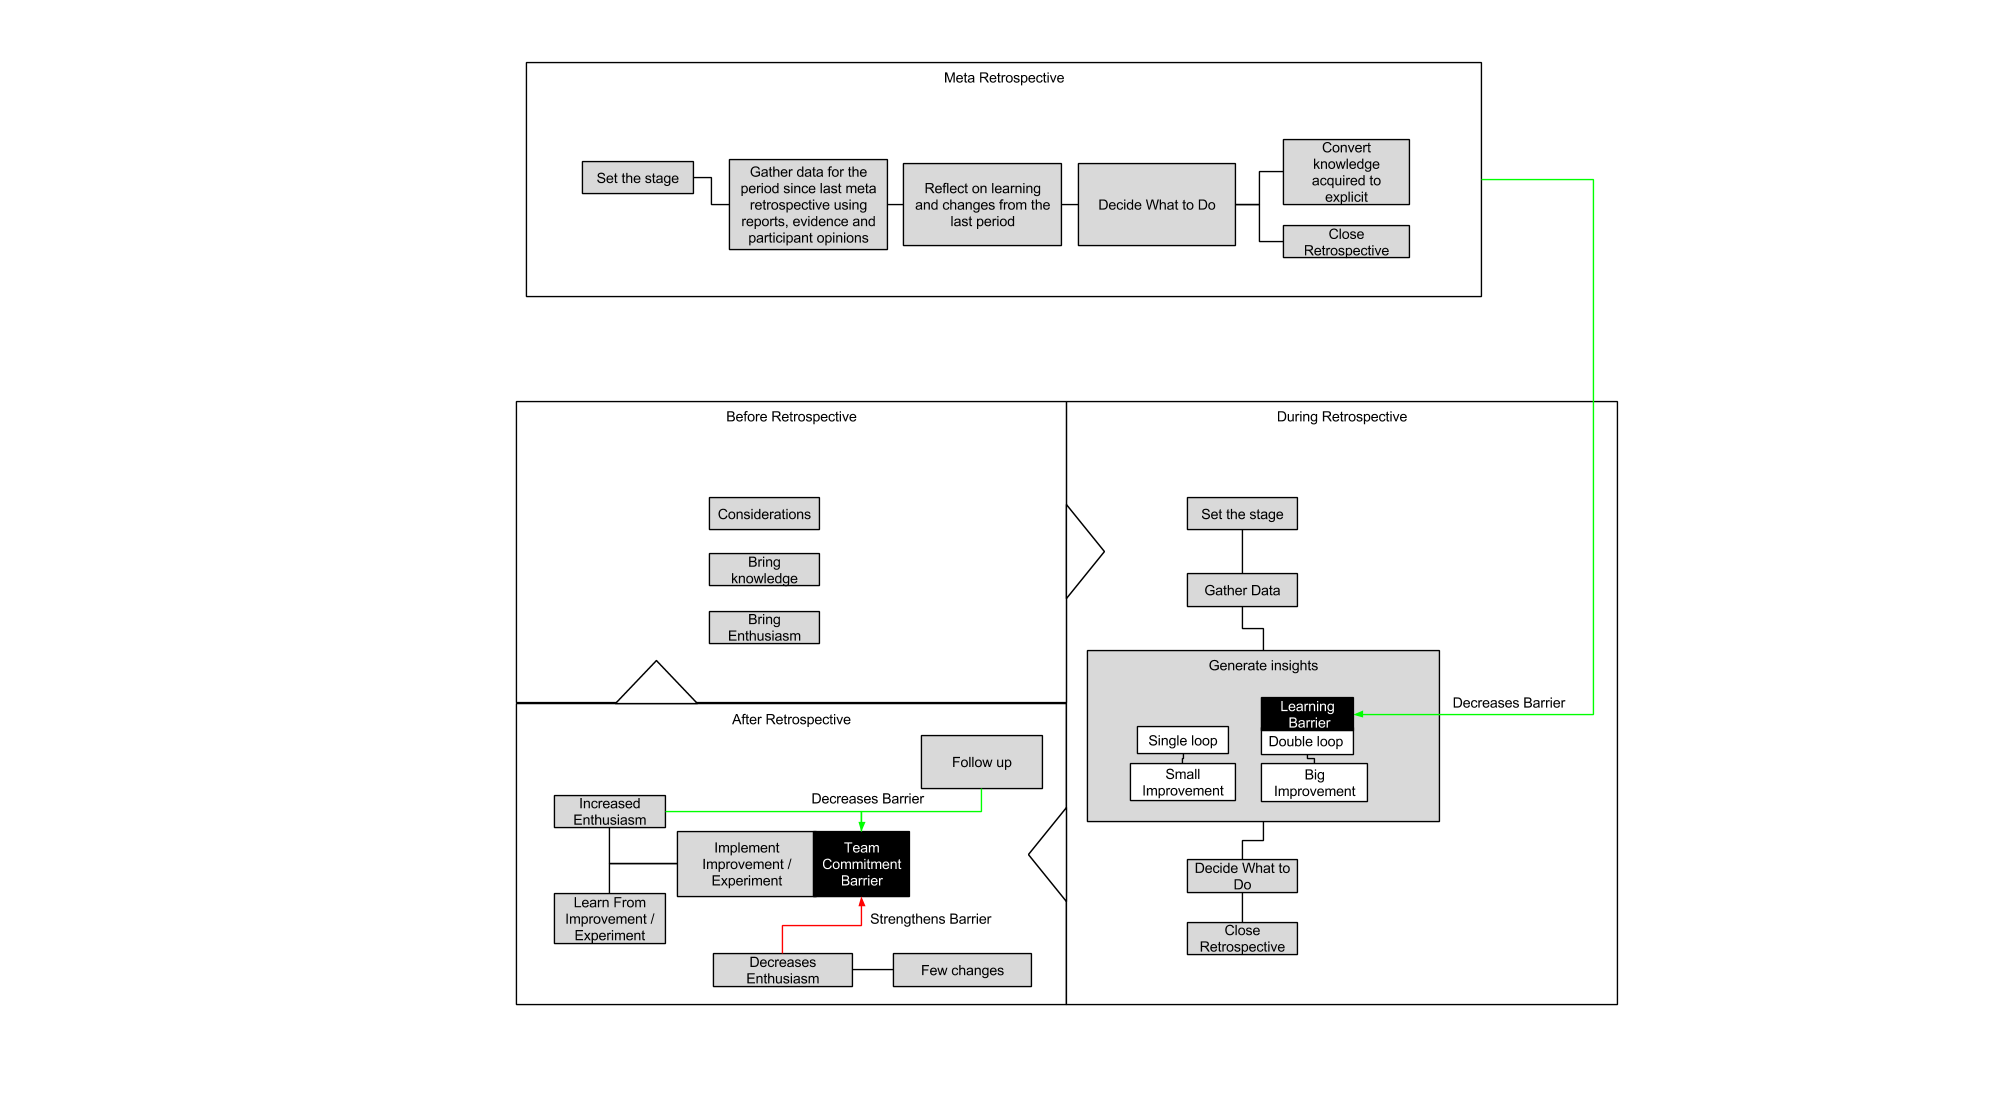
\includegraphics[width=\textwidth, keepaspectratio]{figures/meta-retro.png}
	\caption{Retrospective state after introduction meta-retrospective}
	\label{figure:retro-meta-state}
\end{sidewaysfigure}

\begin{figure}[!h]
	\centering
	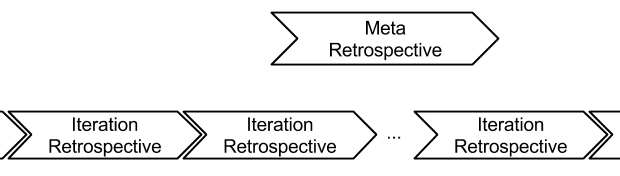
\includegraphics[width=\textwidth, keepaspectratio]{figures/meta-retro-occurence.png}
	\caption{Visualization of meta-retrospective occurrence}
	\label{figure:retro-meta-occurence}
\end{figure}

\subsection{Guidelines for Conducting Retrospectives}

Through this study we have identified several characteristics that we believe will have positive impact on the conduction of the retrospective process in a modern team. These will be presented in a set of guidelines, followed by a short explanation of each point.

\begin{enumerate}
	\item External facilitating.
	\item Implementation of actions 
	\item Address actions to name and visualize
	\item Enthusiasm
	\item Trust
	\item Ownership
	\item Experimentation
	\item Reflection on own learning. (link til meta retro)
	\item Regular retrospectives
	\item Measured varying of technique
	\item Find root causes
	\item Follow up implementations
	\item Reflect on how to conduct own retrospective
	\item Attempt to move beyond day to day tasks
\end{enumerate}

\paragraph{External facilitating}
As described in \autoref{section:facilitator} we observed multiple instances in which the use of an external facilitator was positive to the team. There are multiple approaches that could be used to arrange an external facilitator, an example would be switching SCRUM masters between teams in the company, another possibility would be using personnel from outside the company.

\paragraph{Implementation of actions}
The ensuring implementation of actions appears critical for a team to have confidence and trust in the retrospective process. Therefore attempts to conduct an optimal retrospective should attempt to ensure that actions are completed, and that this success of this is acknowledged by the team. As seen in our work with team Zulu this is very possible and can lead to a positive effect in the team. Implementation of actions feeds the positive loop described in \autoref{section:positive-loop-enthusiasm}.

\paragraph{Address actions to name and visualize}
One step we observed that had a major impact on the implementation of actions was the follow-up protocol. In \autoref{table:follow-up-techique} we observe that the teams assigning name to an action are satisfied with their protocol are satisfied. Another positive step is the visualization of the actions.


\paragraph{Follow up implementations}
A team should ensure that there is some sort of follow up that ensures that actions are implemented. For example this responsibility can fall to SCRUM master as seen in team Echo in section \autoref{question-6}.

\paragraph{Trust}
The building of trust seems absolutely central to unlocking the potential of the retrospective session. Thus a team looking to improve should investigate possibilities relating to increasing the sense of trust between team members. One example of the positive impact this can have on a team can be seen in \autoref{question-21}, where team Delta improves team dynamic through a discussion enabled by the high level of trust in the team.

\paragraph{Ownership}
The generation of ownership has a very positive effect on the team's attitude towards retrospective. This is discussed in \autoref{section:positive-loop-enthusiasm}. In order to facilitate this ownership a team should be empowered in their decision making, leading to them shaping their work processes into something they own.

\paragraph{Experimentation}
A retrospective should be open to leading to experimentation. We have observed this lead to several benefits for the teams in our analysis, this is described in more detail in \autoref{section:experiments-in-work-place}. 

\paragraph{Reflection on own learning}
Through our work we discovered that team level reflection on learning processes has little or no presence. The work done with team Zulu indicates that this reflection can provide benefits, and we elaborate our ideas for this characteristic in \autoref{section:Method-propsal}

\paragraph{Regular retrospective}
Teams without regular retrospectives can be negatively affected in several ways, as described in \autoref{section:Retrospective-timespan}. 

\paragraph{Measured varying of technique}
We got a wide range of answers when we investigated the use of techniques in a retrospective, as seen in \autoref{section:retrospective-practices-used}. Thus it seems advisable for a team to experiment with using different techniques in order to discover what works for them. One should be mindful of too much variation, as too much variation could steer focus over to the technique instead of the retrospective session

\paragraph{Reflect on how to conduct own retrospective} % (fold)
A team can improve by reflecting how they can benefit from established theory, for example considering how they compare to Dingsøyr's approach elaborated on in \autoref{section:Dingsoyr-Approach-Introduction}.


\paragraph{Find root causes}
As described in \autoref{discussion:learning-impediments} some teams can benefit from increasing their focus on double-loop learning. This can lead to more effective decision making as underlying issues are targeted instead of superficial ones. Some techniques observed to find root causes are described in section \autoref{question-13}.

\paragraph{Attempt to move beyond day to day decisions}
Our work has seen that a retrospective have a potential to move beyond operational decisions, this is for example shown in \autoref{section:decision-making-zulu}. A team mindful of this potential is better suited to tailor their retrospective.


 
\subsection{Future Work}

\clearpage

\chapter{Conclusion and Future Work}
\section{Conclusion}
Throughout this thesis we have conducted an empirical study, through a multiple case-study of mature agile development teams, investigating the outcome returned from the retrospective in terms of organizational learning and retrospective characteristics, and thereby answering Dingsøyr and Dybå’s call \cite{Dyba2008} for empirical studies into mature agile development teams.

The studies revealed that todays retrospective practices is approximating an organizational learning II system as described by Argyris and Schön \cite{Argyris1996}. Most of the governing values are already introduced in todays practice. We have seen that single-loop learning is the primary learning occurring, even though double-loop learning is the expected outcome from organizational learning II systems. We have identified one barrier to double-loop learning which consists of several factors. Through our depth study we have seen that reflection on ones own learning helps give focus to the retrospective and lower this barrier and we have proposed a method to help achieve this. 

For the current characteristics of todays retrospective we have seen that the outcome of the practice is improvement opportunities and learning which could result in improved efficiency, increased enthusiasm and adaptation of work-processes, work environment, and product quality. For the processes of the practice we have identified a feedback loop with a barrier for implementation of improvement opportunities, depending on team commitment for implementation and enthusiasm for the retrospective. 

Finally todays retrospective practices provide agile development teams to adapt their current work-practices and enables them to learn from past development iterations and thus provide the means for identifying improvements opportunities and improve from them. 

\section{Future Work}
For future work we would recommend conducting similar studies in other parts of the world to increase sample size and further verify the results of this thesis. Research investigating the method of meta-retrospectives and its value would also help verify this research. Other future work would be to determine the value of double-loop learning to help identify which issues should be identified down to their underlying influences. 
\todo[inline]{Alf shared mental models}
% Include more chapters as required.

\bibliography{references}
\bibliographystyle{plain}
%%=========================================
\begin{appendices}
\chapter{Interview Guide}

\label{section:interview-guide}
\textbf{Purpose:} This interview is designed to be conducted in ~45 minutes, it will focus on organization learning and retrospectives in a project or business. The interview will be recorded and transcribed. \\
\textbf{Participants:} 2 interviewers (Alf Magnus Stålesen and Bjørn Dølvik) as well as a relevant representative from the team in question. For example the SCRUM master of the team, or the person in charge of holding the retrospectives. \\

\begin{center}
	\textbf{General overview}
\end{center}
\begin{enumerate}
\item What is your role?
\item Could you describe your team?
\item How does the team conduct it’s retrospective meetings?
\begin{enumerate}
	\item Frequency
	\item Duration
\end{enumerate}
\item What are the positive aspects that the retrospectives bring to your team?
\item What are the negative aspects that the retrospectives bring to your team?
\item What steps are taken to enforce or follow up on decisions made during the retrospective?
\item Do you have any examples on issues or actions that can hinder the function of the retrospective?
\item What kind of methods are you utilizing, and how would you evaluate them?
\item Do you take any steps to encourage learning? Bonuses etc?
\item As a SCRUM master do you feel like a facilitator or a leader? How does this impact the retrospective?\\

\begin{center} 
	\textbf{Organization learning questions}
\end{center}
\item Has something that has come up during a retrospective that has changed how you work or think?
\item Do you use any special information to assist in decisions? What kind of information is this and what value does it have? Tools etc.
\item Do you solve problems during retrospectives or do you take steps to investigate the root cause of the problem? Do you have any examples of root cause identifying?
\item Are there any obstacles which makes it difficult to take decision and prohibits learning?
\begin{enumerate}
	\item If so which?
\end{enumerate}
\item Does the team reflect on how you learn?
\begin{enumerate}
	\item If so how is this done? And is this spread further into the organization.
\end{enumerate}
\item How do you learn from retrospectives?\\

\begin{center} 
	\textbf{Team dynamics questions}
\end{center}
\item What is it about your team, that makes you able to learn through the retrospective?
\item What in your team could be improved to further enhance the learning through retrospectives?
\item Do you have any experiences where norms and cultural differences have an impact?
\item Which properties in the team do you see as positive or negative? How do they influence the retrospective?
\begin{enumerate}
	\item Are there someone in the team who uses a lot of the time during the retrospective? Why and how does it influence the retrospective?
	\item Are the someone in team who rarely contributes during the retrospective? Why and how does it influence the retrospective?\\
\end{enumerate}

\begin{center} 
	\textbf{Anything else}
\end{center}
\item Do you have any examples of major breakthroughs or development that has happened through team learning?
\item Is there anything we haven’t covered, that you feel is important for us to know that is related to how your team work with retrospectives and the knowledge learned from it?
\end{enumerate}

\chapter{Pilot Analysis}
\label{pilot-analysis}
Settling on tabulations as our means of content analysis the different categories had to determined. We performed a pilot study.
The pilot study was conducted in order to investigate the potential of analyzing a set of the 77 retrospective reports.  The pilot study was limited to 11 reports, where we picked every 7th retrospective chronologically. This distribution was chosen in order to get an even spread to represent the whole set, as well as keep the size manageable for the short preliminary study.

The pilot study analysis lasted for one week, and included agreeing on the parameters and methods for the study, as well as a short workshop session where the results were presented in front of a group of fellow researchers. This workshop session consisted of a short presentation of the findings of the study. After the presentation we had a brainstorming session where we received feedback on potential improvements, as well as general impressions. 

\begin{figure}[!h]
	\centering
	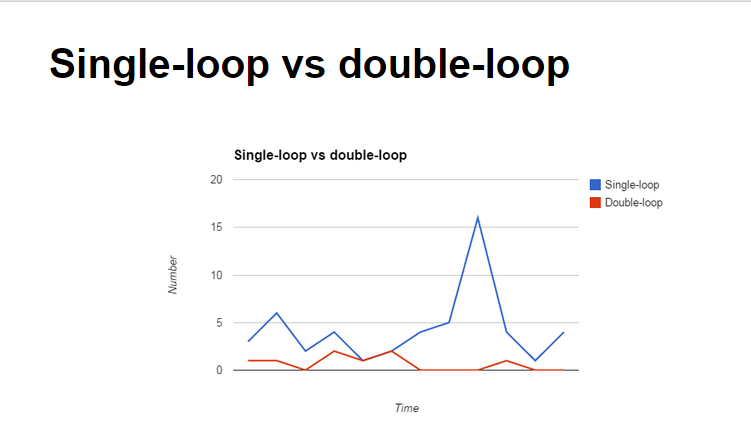
\includegraphics[width=\textwidth]{figures/Pilot_loop.PNG}
	\caption{An example of a slide from the pilot study presentation }
	\label{figure:Pilot Slide}
\end{figure}

\chapter{Content Analysis Categories}\label{appendix:categories}
The results of our pilot analysis gave us an extended set of categories that we will now describe further. Mainly we found six main themes that we could derive categories from. The six themes were: Nature, Context, Decision Making, Organizational Learning, Development and Management. We will describe each of these themes and their set of categories further in the sections below.

\section{Nature}
The nature of the action is the first theme that the content analysis is going to inspect. We define the nature of the action as how the origins of the action began. Did they come from a problem that occurred during the iteration or is it a continuation of something that has been working well in the past. Through our analysis we will try to understand the origins of the actions and classify them either as positive, negative or undefined. We define our classifications below. 
\paragraph{Positive} Positive actions is those actions where the origins of the action is in a positive context. If the action represents a current good working practice being continued, or something uncommon happened that gave positive results, it would be classified as positive.
\paragraph{Negative} The negative actions are those actions that has its origins from a problem or abnormal issue resulting in negative results. If an action is a result of a problem or abnormal issue it is classified as an negative action. 
\paragraph{Undefined} In the cases where it is unclear whether the origins of the action is positive or negative we classify the action as undefined. Such occurrences can be a result of missing context or actions that seem to have neither positive issues or negative issues as its origin. 

\section{Context}\label{method:context}
The context surrounding the action will be analyzed. The context off the action is based on the underlying issue that leads to the needed action. We divide the issues into three main categories, technical, process and undefined. 
\paragraph{Technical}
A technical issue can be a issue relating to technical competence, bugs or problems.
\paragraph{Process}
A process issue stems from a problem with a process, or potential for improvements in the existing processes. This can for example relate to communication between colleagues or work scheduling.
\paragraph{Undefined}
 An undefined issue might not have any clear origin, or might be too loosely described to be classified easily.

\section{Decision Making}
Rational decision making is how decision makers should think and should act based on coherence and rationality, according to M. Drury et al. ~\cite{Drury2012}. N.B. Moe et al. ~\cite{Moe2011} appends bounded rational decision-making as the means of understanding how decision making is made in non-routine activities. N.B. Moe et al. reasons that both are needed when analyzing decision-making in an agile context:
\begin{quote}
Software development involves both routine and non-routine activities. Hence, it makes sense to use both rational and bounded rational decision making theories when explaining decisions in software development processes. 
\end{quote}
Drury et al. distinguishes between two types of decisions being made in an organization, the strategic and the tactical. Moe et al. distinguishes between three types: Strategic, tactical and operational. We will use the three-type model. Each decision type will be described in the following paragraphs. 
\paragraph{Strategic}
A strategic decision is a wide ranging decision dealing with multiple or sizable issues, often causing major changes and have a long term impact.Moe et al. describes the strategic decisions as the following: 
\begin{quote}
Strategic decisions are related to organizational goals and objectives. The information concerning such decisions is usually incomplete and the decision-making process may extend over a considerable period of time.
\end{quote}
The actions that are categorized as strategical is the ones that proposes changes that have a long term impact or proposes changes that are related to the organizational goals. 
\paragraph{Tactical}
A tactical decision is smaller than a strategic decision it seeks to deal with the distribution and use of resources available to the team. Moe et al. described it as: 
\begin{quote}
Tactical decisions are related to identification and use of resources.
\end{quote}
All actions that specifically proposes to identification of resources or proposes changes to how resources are spent will be classified as tactical.
\paragraph{Operational}
Moe et al. describes an operational decision as: 
\begin{quote}
Operational decisions deal with ensuring effectiveness of day-to-day operations within the organization. 
\end{quote}
Every action that are restricted to only day-to-day operations will be classified as operational decisions. They might be quick fixes that solve a single problem. 
\paragraph{Undefined}
An undefined decision might be difficult to categorize because of a lack of context or an unclear description.

\section{Organizational Learning}
Organizational learning is a process where an organization takes steps to improve its current work environments by reacting to issues that arise. These steps can be varied, and we divide them into single-loop, double-loop and undefined. Retrospectives have a central role in 	organizational learning, as described by Dingsøyr ~\cite{Dingsoyr2007}
\paragraph{Single-loop}
A single-loop action is an action designed to change or tune a process in order to improve it. The action does not seek to address underlying problems, and are a single-feedback loop from observing an issue to making a change. A retrospective can facilitate single-loop learning where the project team uses the input during the retrospective to make adjustments to their current work ~\cite{Dingsoyr2004}
\paragraph{Double-loop}
A double-loop action is designed to solve an issue, as well as address the underlying cause of the issue. This requires an understanding of the underlying issue and the nature of its influence. Double-loop decisions can be facilitated through a retrospective, often these are as a result of a more drastic need for change and an understanding of the underlying problem. ~\cite{Dingsoyr2004}
\paragraph{Undefined}
An action might not be clearly described, or the nature of the action can not be interpreted. We will classify these actions as undefined.

\section{Development}
An issue that is related to the development of the product is included in this category. The development process is the actual work performed to create the product, as well as processes directly related to this work. The different categories included in development were chosen after discussing with advisors, as well as personal experience from the writers
\paragraph{Development}
Development includes the writing of code, specifying requirements, construction the system architecture and other aspects of designing of the system. 
\paragraph{Planning}
An action that is categorized as planning is when the action is suggesting changes to planning in future iterations or is a result of an issue occurring in a former iteration. Estimations, task-prioritization, scheduling and etc. all goes under the planning category.
\paragraph{Testing}
Issues related to the testing of a product, this includes unit, module and system testing. Issues related to testing can also be communication between testers and developers.
\paragraph{Documentation}
Action that are categorized as documentation is those that are related to the documentation part of developing a system. Typical actions are those that describe or propose changes to documentation practices. This can also include tutorials that explains the product and improves usability. 
\paragraph{Builds}
During development of a software system building the software system can be a tiresome task. The actions that are categorized as builds are those who proposes practices that changes the current build practices.
\paragraph{Release}
When a system feature or a part of a system is finished, usually at the end of an iteration, one deploy the new part of the system into production, available for the users. For the actions that categorized as release, the action describe some aspect of the release practice and either proposes changes or suggest new practices.
\paragraph{Business}
Business development is a critical part for an organization to create profit. Software system often can save costs and create new business opportunities and as a part of a software development team one also has to consider business perspectives. We categorize all actions that are related to business development or proposes some business related changes as business. 
\paragraph{Undefined} If an action is neither of the development phases described above we classify it as undefined. 

\section{Collaboration}
One of the aspects during a software developing process is collaboration. Fægri ~\cite{Faegri2012} describes collaboration as the following: 
\begin{quote}
Collaboration is a key aspect of software development. Collaboration allows groups of software practitioners to deal with uncertainty, complexity and interdependence. And in dealing with these challenges, the group demonstrates its collective problem-solving ability.
\end{quote}
Through our pilot analysis we registered several activities that are related to collaboration. Communication, leadership, competence, external relations and planning all belongs beneath the collaboration banner, and we describe in detail how we classify each of them below. 
\paragraph{Communication}
Communication is a widely used word and concept, but it rarely is defined. By using Merriam-Webster dictionary ~\cite{MerriamWebster2015} we found a definition that can serve as a clarification: 
\begin{quote}
The act or process of using words, sounds, signs, or behaviors to express or exchange information or to express your ideas, thoughts, feelings, etc., to someone else.
\end{quote}
Nakakoji et al. ~\cite{Nakakoji2010} distinguishes between two types of communication related to software development, coordination communication and expertise communication. The first one being the process of coordinating the development activities and the last one being when a developer obtain some information regarding a software artifact, either through code comments, wikis or other means. 
We are however not going to distinguish between these two communication types in our content analysis as we believe the two differentiations is covered by the context of the action as described in \autoref{method:context}. For our content analysis we are simply going to count every instance of communication for every action that is related to communication between team-members regardless if it is through text, speech or other means of communication.
\paragraph{Leadership}
As is the case with communication, leadership is also widely used concept, that is rarely specified. Again we turn to Merriam-Webster \cite{MerriamWebster2015} for a definition: 
\begin{quote}
The power or ability to lead other people.
\end{quote}
Agile development teams is often self-organized as it is one of the principles in the agile manifesto \cite{AgileManifesto2015}. This can result in no clear leadership. For our content analysis we are going to consider decisions and guidelines set by the group itself as leadership activities. We categorize actions as leadership if they somehow suggests changes to leadership or if the actions is a result of some leadership related issue. 
\paragraph{Competence}
We define competence as the ability to perform a certain task in a adequate quality. Each member within an agile team has their own set of knowledge that they use to solve different tasks. If any issues arises and the group is lacking the knowledge to counter it we categorize the action created to resolve it as an competence action. An example could be issue of lacking the knowledge resolving a database error and the action is to send one developer at a database course. This action would then be categorized as an competence action.
\paragraph{External Relations}
By the category external relations we mean if the team has any actions that is a result of issues arising from external factors or the actions that team is creating to inflict some external factors. Example of external relations can be customer relations, communication with server maintenance team or other development teams.   
\paragraph{Undefined}
For those actions that the origin is unclear and the goal is not related to any of the collaboration categories we categorize them as undefined.

\chapter{Shared Mental Models}
\label{section:mental-models}
The theory of shared mental models is from cognitive psychology, and can be used as a lens to evaluate agile development and methodology as described by Petter et al\cite{Petter2013}. The concept is that a team has a shared mental model that is central to the mutual understanding between team members, and thus essential to project success. Without a good shared mental model a team is left with a poor understanding of the task at hand, as well as barriers for cooperation. Two metrics used to measure a team's shared mental model are ``similarity'' and ``accuracy''. Where ``similarity'' is the degree which the shared mental model is similar between team members, and ``accuracy'' is the degree which the shared mental model matches objective measures. 

\section{The stages of Shared Mental Model generating}

\label{section:mental-models-stages}
	
Four different stages of building shared mental models are identified \cite{Petter2013}. These are knowing, learning, understanding and executing. An overview of these stages is seen in  \autoref{table:stages-mental-model}. Knowing is the stage where a team gets exposed to information relating to their project and project goals, at this stage team members are encouraged to share information between each other. The second stage is the learning stage, this stage consists processing the information gained in the knowing stage. The understanding stage is defined by reaching consensus and understanding the team member's individual views. Executing is the last stage, with a developed shared understanding the team is able to reach goal, at this stage a team responds to a situation based on the work done in the previous stages.

\begin{table}[!h]
	\begin{centering}
	\caption{Four stages of mental model building}
	\label{table:stages-mental-model}
	\begin{tabular}{l | p{0.7\textwidth}}

	\hline
	Stage & Description \\
	\hline
	Knowing &  Information exposure and sharing\\
	Learning & Information processing \\
	Understanding & Consensus and common ground \\
	Executing & Shared understanding and  \\
	\hline
	
\end{tabular}
\end{centering}
\end{table}

	
\section{Shared Mental Models and retrospectives}

Petter et. al. \cite{Petter2013} describe multiple agile development practices, but do not focus a lot on the agile retrospective. In the appendix of the article they give the following link between retrospectives and shared mental models.

\begin{quote}
Enhances the development of learning and understanding stages by facilitating the information sharing and integration. This practice also improves the teams’ executing capability in the next sprint
\end{quote}

The shared mental model practices that are involved in the retrospective are identified as self corrective, training and reflectivity. We discuss the relationship between our results, retrospectives and shared mental models in \autoref{section:shared-mental-models-discussion}.

\chapter{Transcription: Interview SCRUM Master - Team Zulu}
Researcher 1: Vi er interessert i hva du tenker som scrum master først og fremst. Hvordan du opplever ting, samt elementer fra presentasjonen også om det var noe som overrasket eller noe du savna.

SCRUM master: Ja altså det var jo interessant, vi jobber med dette hele tiden. Vi har ett veldig sterkt forhold og eierskap, men vi har aldri gjort dypdyk eller kategorisert de forskjellige ... tiltakene. Så det var veldig interessant å se  at liksom trendene, det er ting når man liksom har en følelse av hvordan det ser ut, men det er en annen ting å se det i en graf. Jeg hadde visste ikke helt hva jeg skulle forvente, jeg visste jo litt siden jeg hadde snakket med dere, så jeg visste nok mer enn de andre, men jeg synes det var veldig bra, veldig interessant.

Researcher 2: Glimrende, nevnte det om trender da, og det er jo noe vi er redde for å uttale oss om, vi skjønner jo at dette bare er en liten del av bildet. Men i forhold til hvordan vi forklarte vår tankegang, gi det mening når du så det i det store bildet da?

SCRUM master: Ja, altså dere klassifiserer så teller dere og så ser dere om det er en trend. Type sånn scenario template da så er det et virkemiddel på en måte, noe som vil dukke opp i all slags kontekst, som et virkemiddel vi bruker for å gjøre de rette tingene. Da var jeg jo overrasket om at det flata ut, men det kan jo være tilfeldig og. Det finnes mange virkemiddel for å få gjør ting, men det var jo påfallende at flere grafer flata ut tidlig på året i fjor og det sammenfalt jo da med diverse ting som har skjedd i vår avdelig, jeg har tro på at der er det en korrelasjon altså. Det er en sammenheng da, vi vet jo at dette er litt guesswork, kjenner jo ikke alt, kjenner ikke 100\% bakgrunnen til ting som dukker opp i retrospektiv, dere har jo gjort en fantastisk jobb.

Researcher 2: Nevnte jo det jo tidligere, men akuratt denne typen studie har ikke blitt gjort før så det er jo litt interessant for å se anvendelse område og hva tenker du om det som ett statistisk verktøy til analyse osv? Du nevnte om å ha det som ett dashboard?

SCRUM master: Poenget er at vi bruker jo vårt eget system, det som vi utviklier det som vi lever som produkt, det bruker vi internt for å regisstrete alle slags retrospektiver vi har, så lager vi ny sak og så lager vi actions og det har vi jo gode muligheter for å få ut statistikken. Og hvis vi hadde bare klassifisert det slik som dere gjør så kunne vi fått ut statistikken på ett dashboard, vi har andre dashboard der vi teller kommunkiasjonsfeil og trender der da, med forbedringsforslag fra kunder. Så vi kunne definitivt gjort det, det som gjør at jeg er litt skeptisk i utgangspunktet. Det som gjør meg litt skeptisk er at vi har hatt verktøy tidligere der vi har vært nødt til å fylle ut klassifisering, obligatoriske felt som man ikke kan lagre uten å fylle ut denne klassifiseringen da. Og av og til blir det litt i hu og hast litt tilfeldig valgt man har for eksemple causes, da man ikke har tid og det er grunnen til av feilen oppsto, man finner ikke den rette og kvaliteten blir dårligere, uansett så har vi ikke brukt det til noe. Vi har egentlig brukt det til arbeid til å få det riktig, men har ikke tatt ut statisitikken og brukt til noe fornuftig, og da er det waste, invistert tid som vi ikke får noe glede av. Men det jeg tror med noe tilsvarende for tiltak for retrospektiv så måtte vi passet på at vi faktisk brukte det til noe, og det er jo interessant å se, men når man måler seg selv og man har ett target og du vil nå en target og du vet at det blir målt så kan det jo påvirke det som blir sagt i retrospektiv, selv om man sikkert ikke ønsker det kan det likevell påvirke, jeg vet ikke det er litt både og. Men det hadde vært utrolig kult å få hatt litt hånda på pulsen og se hva vi gjørl

Researcher 1: Sånn som nå så har dere dette prikkesystemet, merker du noe tension på det?

SCRUM master: Ja det blir jo veldig synelig da hvis man slite litt, men det er jo hele poenget, hvis ett scenario henge på samme plassen og får prikk på prikk så er det om å gjøre ett eller annet tiltak siden det er ett eller annet problem da. Det var jo det som var ideen, nå så du jo denne ``testing'' har vært der ganske lenge, og da vet vi jo hvorfor, det var jo mye tester, over 100 requirements, da sier det jo seg selv. Men man merker det jo hos noen team members at det er litt sånn at det ligger litt synlig, men vi gjør det jo ikke for at det skal være en irritasjon men for å synliggjøre det. Da må vi gjøre tiltak, og egentlig kan det vær ett konrekt, og det er synliggjort men det er blokka. 

Researcher 2: Hvis du liksom i det ideele, har du noe du skulle ha med ressurser eller tid noen forbedringer på den eksisterende formen på å holde retrspektiver?

SCRUM master: Jeg nevnte tidligere at det er veldig enkelt sånn vi gjør det  og grunnen til det er at alle skal få en sjanse til å si noe, hvis man bare sitter løst og snakker om det så er det noen som vil gripe ordet. Og det dekker jo behovet sånn sett, men det finnes jo andre metoder for å utføre en retrospektiv. Vi hadde jo en liten demo nå på forskjellige teknikker, blant annet dette her med positive og negative ``Hva synes dere har vært positivt og hva synes dere har vært negativt?'' Hadde hele tavla full av lapper, skulle lage en sånn ``weather forecast'', det ble vi egentlig enige om at vi skulle innøre, altså ikke hver iterasjon, men ett par ganger i året. Det var interessant å se hva vi liksom fikk ut av det, men vet ikke vi har ikke egentlig ikke noe som kommer til kort i det vi har vi får frem det som, det er veldig viktig at man føler man blir tatt vare på og at man blir hørt, hvis man snakker og det er ingen som tar hensyn til det man sier, da er man dømt og man gidder ikke bidra til slutt. Føler vi har fått en kultur der alle føler de har noe de skulle ha sagt da.

Researcher 2: Det vi har lyst å ta noen eksempler på, at noen føler at man ikke blir tatt på alvor kan bli en negativ feedback loop der folk bidrar enda mindre og så blir enda fortere ferdig.

SCRUM master: I en travel hverdag så er det ikke alltid det passer, derfor bruker vi en time og ikke noe mer, så ofte så blir det sånn at vi kutter og tar det på neste om 3 uker, men likevell den timen i en travel hverdag kan være litt forstyrrende, men hvis vi ikke gjør det så.. vi utsetter, dropper det denne gangen så neste møte varer jo mye lenger, så folk har jo noe de vil ha sagt, så vi har konkludert med at vi måte være strenge på dette. Og har hver 3 uke. Jeg tror folk tror det er positvit. Hva spurte du om egentlig?

Researcher 2: Om du hadde noen potensielle forbedringer?

SCRUM master: Ja, nei jeg er jo egentlig fornøyd med sånn som vi har det, har ikke fått så mye input, hadde jo besøk fra sintef men det er noe vi kan gjøre nå og da i tillegg, men vil ha denne basci formen

Researcher 2: Du nevnte at noen for noen kan det være ett forstyrrende element i en travel hverdag, er det noe fokus på at det skal være en positiv opplevelse, flerne artikkel foreslår gratis lunsj eller lignende, hva slags tanker har du? Altså skape litt sånn ``festelig'' atomsfære.

SCRUM master: Det er jo egentlig ett godt poeng da, det kunne vi sikker gjort noen grep for at det skal være positivt altså, det skal jeg tenkte på. Sånn i den formen det er nå så prøver vi å ha en lett og ledig tone der vi spøker litt og ler litt det skal ikke være gravalvorlig, men noen ganger  så går diskusjonen og man har forskjellige meninger det som og gjerne kjennetegner våre diskusjoner er at vi prøver å finne consensus på en måte, og hvis man ikke blir enige så prøver vi dette og hvis ikke det går så kan man prøve noe annet senere. Men akuratt noe positiv aura rundt det... Hva har andre gjort?

Researcher 1: Noen har gratis lunsje og lignende.

Researcher 2: Noen hadde farger og stjerner til de som var flinke.

Researcher 1: Noen brukte kaker eller lignende for at man skulle forbinde det med noe positivt, det er jo mange som sliter med, mange som ikke har en positiv følelse.

SCRUM master: Ja at de ikke helt ser poenget med det. Det er noe man blir pådyttet på ett hvis, ja mitt inntrykk er at vi deler eirerskapet, og man liksom føler eierskapet.

Researcher 2: Rent akademisk, det vi snakket om med fri lunsj osv, det at man føler det positivt, hensikten er ikke bare å si at man følte dette fungerte bra, men det er også at det blir en klapp på ryggen ``bra at vi får til dette maintenance møtet". Så tenker man neste gang man skal på retrospektiv møte, ``det vi gjorde for 2 ganger siden funka" Så blir man gira for neste. Hensikten er jo  at folk skal engasjere seg så mye som mulig.

SCRUM master: Jeg ser den altså, det er ikke noe sånn organisert, typisk de som var involvert i den endringen vil gjerne si hvordan det var, og det funker kjemperbra, vi kunne nok vektlagt det mer. Sende ord videre liksom, man kan jo spør om det er noe positivt liksom,

Researcher 2: Særlig sånn her problemløsning i team, er jo veldig problemfokusert her, negativet  er kanskje litt lada ord i forhold i den sammenheng at det nødvendig er noe dumt.

SCRUM master: Det er jo negativt til man finner en løsning, da er det noe positivt igjen, når man sliter... f.eks dette med bugs og sånne generelle bugs det kan bli litt liggende og slenge. Vi hadde ett system der man skulle jobbe med det, men det ble ikke noe håndfast og man dedikerte ikke tiden til det når vi fikk den dagen, som var ett veldig enkelt grep, som har vist seg å funke veldig bra, vi ser på statistikken og at dette virker, og det blir en seier da og vi ser det er noe positivt i det. 

Researcher 2: Nå hørtes jo det ut som noe dere er veldig klar over, men hvis man skriver det ned og sier det høyt i gruppa så gir det mer trøkk.
Researcher 1: Vi gikk jo at i fjor hadde dere en(medarbeider) som gjorde at ting ikke helt funka og at retrospektivet ble litt sån taust, og det har vi egentlig fått høre nok om, men har du noen andre tilfeller hvor enkeltpersoner kan være destruktive for retrospektivet?

SCRUM master: Ja jeg skjønner hva du mener det er jo generelt i team da, i agile der man ønsker liksom at teamet skal ha noe de skulle sagt så, sånn at man føler at man bidrar, da er det jo noen som kan ta helt over. Det er ett moment, men det har jo gått bra, det er jo noen i teamet som har mer de skulle ha sagt enn andre. Men tror vi har funnet en vei. Bekymringen er jo, sånn generelt, at man skal bli arrestert hvis man kommer med noe, men det er såpass mye respekt mellom teammedelemene at det går greit, det som var saken, med han som slutta var jo det at han forårsaka så mye misforståelser og problemer at det overskua alle andre problemer. Det var i grunnen elefanten i rommet, det er jo klart alle nyansettelser eller folk som slutter eller hva det skal være alle forandringer i gruppa vil jo forandre dynamikken, da må man liksom finne en ny måte å inrette seg på. Det er jo et interessant spørsmål. Det er vell det beste eksempelet jeg kan huske.

Researcher 1: Er det noen som er veldig stille?

SCRUM master: Det er det, helt klart. Og de komme jo med sine ting de og, men det er bare det at har ikke behov for å markere seg i rommet når de får ordet så har de jo kanskje ting som de har tenkt på. Jeg har jo tenkt på det. At de ikke skal være helt for sakte. Det er jo en ting som ikke nødvendigvis ikkke skriker ut, men jeg føler jo at de bidrar

Researcher 1: Føles ikke det destruktivt eller hindrer ikke fremgang?

SCRUM master: Nei, eller jeg vet jo ikke dette 100\%, jeg går ikke til de og annonsere.. de sa ingenting de som ikke bidro, så måtte jeg vite hva det var.

Researcher 2: Men det er liksom innenfor rammene så er det greit.

SCRUM master: Ja folk er jo forskjellige.

Researcher 2: Det er ett par vi snakket med under lunsj, med han dere hadde problemer med så nevnte de en del sånn der kulturelle forskjeller som førte til problemer da. Har du noen mulighet til å uttale deg om det?
SCRUM master: Ja det har jeg, det er jo åpent. Jeg tror alle i teamet er klar over det, vi har jo snakket om det og, vi har jo.. noen kulturer ønsker å ha alt skriftelig med fem signaturer liksom, og et må inn med teskje. Det er ikke sånn vi jobber,det er ikke sånn vi jobber, vi speccer det er ganske sånn lauslig (løst) Får en handover fra arkiteteken går jo gjennom det så får vi en forståelse og tar litt underveis og da er det jo selvfølgelig en periode i begynnelsen før de blir vant me dette føler jo at de drive jo litt med god arbeidskultur og god skikk. En annen ting er jo tap av ansikt hvis ikke man forstår noe, og det er vi jo helt avhengig av. ``Forstår du ikke hva jeg sier til deg?" ``Ja jeg gjør jo det" og så er det åpenbart etterhvert at det var ikke forstått, man forsto ikke. Trenget du hjelp? og så trenger man ikke hjelp. det fungerer jo godt i Norge da. Det er jo litt det å være off da.

Researcher 2: Nevnte jo det at man ikke hadde lyst å være frekke foran denne personen under retrospektivene da.

SCRUM master: Ja det blir jo veldig personlig, det er jo det som er liskom. Det går liksom på personlighetstrekk og på... Retrospektiv er ikke skapt for denne type ting, det må håndteres på ett annet nivå.

Researcher 2: Det som gjør det for oss er jo det at en personalsak kan påvirke enn annen prosess, det er jo det som gjør det interessant for oss.

SCRUM master: helt klart.

Researcher 2: Nå skal jeg ikke legge ord i munnen din, men si dette problemet med medarbeideren da, tror du at det fantes ganger der de ikke gadd å ta opp andre ting heller, siden de tenker, vi får uansett ikke løst det store problemene, så kunne vi kanskje tatt dette og.

SCRUM master: Det er sånn! Det overskygger. Det er litt sånn,

Researcher 1: Store problemer overskygger de små?

SCRUM master: Ja det er generelle ting. Da blir all fokus på det problemet de mindre trivielle problemene dukker ikke opp før man har løst de andre. Nå var jeg i permisjon når det storma som verst, så har likom blitt fortalt hvordan det var. Det var jo... En ting var at det ikke funket å godt under retrospektivet, men det tærte jo på teamspiriten generelt. Det er jo nok bare ett symptom på ett underliggende problem at retrospektivene ikke funker. Men det er jo klart, det så ble gjort i kulissene er jo at den som fikk personalansvar fikk jo beskjed om alle problemene, og det var opp til ha å gjøre tiltakene, men det er jo ikke så veldig enkelt. Man vil jo helst få det til å fungere.

Researcher 1: Hvordan, store problemer, hvordan takler dere det, hvis de kommer opp på retrospektiv, hva gjør dere da? Setter av tid eller?

SCRUM master: Ja, det kan vi gjør, men for meg dukker de opp før retrospektiv. Hvis det er veldig.. så tar man jo tak i det der og da. Det som vi og kan se er jo for eksempel at vi hadde ett scenario der vi hadde problemer, der det var litt kommunikasjon, og det var litt diverse sånn der, mellom testere og utvikler, nå har vi laget ett retrospektiv kun for de som var involvert og så skal vi sette og ned og finne ut av det. Det blir litt ad hoc. Tenkte jo at vi skulle ta det opp som ett vanlig retrospektiv. Men det er bedre at vi bare tar det det gjelder og så heller deler vi det vi finner og deler med alle.

Researcher 1: Hva skal til for at noe blir tatt opp? Må det vært snakka om før?

SCRUM master: Nei, det er ikke sånn. Noen er veldig flinke og noterer underveis og lager seg en liste om ting de vil snakke om. Mens andre er litt sånn hva var det jeg gjorde siste uke og må tenke etter liksom. Det er sikker og personlighetsforskjell da, noen er veldig metodiske og andre er mer ad hoc, på sparket. Men det er jo... egentlig så har vi, vi ønsker å fokusere på prorsess, det er jo det som egentlig er hovedfokuset, men vi har ingen grenser for hva vi kan snakke om, det blir  litt sånn klassisk team.

Researcher 1: Ja forsåvidt, føler du at teamet er ærlige eller trygge på hverandre gjør du noe for å fasilitere trygghet? 

SCRUM master: Ja altså, jeg føler at de er trygge på hverandre, de fleste har jobbet lenge sammen, men det er. Jeg ser. Et annet eksempel på at kjemien ikke har vært så god da, det var en som for stund siden, det var alltid en greie mellom han og testeren da, det ble liksom personlig fant man en bug så ble det. Åh nå fikk jeg en bug på meg igjen liksom. Følte at han måtte forsvare seg på en måte, og da ble det mye gnikkinger på det mellom testeren og han der utvikleren da. Men da blir det liksom en personssak. og det er sånn som ikke dukker opp i type retrospektiv, men det blir mer sånn som kommer frem gjennom linjene, man snakker i generelle ordlag mens egentlig så snakker de om hverandre.

Researcher 2: Det blir lit sånn passivt aggressivt. 

SCRUM master: Ja, og det er ikke bra, men det er jaa, jeg føler at de aller fleste er ganske åpne med hverandre og snakker direkte med hverandre om det er noe som ikke funker, derfor er det og... altså eneste er kanskje hvis du kommer for en annen kultur der du føler at du ikke skal motsi de du oppfatter som ledere på en måte, så blir du usikker på om de er enige eller om de bare later som.

Researcher 2: Det finnes litratur som sier at et retrospektiv ikke bør ha med ledere folk som har autoritet da.

SCRUM master: Ja, men vi er jo Norge da , og vi er veldig flate i utgangspunktet nordmenn har ikke respekt for lederene sine, det er jo den store fordelen, med å ha de med er jo at når man gjør beslutninger er jo at, Jan Edvard, da kan man jo ta større avgjørelser og trenger ikke sjekke med ham først da. Det er litt positivt og negativt. Men den littraturen jeg vet ikke hvor de kom fra de som har skrevet den, men det er typisk i hierarkiske kulturer da. Da vil jo lederen være veldig negativ å ha, men vi har jo folk fra andre kulturer da, og da dukker jo dette opp etter at de har aklmiatisert seg og... det må jo vær ganske forvirrende tenker jeg. 

Researcher 1: Opplever du at du blir sett på som en leder når du leder retrospektiv eller mer enn fasilitator?

SCRUM master: Ja mer en fasilitator ja, men til dagelig at de kommer til meg, altså de kommer til meg med prosessforslag eller ting som de vil ta opp på retrospektivet da. Det er jo ikke for at jeg er leder, men fordi det er jeg som organiserer det. Men føler meg ikke som leder av team. 
Jeg får jo litt mer ansvar på ett vis, det er... selv om jeg er en del av teamet når jeg fasiliterer så må jeg egentlig ikkke... det er ikke sånn at jeg motsier dem, hvis de kommer med noe og det er en dårlig ide. Det er mer at jeg søker consensus og så ``synes alle det er en god ide?" liksom. Men vi kan jo kanskje i den rollen.... jeg er jo veldig observant på hvordan ting flyter. Så noen ganger kan jeg komme med radikale ting da som jeg... som jeg har lest om og som fungerer, men jeg tror ikke de ser på meg som noe leder.

Researcher 1: Blir det godt mottatt, radkale forslag? Eller? Eller er de ofte skeptisk?

SCRUM master: Det er rart... Vi holdt på ganske lenge med retrospektiv som vi har holdt på med kontinuerlig forbedring ganske lenge ikke sant? Det er ganske lett å komme med bra ideer, så kan det være at jeg blir klubba ned og det var ett dårlig forslag ikke sant men ofte er det sånn at ja vi kan prøve det og så prøver vi det en iterasjon og så ser vi hvordan det går. Det med de ``lanesene" da det var jo noe om Kirsti kom med, hun hadde vært gjennom en periode i statoil og der gjorde de det. Så prøvde vi det og sånn ble det.

Researcher 2: Fornøyd med det?

SCRUM master: Ja vi har vært fornøyde, jeg tror generelt sett at folk er fornøyd med det, jeg har.. jeg driver egen tenking det flyte ikke helt 100\%. Kommer til å foreslå noe snart.

Researcher 1: Når dere kommer opp med de tiltakane, noen ting er jo ting dere har nå, men hvor henter dere andre ting fra? hvis dere kommer med noe helt nytt som ikke har vært noe problem, er det noe dere har lest? Eller diskutert rrundt lunsjbordet?

SCRUM master: Hvis det er noe som ikke funker så er det ofte at vi har 2 eller 3 stykker som kommer opp på en eller annen måte og så ser vi på, blir det litt sånn at man får en teori om at hvis vi hadde gjort sånn og sånn så hadde det fungert, og da dukker det opp på retrospektiv. Da er det jo masse er selvsagt men og hvis vi har vært på konferanser eller kurs eller ett eller annet sånn og vi har fått noe inspirasjon fra det, eller.. vi jobber jo tett med andre team og man får noen innspill derfra som dukker liksom opp, og så skal man prøvd det likosm. Vi er jo ikke sånn at ... inspirasjonen her.. Vi begynte jo med SCRUM, men nå er vi ganske langt fra scrum, og det har vært en kontinuerlig prosess da, for å forbedre og få ting til å funke bra. Så har vi jo endt opp.... Nå er vi jo nærmere Kanban enn SCRUM, men det er jo klart man blir inspirert altså, når man går på MVC og hører om metodikk og lean og alt det der. 

Researcher 2: Rent i fra vår oppgave, så tenker vi på retrospektiv og særlig da organisatorisk læring ikke bare innad i teamet, at det skal smitte på en måte. Og det er da det med positive tiltak så folk på utsiden skal se hvordan forskjellige action oppleves. Har du noen tanker rundt det?

SCRUM master: Hva betyr det? positive tiltak.

Researcher 2: Si nå for eksempel denne bug dagen, hvis noen da skulle lest gjennom det senere, som dokumentasjon eller lignende så er det ikke nødvendigvis at de hadde skjønt hvor positivt det oppleves for dere.

SCRUM master: Ja det nevnte vi jo tidligere og, ja men hvordan skal du... altså... De tiltakene vi lager de er jo noe man skal gjøre, det som funker det endres jo kanskje ikke, dont change a winning team. Men tenker du at det skal være dokumentert, burde da være synlig på en måte? Notable efforts på en måte? Ja! Det kunne vi faktisk ha gjort, at man på en måte registrerte det. At det ble ett moment på en måte, det som ble nevnt som var positivt det la jeg inn i noe. 

Researcher 1: Sånn sett, hvis det er noe du skal legge inn i fremtida kan jeg si nå har jeg lest gjennom actions så er det mye som, hvor konteksten blir vanskelig så hvis du skal sende til... så er det kanskje verdt å fortelle... hva som er grunnproblemet. 

SCRUM master: Ikke bare det du skal gjør liksom? Vi har gjort det mange ganger da, pga sånn og sånn så må vi gjøre sånn og sånn, det tar jo tid og, og etter noen møter så sitter man igjen med sånn 10 tiltak og så tar det helt av liksom. Men ja, jeg ser den, det er jo ikke så mye arbeid å gjøre det, notable efforts ja. 

Researcher 1: Nå har du fortalt hvordan dere holder retrospektivene, men har det endra seg underveis? Gjort det på andre måter?

SCRUM master: Nei vi har egentlig fulgt den samme tråden, men jeg føler at det har blitt mer ett delt eierskap til det nå da, enn det var tidligere da. Man ser sammenhengen liksom. Man utfører tiltakene man kommer frem til da.

Researcher 1: Er det noe som har kommet i senere tid nå eller er det noe som har kommet...?

SCRUM master: Gradvis, det er en modningsprosses da, når vi begynte med SCRUM, eller Agile i det hele tatt, så var jo det sånn naturlig skepsis, det var ikke alle som bare omfavnet det liksom.

Researcher 1: Når var det dere gjorde det liksom?

SCRUM master: La oss si... midte på 2000 tallet. 2004-2005 liksom?

Researcher 2: I den perioden?

SCRUM master: Ja da begynte vi liksom å ha litt stand up, da sto vi bare i en ring og snakka om det, men da va ideealet scrum, men det fikk vi ikke helt til å fungere. Min personlige oppfatning er at SCRUM er litt det som ikke funka har forfalt, man planla en sprint og skulle gjøre de tingene, men så endte man opp med å ikke komme i mål, da har man på en møte brukt masse tid på å estimere hvor mange timer man skulle bruke for at man skulle gjøre det innen disse ukene liksom. Så skled det over i neste sprint også ble det bare sånn alt forskjøvet. Jeg har egentlig mange grunner til at det ikke fungerte.

Researcher 2: Det er jo veldig interessant uansett

Researcher 1: Det blir litt SCRUM but something else.

SCRUM master: JA, jeg tror det er en bra ting, jeg tror det er viktig at teamet på en måte finner sin vei. 

Researcher 1: Nå vet jeg jo ikke hvordan actions gjøres i sånnsett, dere tilgegner en person til å gjøre en action, er det noen spesiell grunn til at en person blir utvalgt eller er det bare en formalitet?  Som får ansvaret for den utførelsen.

SCRUM master: Ja det er en annen, vi driver litt sånn push egentlig. Men nå er det litt sånn krefter i teamet da som heller mer mot pull og i ett pull så blir det ikke assigna men det ville lagt der. Men som sagt akuratt nå er det mer push basert og da er det sånn han er god på det og han er det og sånn, det er bare det.  Så er det litt sånn at hvis du ikke får det så gjør man det ikke, man har ikke basert noe pull system. Hva tenker du om det?

Researcher 1: For vår del har vi som konklusjon at det man ikke kan se hvordan man holder retrospektivet, men gjerne oppfølgningsbiten etterpå er det man sliter med, det kan demoralisere og gi en negativ feedback. Spørsmålet er at for dere som er ett team som det funker veldig bra så er vi interessert i hvordan dere gjør det, hvordan dere gjør den oppfølgingen etterpå.

SCRUM master: De tiltakene som blir gjort  med en gang,og ofte er det jeg som gjør dem, type de med scenario template, så jeg gjør det med en gang, men de større overgis til noen andre som må gjøres, hvis det er noe bygging så kan ikke jeg gjøre det. Og det assignes som en task, og da blir det Ross for eksempel som må gjøre det.

Researcher 1: Gjelder det alle tekniske ting at det liksom blir assigna?

SCRUM master: Vi har jo litt forskjelllige kompetanse så det kommer ann på hva vi får, men vi har.. vi sliter litt, vi har ikke helt funnet formen på liksom vi skal... det er ting som på en måte har ligget litt som vi egentlig burde fått igjennom, men  det kan vær at vi innkluderer det i maintenance dagen, og liksom gjør det til en greie da. Da kan vi gjerne henge lapper på det som er av tiltak..

Researcher 1: Hva med sånne prosessendringer som krever litt mer effort? Er det noe som man tar seg tida til å innfører underveis eller er tas av scrum master eller?

SCRUM master: Det er ett problem faktisk, folk blir enige om å gjøre det sånn men man har ikke noen måte å enforce det på, vi har ikke... så sklir det alltid litt ut, vi har ett dokument, som heter development policy, som der er på en måte ting vi har blitt enige om at sånn og sånn må vi gjør det. Det legger vi inn der. Det er på en måte det vi har da. OFte er det sånn at man må huske det selv. Også bruker vi type. For eksempel code review, det gjorde vi ikke for noen år tilbake siden så hadde vi ikke code review. Nå må man via code review før det passerer videre ikke sant. Man trenger enn eller annen måte å enforce det på. Det er ikke alltid like lett men vi prøver å finne en måte som liksom gjør at dette vil bli gjort. Et annet eksempel er jodet med disse lansene ikke sant, der var det jo en ganske stor endring. Og det var det jo jeg som tok ansvar for, 

Researcher 2: Det var veldig linje.

SCRUM master: Jaja, sleit lenge med dem. Det er faktisk sånn tape ment for whiteboard, tips hvis dere noengang skal gjøre det, får kjøpt de. Ja. Da slipper du å bruke spirttusj, hvis du noe skal endre på noe senere så slipper du å kjøpe nye whiteboard. 

Researcher 1: Ja du skulle sett vår på kontoret, det er skjeve linjer.

Researcher 2: Litt alternativt.

Researcher 1: Hva med sånn, ren spekulasjon hvis vi har jobbet i en bedrift i syv år, det som du har,... empower... selvinnsikt, det vi har gjort er hengt opp en tavle, på rommet, hvor dette er fokuset, og har linjer så du hele tiden ser hvor man er, ute på lunsj eller. Har du vurdert å innføre noe sånnt noe? Visualisere, synliggjøre noe sånt noe? Tiltak som dere har satt som fokus for eksemepel et fokustiltak litt tidligere da.

SCRUM master: Nei! Det er jo en måte å gjøre på, den policyen vi har.. det er jo mange små ting og tang som skal gjøres de som har gjort det får det inn i ryggmargen, men jeg er sikker på at hvis jeg går igjennom den policyen nå så kan jeg plukka ut ting som ikke er aktuelt lenger, som vi ikke gjør lenger. Det er jo litt av det som er grunnen til at vi har møtene som skal gå i gjennom utviklingsprosessen.Det ene var scenario templaten. Vi har jo transkibten, og da ser vi er dette håpbløst er det noe vi kan fjerne her, det er jo en god del der. 

Researcher 1: For oss er det litt sånn tid, ti bud aktig. Hvordan vi oppfører oss, ting vi gjør, hvordan med teamet osv.

SCRUM master: Høres veldig bra ut hadde dere retrospektiv og da eller?

Researcher 1: Nei jaaa, det er noe vi ofte har hatt stående, det er bare noe remindere vi har for oss sjøl, om det bare er en post it lapp på kjøleskapet, kjøpe melk liksom, sånt noe da eller den typen. Vi prøvde eller jeg prøvde å innføre litt sånn agile tankegang der hver selger skulle sette sitt eget mål på en postit lapp og nå det målet var oppnådd så kunne de sett det på andre siden av tavla og det funka ganske bra den måneden vi kjørte det men det ble for dårlig enforca når vi hadde gjort det en måned.

SCRUM master: Alle på en måte.. må vær committa på en måta

Researcher 1: Nei det var ikke så lett.

SCRUM master: Som regel så er det ganske motstand mot endring egentlig, men det er naturlig refleks, man ønsker ikke endring 

Researcher 1: Er det stor motstand mot endring her eller?. 

SCRUM master: Nei altså, det er det jeg nevnte, det er slutt i teamet, man på en måte omfavner endring, ja det var en god ide det gjør vi. Det er bedre det enn andre veien, jeg har oppfatta at det har litt med at man har holdt på lenge og at man får litt sånn kultur for det da. Man kan faktisk se at det kan fungere å gjøre ting anderledes, men en god motivasjon for endring er jo at du har ett problem. hva slags butikk var dette?

Researcher 1: Jobbet i dressmann i 7 år, vi kjørte det konseptet i februar og da bli vi månedens butikk. Så det funka jævla bra, men sjefen var litt dårlig å enforce fra den lykkerusen av å vinne månedens butikk.

SCRUM master: Hvilte på laubærene, men det har jeg tenkt litt på man blir veldig fast..

Researcher 1: Greit med sånn post it greie.. man kan være frustrert over hvordan man arbeider.

SCRUM master: Men det kan jo lett bli overført til andre industrier. Kanban det kommer jo fra... den lean tankegangen... er jo fra Toyota det kommer jo ikke fra software. Flere spørsmål?

Researcher 2: Tror vi er på slutten

Researcher 1: Hva med dette?

Researcher 2: Det er jo egentlig tatt

SCRUM master: Dere kan jo bare sende en mail og!

Researcher 1: Ja vi kan sende hvis vi kommer på noe.

Researcher 2: Den?

Researcher 1: Ja! Eksterne fasiltatorer er ofte anbefalt når man holder retrospektiver for da får man ett objektivt øye på det på en måte? Er det noe dere har vurdert å gjøre eller hørt om for den saks skyld? 

SCRUM master: Nei!

Researcher 2: Dere hadde jo besøk av Nils (Brede Moe) i...

SCRUM master: Ja! Det var jo ett eksempel på det da, da holdt jo han retrospektiv for oss og da gjorde vi det på ett litt annet måte da. Det var jo veldig positivt det, og det kom jo fram en del, blant annet denne bug crush dagen, det var egentlig noe vi fant ut da. Det funka jo greit da. I praktisk må man da... er det noe, en annen organisasjon?

Researcher 1: Nei, vi snakket med NIls om det i sted også, og det er noen bruker de i samme bygget, sånn sett, veldig få som leier inn sånn sett, men finner andre personer som kan holde, som ikke har noe forhold til porsjektet sånn sett. Annet ett han kommer og kjører ett retrospektiv en gang i blant.

Researcher 2: Det kan ikke bare gi ett objektivt øye men folk blir da... de normene som ofte eksisterer i ett team, om at man kan motsi lederen, det blir liksom at man må forklare det til denne personen som ikke kan det, ``grunnen til at vi gjør det sånn er at....?"

SCRUM master: hehe, ja hva var det nå igjen. Ja jeg forstår den. Ja vi har jo ett annet team, disse konsulentene, men de driver jo ikke med scrum da, men vi kunne jo kanskje fått til noe, de burde jo kanskje...

Researcher 1: Eller tror du gruppa ville gitt motstand og beskytta gruppa? Kan det være tilfelle at noen blir redd for å tape ansikt for eksterne fasilitatorer.

SCRUM master: Det kan jo det, men det var ikke mitt inntrykk at det var sånn når Nils var her, jeg tenkte kanskje at man ville ikke bidra så mye kanskje. At man kanskje. Nei det var ikke sånn. Jeg tror nok det kunne vært tæft. Men da vil denne fasilitatoren ta del i diskusjonen og være aktivt med. 

Researcher 1: Foreløpig er vi gått grundig innen problemet på en måte som er innenforståt, men på en måte ikke fulstendig forstått.

SCRUM master: Er det sånn at det er sånn hver gang eller bare en gang iblant?

Researcher 1: Det er det vell ikke sagt noe særlig om sånn sett.

Researcher 2: Jeg mener den ene Torgeir artikelen så var det release retrospektiv, eller de større retrospektivene...

Researcher 1: Ja jeg tror kansskje det var noe sånt noe.

Researcher 2: Det var sjeldent at det var hver eneste gang, men å ha liksom ett innslag anbfeles i flere verk.
SCRUM master: Det er joe noe vi sikkert kunne... måtte bare funnet noen som kunne gjort det, kanskje funnet noen på konsulent avdelingen kunne ha... De er jo ikke helt fremmed.. De har jo bare gått av å vite mer

Researcher 2: Da blir det organisatorisk læring.

SCRUM master: Vi har jo demo møter da, da inviterer vi rubbel og bit support vi snakker jo med de, og så har vi konsulentene de inviterer vi med, hvis de får fakturere oss. De liker inntjening. Men kanskje en av de lederene der kunne, hvis vi får med de. Hva slags bøker har dere lest?

Researcher 1: For de meste forskningsartikler sånn sett, er det vi har fokusert mest på, forprosjektet vi hadde i høst var det vell 14 artikler som vi brukte.

SCRUM master: På NTNU?

Researcher 1: Fra hele verden. Mye av den forskningen er vell egentlig gjort i utlandet, finland er gjort en del.
Researcher 2: Visstnok ett team i finland som er helt rå på det der med retrospektiv, så det er en greie:

Researcher 1: Ja så vi har jo det, forprosjektet vårt gikk på å gå igjennom alle disse artiklene og se på forskjellige teknikker og sånt noe da. Vi kan jo sende deg den hvis du vil. Så kan du se den med referanselista.

SCRUM master: De er offentlige tilgjengelige?

Researcher 1: De er vell egentlig ikke det, noen er det, noen må du kanskje ha tilgang til en forskningsdatabase, web of science eller noe sånn. Journalene er henta fra der og IEEE.

Researcher 2: Vi får jo da studenttilgang.

SCRUM master: Aha.

Researcher 2: En god del av dem er jeg temmelig sikker ligger på google scholar. 

SCRUM master: Ja men hadde vært flott det, dere har jo epost adressen min.
*Resten av samtalen ble i hovedsak brukt til formaliteter*

\chapter{Transcription of quotes}
\label{section:transcription-of-quotes}

Conversation at 11:40 of interview of team Delta.

Researcher 1: Er det noe med teamet ditt som du føler kunne vært forbedret? Slik at dere kan bruke retrospektiver enda bedre?
SCRUM master Delta: Tenker du nå... kun team dynamikk? Eller tenker du retrospektivene?

Researcher 1: Team dynamikk egentlig da.

SCRUM master Delta: Det er jo alltid et forbedringspotensiale, sist retrospektiv var en ganske tøff retrospektiv. Da ble det tatt opp at en person ikke fikk hjelp av andre. Og da måtte vi jo finne ut av det, hva som var årsaken, hvorfor skjedde det, hva kan vi gjøre for å ungå det og så videre. Det har vi tatt tak i nå da. Hvis det er noen andre ting for å forbedre oss... Det er vanskelig...

Researcher 1: Når det var en sånn tøff sak da, hvordan takla teamet det sånn sett i retrospektivet? Var det konflikter i teamet sånn sett?

SCRUM master Delta: Det var ikke en konflikt... De var alle veldig fornøyd med at denne saken ble tatt opp, og det var en av de beste retrospektivene vi har hatt, for det gikk så direkte på team dynamikk og vi takla det ganske bra. Alle var ivrige på å finne ut hva som var feil og hvordan vi kan hjelpe.


\chapter{Team Foxtrot Email Results}
\begin{enumerate}
\item System developer - java backend / some frontend
\item The team is about 20 persons. It consists of design, ux, frontend, backend and to project leaders.
\item \begin{enumerate}
	\item Everything from every second week and sometimes not in 6 months.
	\item Retrospectives has been held in 30 minutes and up to 4 hours. Usually in less than 2 hours.
	\end{enumerate}
\item Positive aspect of retrospecives is that people gets concerns off their chest. And actions points to work with until next time.
\item No negative aspects other than all the suggested actions points are not put to life, and is repeated ``every" retrospective. Some retrospectives are too long.
\item Decisions are usually given to someone as their responsibility. Some decisions can be created as tasks in Jira. But not always followed up. 
\item If the retrospecitive is not held on a regular basis, the first retrospecive after some time will not be productive. Because it is too much to discuss.
\item The team is sort of using kanban, but in a not very strictly matter. We do not practice wip-limits. But we are developing more or less incrementally, to reduce risc when deploying new releases. It is working very good.
\item Steps to encourage learning should be more in focus. Think the answer is more or less no.
\item I'm not a scrum master. But the project lead / ``kanban" master - the person who holds the retrospectives does not seem to affect the retrospective. We have had developers (not me) leading the retrospectives with great success.
\item Retrospectives have been useful to change the way I work or think. Input from other team members is valuable. During the last retrospective I realized based on other's input that we need to communicate and make sure we are on the same page.
\item To assist decisions, experience is often used.
\item Some things can be ``solved" or agreed on straight away. Other topics require more investigation and can be followed up in the next retrospective.
\item Obstacles: long backlog and a lot to do makes it harder to take decisions, because you need to put a lot energy into it to accomlish.
\item During the retrospectives, we are not especially focused on how we learn.
\item I learn from sharing thoughts and discussion. I learn what other team members are working on, when they share their meanings.
\item Sometimes we have had demos of new features together with the retrospective, which is nice.
\item More focus on sharing technical and non-techinal knowledge.
\item No - everyone is treated as individuals.
\item \begin{enumerate}
	\item Some talks too much which is not leading to anything. Instead it can be agreed on that there could be a separate discussion.
	\item Almost everyone participates and share their meaning.
\end{enumerate}
\item We discussed in many retrospectives to be able to deploy one module during the day (instead of night time deploy). This was actually made possible.
\item In our retrospecives we start with a weather forecast. Everyone has to tell what kind of weather it is (based on the feeling they have working in the team). Not sure how helpful it is, but maybe it lightens the mood at the start of the retrospective. Then we are writing postit notes with what we do which is good (techincal or non-technical), and notes with what the team should improve. Everyone must stick the notes on the wall and tell what or why. Later the notes are collected and things that are mentioned several times will be action points until the next release. My experience is that only three decisions should be collected from this, because usually we only get one thing done.
\end{enumerate}


\end{appendices}
% Include more appendices as required.
%%=========================================
%%=============================================
\end{document}